\documentclass[pdflatex,sn-mathphys-num,iicol]{sn-jnl}
 
\usepackage{amsmath,amssymb}

%% Float placement. Two-column layout with page-wide (starred) floats otherwise
%% produces float-only pages: LaTeX's defaults forbid a page from being more
%% than 70% float. These values let floats share a page with text.
\setcounter{topnumber}{3}
\setcounter{dbltopnumber}{3}
\setcounter{bottomnumber}{2}
\setcounter{totalnumber}{5}
\renewcommand{\topfraction}{0.92}
\renewcommand{\dbltopfraction}{0.92}
\renewcommand{\bottomfraction}{0.6}
\renewcommand{\textfraction}{0.06}
\renewcommand{\floatpagefraction}{0.85}
\renewcommand{\dblfloatpagefraction}{0.85}
\usepackage{graphicx}
\usepackage{booktabs,multirow,array,tabularx}
\usepackage{algorithm,algpseudocode}
\usepackage{dblfloatfix}
\usepackage{xurl}
\usepackage{xcolor,caption,subcaption}
\usepackage{enumitem}
\usepackage{pgfplots,pgfplotstable}
\pgfplotsset{compat=1.18}
\usepackage{tikz}
\usetikzlibrary{shapes.geometric,arrows.meta,positioning,calc,decorations.pathreplacing}
 
\setlength{\textfloatsep}{10pt plus 3pt minus 2pt}
\setlength{\floatsep}{8pt plus 3pt minus 2pt}
\setlength{\intextsep}{8pt plus 3pt minus 2pt}
\setlength{\abovecaptionskip}{6pt}
\setlength{\belowcaptionskip}{3pt}
\captionsetup{font=small}
\setlength{\abovedisplayskip}{8pt plus 3pt minus 2pt}
\setlength{\belowdisplayskip}{8pt plus 3pt minus 2pt}
 
%% No \FloatBarrier at section or subsection level. With page-wide floats in a
%% two-column layout a barrier forces constant flushing and leaves pages half
%% empty; measured against this manuscript it cost one page of main text and
%% left two pages with large trailing gaps, while every float landed on exactly
%% the same page without it. The float fractions above keep floats near their
%% references on their own.
 
\renewcommand{\arraystretch}{0.90}
 
 
\theoremstyle{thmstyleone}\newtheorem{proposition}{Proposition}\newtheorem{corollary}{Corollary}
\theoremstyle{thmstyletwo}\newtheorem{remark}{Remark}\newtheorem{observation}{Observation}
\theoremstyle{thmstylethree}\newtheorem{definition}{Definition}
 
%% --- Notation shortcuts ---
\newcommand{\Rset}{\mathbb{R}}
\newcommand{\sched}{\sigma}
\newcommand{\Tmin}{T_{\min}}
\newcommand{\Tmax}{T_{\max}}
\newcommand{\deadband}{\delta_{\mathrm{db}}}
\newcommand{\Tout}{T_{\mathrm{out}}}
\newcommand{\Cth}{C_{\mathrm{th}}}
\newcommand{\lext}{\lambda_{\mathrm{ext}}}
\newcommand{\lwin}{\lambda_{\mathrm{win}}}
\newcommand{\lij}{\lambda_{ij}}
\newcommand{\Qhvac}{Q_{\mathrm{hvac}}}
\newcommand{\csw}{c_{\mathrm{sw}}}
\newcommand{\pend}[1]{\textbf{[PENDING:#1]}}% round-3 placeholder; must not survive the final build
\newcommand{\Phvac}{P_{\mathrm{hvac}}}
\newcommand{\Jbar}{\bar{J}}
\newcommand{\SAR}{\text{SAR}}
\newcommand{\kWh}{\text{kWh}}
\newcommand{\Liz}[1]{\Lambda_{\mathrm{iz},#1}}
\newcommand{\Tiz}[1]{T_{\mathrm{iz},#1}}
\newcommand{\Qiz}[1]{Q_{\mathrm{iz},#1}}
\newcommand{\taup}{\tau^{+}}
\newcommand{\taum}{\tau^{-}}
 
 
%% ============================================================
\begin{document}
 
\title[Optimising Binary HVAC Switching in Saudi Homes]{Optimising Binary HVAC Switching in Saudi Residential Buildings with Model
Predictive Control and Rule-Constrained PPO}

\author*[1]{\fnm{Hamzah} \sur{Faraj}}

\affil*[1]{\orgdiv{Department of Sciences and Technology}, \orgname{Ranyah University College, Taif University}, \orgaddress{\street{P.O. Box 11099}, \city{Taif}, \postcode{21944}, \country{Saudi Arabia}}}

\abstract{On/off cooling of Saudi split units is posed as constrained
optimisation with hard comfort constraints, an energy cost and a charge per
on-command, and evaluated in Riyadh, Jeddah and Taif on held-out weeks against
an assumed $1\,^\circ$C-deadband thermostat shifted to each
controller's mean temperature. Tuning its two switch points widens the
deadband to $1.32$--$1.36\,^\circ$C, near the widest a $15$-min step admits; it
avoids $22$--$24\%$ of on-commands with electricity within $\pm0.5\%$,
worth $2$--$19$ Saudi riyals (SAR) per room per season at the
$0.025$--$0.114\,\SAR$ per on-command that a wear estimate supports. Its cost
saving, $12.4$--$13.6\%$ at a $0.15\,\SAR$ reference charge, falls to $5.7\%$
against a $1.25\,^\circ$C comparator (Riyadh). A $24\,$h model predictive
controller (MPC) avoids $30$--$33\%$ with a perfect in-horizon forecast; with
persistence forecasts its margin is not resolved. In Riyadh the tuned
thermostat saves $-2.8\%$ at half and $15.8\%$ at twice the reference
capacity, probably above the capacity acting per cycle, and MPC's margin
shrinks from $15.0$ to $0.4$ points; at a $5$-min step it saves about $25\%$,
at $30\,$min $-1.2$ to $-1.5\%$, where MPC keeps $6.6$--$11.4\%$. Proximal
policy optimisation inside hard rules reproduces their hold policy in two
cities and falls below it in Taif. A clairvoyant schedule and a provable bound
place the best saving at $18.0$--$20.0\%$, $18.4$--$19.9\%$ and
$16.7$--$21.0\%$. In two- and four-room dwellings the tuned thermostat saves
$11.7$--$13.6\%$ (one room: $12.5\%$; not resolved). Electricity follows the
comfort target: each $0.1\,$K warmer mean lowers the thermostat's by
$0.9$--$2.3\%$.}

\keywords{Binary HVAC switching, model predictive control, constrained reinforcement learning, Saudi Vision 2030, Green Riyadh, CO$_2$ reduction}

\maketitle

 
%% ============================================================
\section{Introduction}
\label{sec:intro}
 
Buildings consume approximately 40\% of global final energy, with HVAC systems accounting for roughly half that figure \citep{PerezLombard2008}.
In Saudi Arabia the share is larger: residential buildings alone consume $\approx$50\% of national electricity, and air conditioning represents up to 70\% of residential demand \citep{AlHomoud2021,Krarti2020}.
Better operation of residential air conditioning is therefore one route to the efficiency targets of Saudi Vision~2030 \citep{Belaid2025}, whose Saudi Green Initiative commits to cutting emissions by more than $278\,$Mt a year by 2030 and to net zero by 2060 \citep{SGI2021}; in the capital, the Green Riyadh programme of more than $7.5$ million trees aims to lower the air temperature by $1.5$--$2\,^\circ$C \citep{GreenRiyadh2019}. Section~\ref{subsec:disc_band} separates what switching control and what the comfort target and a cooler city each contribute to those aims.
 
\subsection{Motivation}
 
The prevalent residential control strategy is the automatic thermostat: it switches on when a room exceeds an upper setpoint and off when it returns, with no tariff awareness and no inter-zone coordination.
It cycles on a fixed deadband, and every switch-on command adds wear that it does not price.
Model predictive control (MPC) plans against a model and a forecast \citep{Drgona2020}; reinforcement learning (RL) learns a policy from interaction without an explicit model \citep{AlSayed2024,Biemann2021,Azuatalam2020}, yet pure RL agents can violate comfort constraints during exploration \citep{Xu2025}.
Hybrid approaches combine hard safety rules with RL \citep{Xu2025}. The closest prior work is the present author's physics-informed proximal policy optimisation (PPO) framework for Saudi residential split units under the same tariff \citep{Faraj2026}, which enforces comfort through a soft physics penalty and reports no optimality certificate; Section~\ref{subsec:gap} sets out what the present study adds to it and what it takes from it.

 
\subsection{Contributions}
 
Six contributions are made.
(C1)~A constrained binary formulation of residential on/off cooling, over
single- and multi-zone topologies, with a hard occupied ceiling and a hard
cold rule (a cooling step may never end below the band; free-float is
unrestricted), a charge per supervisory on-command and a
tariff-weighted energy cost, and three optimality conditions under a
limit-average criterion.
(C2)~A connection to Simple Linear Hybrid Automata \citep{Mousa2016} which shows
that, under constant disturbance and at the mean of its own maximal-width
cycle, the hysteresis induced by the hard rules is optimal among policies that
act only where the rules leave the action free
(Corollary~\ref{cor:rules_sufficient}), and which names the features that
remove that optimality, a diurnal disturbance first among them.
(C3)~One selection and evaluation protocol applied identically to every
admitted arm (E2 and the MANUAL setback reference, which are not
comfort-matched, are reported outside it): parameters chosen on tuning weeks
under a single admissibility rule with a single fallback, and each held-out
week compared with a thermostat shifted to the arm's own clipped mean occupied
temperature, with pooled savings and exact paired statistics in pre-declared
families.
(C4)~A controlled comparison of a tuned two-parameter thermostat,
rule-constrained PPO, a one-step model shield and receding-horizon (MPC) controllers
from $15\,$min to $48\,$h, with perfect and persistence forecasts and across
thermal capacities. The tuned thermostat's gain is a wider effective deadband.
The receding-horizon controller's margin over it is resolved only with a
perfect in-horizon forecast, shrinks with thermal capacity and changes with
the actuation step. An exact one-step shield in place of the rules' fixed
margins matches the tuned thermostat, and PPO inside the rules reproduces the
rules' hold policy in Riyadh and Jeddah and falls below it in Taif.
(C5)~A clairvoyant optimality bracket, from the best attained schedule no warmer
than the baseline to a provable relaxation bound, with the bound also reported
for every arm at its own mean temperature.
(C6)~A three-layer report of every result (on-commands avoided, electricity,
and money as a range over the supported charge per on-command), reporting that
at matched mean temperature the cost difference is a charge on avoided
on-commands, which by an identity of the model leaves electricity unchanged,
and a Riyadh check of whether the single-zone ordering survives in
dwellings of two and four rooms with independent units.

Section~\ref{sec:litreview} surveys the related literature.
Section~\ref{sec:prelim} defines the thermal and cost models.
Section~\ref{sec:schedule} formalises the constrained optimisation.
Section~\ref{sec:method} sets out the controllers.
Section~\ref{sec:casestudy} characterises the three climates.
Section~\ref{sec:sim} states the protocol.
Section~\ref{sec:results} reports results.
Section~\ref{sec:analysis} compares the results with published figures and
reports the ablations and sensitivities.
Section~\ref{sec:discussion} interprets the findings and states their limitations.
Section~\ref{sec:conclusion} concludes.
 
\section{Literature Review}
\label{sec:litreview}

The review sets out the Saudi context, the control approaches, binary
actuation with multi-zone coupling and tariffs, and then the gap, which has
four components: binary actuation, hard comfort enforcement, an optimality
reference, and Saudi climate and tariff coverage.

\subsection{Saudi Context}

\citet{AlHomoud2021} attribute the Kingdom's residential
demand to a hot climate, low energy awareness and a historically subsidised
tariff. Residential electricity is priced on a step-wise
schedule \citep{Nahiduzzaman2023,SEC2024}: the four-tier schedule of 2016--2017
rose from $0.05$ to $0.30\,\SAR/\kWh$ \citep{Nahiduzzaman2023}; the 2018 reform
set $0.18\,\SAR/\kWh$ up to $6{,}000\,\kWh$/month and $0.30$
above \citep{SEC2024}, repriced to $0.21$ and $0.33$ from
January~2027 \citep{SaudiEnergy2027}. Compliance with the 2018 Saudi Building
Code \citep{Alayed2021} reduces energy use intensity by up to 20--25\% in
Climate Zone~2 \citep{Olawale2025}, but leaves plant operation unaddressed, and
the rebound effect offsets part of the gains from appliance
upgrades \citep{Belaid2024}.

\subsection{Control Approaches}

The standard residential controller is a fixed-deadband thermostat with no
view of tariff, occupancy or weather \citep{Alotaibi2024}. MPC optimises a cost
over a rolling horizon, typically as a mixed-integer linear
programme \citep{Risbeck2017,Dinh2022}, and reviews document substantial savings
over rule-based control, largely under idealised conditions \citep{Drgona2020}.
Its complexity grows with the number of binary variables and zones; for a
single zone a dynamic-programming receding-horizon controller needs only a
one-dimensional value grid (Section~\ref{subsec:abl_cost}) and is used here as
the causal model-based comparator.

RL learns a policy from interaction without an explicit model; most studies
remain in simulation, with training cost, safety and generalisation the main
barriers \citep{WangHong2020}. Reported savings range from $10$ to
$22\%$ against rule-based or learned baselines \citep{Azuatalam2020,Biemann2021,Du2021b,Du2021a}
(Table~\ref{tab:sota}); model-based, multi-agent and transfer variants extend the
scope \citep{Ding2024,Liu2024,Hou2024}, and PPO matches SAC at lower cost in an
empirical comparison \citep{Manjavacas2024}, which is the ground for adopting
it here. Pure RL agents can violate comfort during exploration, and hybrid
approaches impose hard rules that override the agent near the constraint
boundaries \citep{Xu2025}.

\subsection{Binary Actuation, Multi-Zone Coordination and Tariffs}

Most RL-HVAC work targets continuous modulation \citep{Wang2024DRL}, whereas
Saudi residential split units are fixed-capacity and switched on and off, so a
charge $\csw$ per switch-on stands for start-up wear; schedules that ignore it
incur cycling and rebound costs the optimiser does not see \citep{Faddel2023}.
For a single-variable Simple Linear Hybrid Automaton (SLHA) with per-mode
running costs and per-switch costs, an optimal infinite-horizon schedule is
computable in LogSpace while the finite-horizon problem is NP-complete, with a
constant-factor approximation and an FPTAS \citep{Mousa2016}; the
multi-variable extension is in NExpTime, with a PSpace
$\varepsilon$-approximation and no hardness result \citep{Mousa2017}. In
multi-zone buildings shared walls couple the zones: GA pre-scheduling with
MADDPG reports $6.7\%$ over a rule-based baseline \citep{Xue2025}, a Markov-game
formulation is solved by multi-agent DRL \citep{Yu2021}, and in non-cooperative
distributed MPC each zone minimises its own cost with no plant-wide optimality
guarantee \citep{Scattolini2009}. Most scheduling studies assume a constant
price \citep{ElMakroum2023} or a smooth approximation \citep{Risbeck2017};
Proposition~\ref{prop:path} below shows that a block tariff raises the price of
the last kWh in a billing month but gives no incentive to rearrange
consumption within it.

\subsection{Research Gap}
\label{subsec:gap}
 
Table~\ref{tab:gap} summarises the positioning of the present work.
The nearest neighbour to this study is the present author's own recent work in
this journal \citep{Faraj2026}. That paper addresses binary on/off scheduling for Saudi residential split units
under the two-block tariff, with inter-zone thermal coupling, at two building
scales, and with a cost-model sensitivity across step-wise, linear and
exponential tariffs. It enforces comfort through a soft physics-informed
reward and a top-$k$ projection, neither of which excludes a violation, and it
establishes no optimality certificate. It names as
priority future work a quantification of the remaining optimality gap against
a day-ahead mixed-integer scheduler, a longer-horizon model-predictive
baseline and modern constrained reinforcement learning, and separately, among
its limitations, observes that formal constraint enforcement would provide stronger
safety properties than its top-$k$ projection heuristic.

The present study takes up both, though not by the route that paper
anticipated. It supplies an optimality certificate, as a provable bound under
the model that no schedule at least as cool as the baseline can beat
(Section~\ref{subsec:bound}), and it compares receding-horizon controllers from
$15\,$min to $48\,$h horizons under the same protocol as every other arm
(Section~\ref{subsec:ladder}). It enforces comfort by construction through a
rule layer that overrides the learner's sampled action, a post-posed
shield \citep{Alshiekh2018}, rather than through constrained policy
optimisation. It does not quantify that paper's own optimality gap, which
concerns a different instance, and it does not re-derive its cost-model or
zone-count results, which stand. Its multi-zone evidence is narrower than that
paper's: a Riyadh check, with independent per-room units, of whether the
single-zone ordering survives in two- and four-room dwellings, without an
optimality reference (Section~\ref{subsec:multizone}).

Neither study addresses three points, which form the gap this paper fills: (i)~hard comfort enforcement by construction, with the price of that
guarantee measured; (ii)~a clairvoyant optimality bracket against which a tuned
rule, a learned policy and a receding-horizon controller are all read; and
(iii)~evaluation across three Saudi climates under one protocol, in which every
arm is selected by the same rule and compared, week by week, with a baseline
shifted to its own mean occupied temperature. Table~\ref{tab:gap} records two
qualifications.
 
\begin{table*}[t]
\centering
\caption{Positioning of the present study relative to selected prior work.
\checkmark = addressed; $\circ$ = partially addressed; -- = not addressed.}
\label{tab:gap}
\setlength{\tabcolsep}{3pt}
\renewcommand{\arraystretch}{0.95}
\begin{tabularx}{\textwidth}{
>{\raggedright\arraybackslash}X   % Study
>{\centering\arraybackslash}X     % Binary on/off
>{\centering\arraybackslash}X     % Hard comfort
>{\centering\arraybackslash}X     % Step-wise tariff
>{\centering\arraybackslash}X     % Multi-zone
>{\centering\arraybackslash}X     % Saudi climate
>{\centering\arraybackslash}X     % Multi-city
}
\toprule
Study & Binary & Hard & Step-wise & Multi- & Saudi & Multi- \\
      & on/off & comfort & tariff & zone & climate & city \\
\midrule
\citep{Azuatalam2020} & -- & $\circ$ & -- & -- & -- & -- \\
\citep{Du2021b}       & -- & $\circ$ & -- & \checkmark & -- & -- \\
\citep{Biemann2021}   & -- & $\circ$ & -- & -- & -- & -- \\
\citep{Xu2025}        & -- & \checkmark & -- & -- & -- & -- \\
\citep{Xue2025}       & -- & $\circ$ & -- & \checkmark & -- & -- \\
\citep{Faraj2026}     & \checkmark & $\circ$ & \checkmark & \checkmark & \checkmark & -- \\
\textbf{This work}   & \checkmark & \checkmark & $\circ$ & \checkmark & \checkmark & \checkmark \\
\bottomrule
\multicolumn{7}{@{}p{\textwidth}@{}}{\footnotesize The step-wise tariff is
formulated (Section~\ref{subsec:costmodels}), but the modelled dwelling never
crosses a tier boundary under the schedule in force
(Remark~\ref{rem:current_tariff}), hence $\circ$. The multi-zone entry for this
work covers one city and independent per-room units, without an optimality
reference (Section~\ref{subsec:multizone}). The $\circ$ for hard comfort
in \citep{Faraj2026} reflects enforcement by a soft physics penalty rather than
by construction.}
\end{tabularx}
\end{table*}
 
\section{Problem Formulation}
\label{sec:prelim}

Closing those gaps requires a model in which comfort is a constraint rather than
a reward term, and in which the price a schedule pays is the price the meter
charges. This section builds that model in three parts: the thermal dynamics of
a zone, the topologies over which they are defined, and the binary plant and
tariff that price a schedule.
 
\subsection{RC Thermal Model: Heat Loss, Gain, and Inter-Zone Transfer}
\label{subsec:thermal}
 
Each zone $i\in\mathcal{N}=\{1,\ldots,N_z\}$ is modelled as a first-order RC thermal node, the simplest member of the RC thermal-network family \citep{Drgoona2021,Wang2021RC,Shi2022} that is the standard control-oriented approach for residential buildings.
Di~\citet{DiNatale2023} demonstrated that physically consistent neural RC models scale to multi-zone settings while preserving interpretability; the present work retains the classical first-order RC for transparency and reproducibility.
Let $\Cth^{(i)}$ (kJ/K) be the effective thermal capacity of zone $i$, a single lumped value covering the room air together with its furnishings and the participating inner layers of the fabric (Remark~\ref{rem:rc}), and $T_i(t)$ the temperature of that node; comfort is evaluated on it, so it stands for air and participating fabric together.
The continuous-time energy balance for zone $i$ is:
\begin{equation}
\begin{split}
  \Cth^{(i)}\frac{\mathrm{d}T_i}{\mathrm{d}t}
  ={}&\underbrace{-\Qhvac^{(i)}u_i(t)}_{\text{active cooling}}
    \underbrace{-\Lambda_i\!\left(T_i-\Tout\right)}_{\text{envelope}}\\
  &+\underbrace{\sum_{j\in\mathcal{N}_i}\lij\!\left(T_j-T_i\right)}_{\text{inter-zone transfer}}
   +\underbrace{Q_{\mathrm{sol}}^{(i)}(t)}_{\text{solar}},
\end{split}
  \label{eq:rc_cont}
\end{equation}
where $\Lambda_i=\lext^{(i)}+\lwin^{(i)}$ (W$\cdot$K$^{-1}$) is the total envelope conductance, $u_i(t)\in\{0,1\}$ is the binary HVAC state, and $\mathcal{N}_i$ is the set of adjacent zones.
 
Within one actuation interval the exogenous forcing (outdoor temperature, solar
irradiance and the binary command) is held constant, so~\eqref{eq:rc_cont} is a
linear system with constant inputs over the interval and its solution is
available in closed form. Writing the system in deviation form
$\dot{\mathbf{T}}=\mathbf{M}\!\left(\mathbf{T}-\mathbf{T}_\infty^{(t)}\right)$
with
\begin{equation}
\begin{aligned}
  \mathbf{M}&=-\tfrac{1}{\Cth}\!\left[\operatorname{diag}\!\left(\Lambda_i+\Liz{i}\right)-\left[\lij\right]\right],\\
  \mathbf{T}_\infty^{(t)}&=-\mathbf{M}^{-1}\mathbf{f}^{(t)},
\end{aligned}
  \label{eq:rc_matrix}
\end{equation}
where $\mathbf{f}^{(t)}$ collects the forcing
$\Cth^{-1}\!\left(\Lambda_i\Tout^{(t)}+Q_{\mathrm{sol}}^{(i,t)}-\Qhvac^{(i)}u_i^{(t)}\right)$,
the exact update over an interval of length $\Delta t$ is
\begin{equation}
  \mathbf{T}^{(t+1)}
  =\mathbf{T}_\infty^{(t)}
  +e^{\mathbf{M}\Delta t}\!\left(\mathbf{T}^{(t)}-\mathbf{T}_\infty^{(t)}\right),
  \label{eq:rc_disc}
\end{equation}
which for a single uncoupled zone reduces to the scalar form used throughout
the single-zone analysis,
\begin{equation}
\begin{aligned}
  T^{(t+1)}&=T_\infty^{(t)}+\left(T^{(t)}-T_\infty^{(t)}\right)e^{-\Delta t\,\Lambda_i/\Cth},\\
  T_\infty^{(t)}&=\Tout^{(t)}+\frac{Q_{\mathrm{sol}}^{(t)}-\Qhvac u^{(t)}}{\Lambda_i}.
\end{aligned}
  \label{eq:rc_scalar}
\end{equation}

Equation~\eqref{eq:rc_disc} is used in preference to forward Euler,
for three reasons. First, since $-\mathbf{M}$ is a weighted
graph Laplacian plus the strictly positive diagonal $\Lambda_i/\Cth$, hence
symmetric positive definite, every eigenvalue of $e^{\mathbf{M}\Delta t}$ lies in
$(0,1)$ for \emph{every} $\Delta t>0$: the update is unconditionally stable and no
step-size stability condition arises. Forward Euler is stable only for
$\Delta t<2\Cth/\mu_{\max}$, with $\mu_{\max}$ the largest eigenvalue of
$\operatorname{diag}(\Lambda_i)+[\Liz{i}\delta_{ij}-\lij]$; at the air-only
capacity of $77.2\,$kJ/K of the earlier model an hourly step met it for the
single zone ($2\Cth/\Lambda_i=1.8\,$h) but not for the coupled topologies
(Supplementary Section~S1), so for the single zone the issue was accuracy and
actuation, not stability. Second, the
solution relaxes monotonically towards $\mathbf{T}_\infty^{(t)}$ within the
interval, so for a single zone the trajectory's extremes are its endpoints and
comfort can be checked exactly on the actuation grid; for coupled zones the
check is on the grid only. Third, the step size affects only how often the controller may act, not the fidelity of the physics;
the remaining restriction is the actuation
condition~\eqref{eq:deadband_condition}, a property of the controller.
\paragraph{Inter-zone heat flux and effective inter-zone temperature.}
The inter-zone coupling term in~\eqref{eq:rc_disc} is driven by a pairwise heat flux:
\begin{equation}
  Q_{ij}^{(t)} = \lij\!\left(T_j^{(t)}-T_i^{(t)}\right),
  \label{eq:qij}
\end{equation}
positive when zone $j$ is warmer. With net load $\Qiz{i}^{(t)}=\sum_j Q_{ij}^{(t)}$, total inter-zone conductance $\Liz{i}=\sum_j\lij$ and the \emph{effective inter-zone temperature}
\begin{equation}
  \Tiz{i}^{(t)}
  =\frac{\displaystyle\sum_{j\in\mathcal{N}_i}\lij\,T_j^{(t)}}{\Liz{i}},
  \label{eq:tiz}
\end{equation}
the net inter-zone load simplifies to $\Qiz{i}^{(t)}=\Liz{i}\!\left(\Tiz{i}^{(t)}-T_i^{(t)}\right)$, exactly mirroring the envelope term $\Lambda_i(T_i^{(t)}-\Tout^{(t)})$.
In a multi-zone instance this variable is the natural state input for anticipating inter-zone heat cascades; the multi-zone receding-horizon controller of Section~\ref{subsec:multizone} uses its neighbours' planned temperatures in this form, and no learned policy observes it here.
 
The RC model serves both as the simulation environment and as the prediction model of the receding-horizon controller (Section~\ref{subsec:compete}); its state is available to the PPO agent through the state vector (Section~\ref{subsec:state}), but the trained policy does not use it to plan.
Table~\ref{tab:params} states the assembly transmittances and areas from which the conductances are formed. The two transmittances are at the SBC~2018 prescriptive maximum \citep{Alayed2021} of $U_{\mathrm{wall}}=0.45$ and $U_{\mathrm{win}}=2.8\,\text{W\,m}^{-2}\text{K}^{-1}$, giving a fabric conductance of $11.90\,\text{W/K}$ per exposed face. Section~\ref{subsec:sbc} relates the conductances to the code. The code constrains assemblies and not a zone's total conductance, so the compliance claim is made at assembly level only. Infiltration is carried explicitly at $0.6$ air changes per hour and evaluated per city from station pressure, contributing $10.77$--$12.72\,\mathrm{W/K}$ (slightly more than one face of fabric).
Compliance is mandatory and enforced through municipal permitting and, since October 2024, the activation of the electricity connection \citep{SBCgov2024}.

The occupied comfort band is $[\Tmin,\Tmax]{=}[22,24]\,^\circ$C; its provenance is set out in Section~\ref{subsec:sbc}.
 
\begin{remark}[Thermal capacity, the actuation condition, and stability]
\label{rem:rc}
The RC model~\eqref{eq:rc_disc} follows the control-oriented identification
framework of \citet{Bacher2011} and captures sensible heat
only. The capacity is $\Cth=4{,}800\,\text{kJ/K}$, an areal heat capacity of
$50\,\text{kJ}\,\text{m}^{-2}\text{K}^{-1}$ over $96\,\text{m}^2$ of
participating surface, within the ISO~13786 range for a furnished
heavy-construction room; with $\Lambda_i=23.75\,$W/K the time constant is
$\Cth/\Lambda_i=56\,$h. ISO~13786's areal capacity is a $24\,$h quantity,
and the capacity effective at the period of THERM's cycle (about $6\,$h) is
lower, so the reference value probably lies above the effective one, towards
the capacities at which the tuned thermostat gains least; the results are
therefore repeated at $2{,}400$, $7{,}200$ and $9{,}600\,\text{kJ/K}$
(Section~\ref{subsec:ladder}).

The actuation interval is constrained twice over. Holding the zone inside the
band across one interval requires the plant's delivery over that interval to be
no larger than the band:
\begin{equation}
  \frac{\Qhvac\,\Delta t}{\Cth}\;\le\;\Tmax-\Tmin .
  \label{eq:forcing_condition}
\end{equation}
This follows from the energy balance and is \emph{invariant to the integration
scheme}: subdividing the interval delivers the same energy and the same
excursion, so a finer integrator cannot remedy a violation. But
\eqref{eq:forcing_condition} is only necessary. A controller switching on a
hysteresis deadband must complete each excursion inside \emph{its own} deadband
$\deadband$, and the deadband together with those excursions must in turn fit
inside the comfort band, since the zone keeps moving for one interval after each
switch is commanded. With $\epsilon_{\mathrm{hot}}$ the warming excursion of
one interval at peak load~\eqref{eq:guard}, both requirements give
\begin{equation}
  \frac{\Qhvac\,\Delta t}{\Cth}\;\le\;\deadband\;\le\;
  (\Tmax-\Tmin)-\frac{\Qhvac\,\Delta t}{\Cth}-\epsilon_{\mathrm{hot}},
  \label{eq:deadband_condition}
\end{equation}
and for a deadband centred on the band the upper limit tightens to
$2\min\!\bigl(\tfrac{1}{2}(\Tmax-\Tmin)-\Qhvac\Delta t/\Cth,\,
\tfrac{1}{2}(\Tmax-\Tmin)-\epsilon_{\mathrm{hot}}\bigr)$. At the parameters of
Table~\ref{tab:params} the admissible interval is
$0.375\le\deadband\le1.25\,^\circ$C, against the $2\,^\circ$C that the band
width alone would allow. The distinction matters: a $1.5\,^\circ$C
deadband satisfies the band-width bound yet leaks $0.132$ occupied
degree-hours, so the looser form cannot adjudicate the admissibility sweeps it
is used for. The THERM baseline of Section~\ref{subsec:compete} switches at
$\Tmax-0.5$ and $\Tmin+0.5$, so $\deadband=1\,^\circ$C on the
$[22,24]\,^\circ$C band: inside the interval admissible at a $15$-min step
and near its upper end (Section~\ref{subsec:abl_component}).

This determines the interval used throughout. At $\Delta t=15\,$min the
left-hand side is $0.375\,^\circ$C against $\deadband=1\,^\circ$C, a factor of
$2.7$. At $\Delta t=1\,$h it is $1.50\,^\circ$C and the condition fails: THERM
then accumulates $4.47$ occupied degree-hours in the first held-out Riyadh
week, so the two arms are no longer held to the same constraint. At $30\,$min,
and equally at $2{,}400\,\text{kJ/K}$ and $15\,$min, the upper limit
of~\eqref{eq:deadband_condition} is $0.99\,^\circ$C and fails narrowly. With
the $690\,$W peak load of~\eqref{eq:guard}, an hourly interval would require
$\Cth\ge(\Qhvac+690\,\mathrm{W})\Delta t/(\Tmax-\Tmin-\deadband)\approx9{,}700\,\text{kJ/K}$
by~\eqref{eq:deadband_condition}, and $14{,}400\,\text{kJ/K}$ for a deadband
centred on the band as THERM's is, against the $3{,}600\,\text{kJ/K}$
that~\eqref{eq:forcing_condition} alone would suggest, so it is inadmissible
here and $\Delta t=15\,$min is adopted. The admissibility
sweeps over interval and capacity and the validation literature for the RC
form are in Supplementary Section~S1 and Table~S1; the dependence of the
saving on the interval is reported in Section~\ref{subsec:timestep}.
\end{remark}
 
\begin{remark}[What scheduling can and cannot change]
\label{rem:energy_identity}
One structural property of the plant bounds every claim made below. Summing~\eqref{eq:rc_disc} over zones, each
unordered pair $\{i,j\}$ contributes $\lij(T_j-T_i)+\lij(T_i-T_j)=0$, so the
inter-zone terms cancel exactly: conduction between zones redistributes heat but
adds none. Averaging over a periodic steady state, in which the mean of
$\mathrm{d}T_i/\mathrm{d}t$ vanishes, leaves
\begin{equation}
  \Qhvac\,\langle u_i\rangle=\Lambda_i\bigl(\langle\Tout\rangle-\langle T_i\rangle\bigr)+\langle Q_{\mathrm{sol}}^{(i)}\rangle,
  \label{eq:duty_identity}
\end{equation}
so the duty cycle, and hence the daily electrical energy
$E_{\mathrm{day}}=24\,\Phvac\langle u_i\rangle$, is determined by the mean
zone temperature alone, given the weather. With $\Lambda_i=23.75\,$W/K for the
single-face Riyadh zone and a fixed COP,
$\partial E_{\mathrm{day}}/\partial\langle T_i\rangle=-0.191\,$kWh/day/K.

This constrains the interpretation of the results in three ways. First, a
controller confined to the $2\,^\circ$C occupied band can move
$\langle T_i\rangle$ by at most $1\,$K from the band centre, bounding the
energy it can save relative to a thermostat there at about $0.19\,$kWh/day
($0.38$ across the full band). Second,
with a constant COP and an occupied band that never changes, pre-cooling
\emph{lowers} the mean temperature and therefore \emph{raises} consumption;
an occupancy setback, which changes the band in time, or a temperature-dependent
COP would alter this. Third, a cost comparison between two controllers at
different mean temperatures is largely a restatement
of~\eqref{eq:duty_identity}, which is why every arm in
Section~\ref{sec:results} is compared with a baseline shifted to its own mean
occupied temperature (Section~\ref{subsec:protocol}).

At equal mean temperature every arm therefore uses the same terminal-priced
energy, up to the finite-window and non-periodic residual of the identity, and
the saving equals $\csw$ times the on-commands avoided. With a constant COP and
no start-up energy this is an identity of the model, not a finding: the cost
saving reported here is a charge on avoided on-commands, assumed to stand for
deferred wear, neither an energy saving nor a reduction in the electricity
bill, and the energy and on-command columns are reported beside it.
\end{remark}

\begin{table*}[t]
\centering
\caption{Zone parameters for each $4\times4\times4\,\text{m}$ room.}
\label{tab:params}
\setlength{\tabcolsep}{4.5pt}
\begin{tabularx}{\linewidth}{lXcc}
\toprule
Symbol & Description & Value & Unit \\
\midrule
$\Cth$   & Thermal capacity (furnished; ISO~13786, Remark~\ref{rem:rc}) & 4{,}800 & kJ/K\\
$U_{\mathrm{wall}}$ & Opaque-wall transmittance (SBC~2018 prescriptive max) & 0.45 & W$\cdot$m$^{-2}$K$^{-1}$ \\
$A_{\mathrm{wall}}$ & Opaque area per exterior wall & 14.0 & m$^2$ \\
$U_{\mathrm{win}}$ & Window transmittance (SBC~2018 prescriptive max) & 2.8 & W$\cdot$m$^{-2}$K$^{-1}$ \\
$A_{gl}$ & Glazing area per exterior wall            & 2.0 & m$^2$ \\
$\lext+\lwin$ & Fabric conductance \emph{per exposed face} & 11.90 & W$\cdot$K$^{-1}$ \\
$\Lambda_{\mathrm{inf}}$ & Infiltration conductance at $0.6\,$ACH (per city) & 10.77--12.72 & W$\cdot$K$^{-1}$ \\
SHGC     & Solar heat-gain coefficient               & 0.25 & --- \\
$E_{\mathrm{base}}$ & Non-HVAC monthly household load  & 800 & kWh/month \\
$\lij$   & Inter-zone shared-wall conductance         & 12.5 & W$\cdot$K$^{-1}$ \\
$\Qhvac$ & HVAC sensible extraction (assumed)        &  2.0 & kW \\
COP      & Coefficient of performance (assumed, constant) & 2.985 & --- \\
$\Phvac$ & HVAC electrical draw                       & 0.670 & kW \\
$\Tmin/\Tmax$ & Occupied comfort band                & 22/24 & $^\circ$C \\
$\deadband$ & THERM deadband (baseline, Section~\ref{subsec:compete}) & 1.0 & $^\circ$C \\
$\epsilon_{\mathrm{hot}}/\epsilon_{\mathrm{cold}}$ & Rule guard bands, from~\eqref{eq:guard} & 0.20/0.40 & $^\circ$C \\
$\csw$       & Charge per on-command (computational reference) & 0.15 & SAR \\
$\Delta t$  & Actuation interval                      &   15 & min \\
\bottomrule
\end{tabularx}
\vspace{2pt}
{\footnotesize\raggedright
Envelope conductance is affine in the number of exposed faces $n$,
$\Lambda_i(n)=11.90\,n+\Lambda_{\mathrm{inf}}$, because infiltration is a
property of the zone volume. $\Lambda_{\mathrm{inf}}$ depends on station
pressure: $11.85\,$W/K at Riyadh ($94.3\,$kPa), $12.72$ at Jeddah
($101.2\,$kPa) and $10.77$ at Taif ($85.7\,$kPa, $1{,}478\,$m), so the
single-face totals are $\Lambda_i=23.75$, $24.62$ and $22.67\,$W/K.\par}
\end{table*}


\subsection{Zone Configurations}
\label{subsec:configs}
 
Three topologies are defined. The headline study evaluates the single zone;
Section~\ref{subsec:multizone} evaluates two- and four-room instances in
Riyadh; the topologies are defined in the repository code
(\texttt{mz\_r3.py}, the Data availability statement).
The \emph{single zone} ($1\times1$) has one windowed exterior wall and no inter-zone coupling.
The \emph{linear array} ($1\times N$, $N\in\{2,4,6\}$) places $N$ rooms in a row, each with one windowed exterior wall (azimuths in Table~S-MZ); interior rooms couple to two neighbours.
The \emph{grid} ($N\times N$, $N\in\{2,3,4\}$) produces up to $N_z=16$ zones; corner zones have two windowed exterior walls, edge zones one.
 

 
\subsection{Binary HVAC Model and Interval Cost}
\label{subsec:hvac_model}
 
Each zone has an independent split-unit air conditioner with two modes: \emph{on} ($u_i=1$) or \emph{off/idle} ($u_i=0$, at zero operational cost).
The interface is supervisory: $u_i=1$ commands the unit to deliver its full
sensible capacity for the $15$-min step, as a smart plug or an infrared
command at a low setpoint would, and the model lumps air and mass in one node,
so the unit's own return-air cycling is not represented. A charge $\csw$ (SAR)
is incurred on each $0\to1$ transition, an \emph{on-command}, standing for
start-up wear. Whether each on-command corresponds to a compressor start
depends on the equipment's own thermostat and is not established here, so
the events counted and priced throughout are on-commands.
Switching off carries no charge.
 
\begin{definition}[Interval cost]
\label{def:interval_cost}
The cost of zone $i$ at interval $t$ under model $m$ is:
\begin{equation}
  c_i^{(t)} = \csw\cdot\mathbf{1}\!\bigl[u_i^{(t)}>u_i^{(t-1)}\bigr]
             + f^m\!\bigl(u_i^{(t)},E_{\mathrm{cum}}^{(t)}\bigr)\cdot\Delta t,
  \label{eq:interval_cost}
\end{equation}
where $E_{\mathrm{cum}}^{(t)}=\sum_{\tau\le t}\!\sum_i\Phvac u_i^{(\tau)}\Delta t$
is cumulative billing-month energy (kWh) up to interval $t$.
\end{definition}
 
\subsection{Electricity Cost Models}
\label{subsec:costmodels}
 
\textbf{Model~L} (linear) charges a constant rate, the standard assumption in scheduling \citep{ElMakroum2023}: $f^{\mathrm{L}}=c_r^{\mathrm{L}}\Phvac u_i$. \textbf{Model~E} (exponential), $f^{\mathrm{E}}=c_r^{\mathrm{E}}e^{\beta E_{\mathrm{cum}}}\Phvac u_i$ with $\beta=5\times10^{-4}\,\text{kWh}^{-1}$, is a smooth approximation to step-wise pricing over a comparable price range. Neither is used in any result.
 
\textbf{Model~S (Step-wise Cost Model).}
Model~S is the step-wise (piecewise-constant) cost model. It is instantiated with the Saudi four-tier residential schedule in force from January~2016 to December~2017 \citep{Nahiduzzaman2023}, in which the marginal price rises across four consumption blocks. This is a historical schedule, no longer the tariff in force, and it is used here as a \emph{stress-test} instantiation of the step-wise cost class, not a representation of current Saudi prices; Remark~\ref{rem:current_tariff} treats the tariff now in force separately and quantifies what it implies for the modelled dwelling. The billed quantity $E_{\mathrm{cum}}$ is the whole-house monthly cumulative consumption (the non-HVAC background load of Section~\ref{sec:sim} plus HVAC); VAT and the fixed meter charge are excluded as they do not affect scheduling:
\begin{equation}
  p(E_{\mathrm{cum}})\;[\SAR/\kWh]=
  \begin{cases}
    0.05, & E_{\mathrm{cum}}\le2{,}000,\\
    0.10, & 2{,}000<E_{\mathrm{cum}}\le4{,}000,\\
    0.20, & 4{,}000<E_{\mathrm{cum}}\le6{,}000,\\
    0.30, & E_{\mathrm{cum}}>6{,}000.
  \end{cases}
  \label{eq:stepwise}
\end{equation}
\begin{proposition}[The bill does not depend on timing]
\label{prop:path}
Let the marginal price be any locally integrable function $p(\cdot)$ of
cumulative billing-month consumption alone, and let $E_{\mathrm{cum}}$ be
non-decreasing and absolutely continuous in $t$. Then the energy bill over the
billing month is $B=\int_{0}^{E_{\mathrm{total}}}p(e)\,\mathrm{d}e$, which
depends only on $E_{\mathrm{total}}$ and not on the order in which it was
consumed.
\end{proposition}

\begin{proof}
Charging the rate in force as consumption accumulates gives
$B=\int_{0}^{T}p\bigl(E_{\mathrm{cum}}(t)\bigr)\dot{E}_{\mathrm{cum}}(t)\,
\mathrm{d}t$. Absolute continuity makes $e=E_{\mathrm{cum}}(t)$ a valid change
of variable and non-decrease makes it orientation-preserving, so
$B=\int_{0}^{E_{\mathrm{total}}}p(e)\,\mathrm{d}e$. No property of $p$ beyond
local integrability is used; in particular monotonicity is not required.
\end{proof}

On the actuation grid the realised bill is path-dependent only when a tier
boundary falls inside one interval's increment, at the order of one
interval's consumption (Supplementary Section~S1; no boundary is approached
here, Remark~\ref{rem:current_tariff}).

Three consequences follow. First, Models~L, E and~S are all of this
form (constant, exponential in $E_{\mathrm{cum}}$, and a step function of
$E_{\mathrm{cum}}$), so none of them can be distinguished by any experiment
that rearranges consumption in time. What separates them is the exchange rate
$\csw/(p\Phvac\Delta t)$ between an avoided switch and an hour of running: a
constant under Model~L, and under Models~E and~S a quantity that varies with
$E_{\mathrm{cum}}$ through the billing month, by a factor of only $1.04$ under
Model~E between the background load and this account's monthly consumption. The three therefore induce a
one-parameter family of behaviours whose range Section~\ref{subsec:abl_component} sweeps, and a separate cost-model ablation would resolve nothing
those sweeps do not.
Second, pre-cooling is dominated under \emph{every} such tariff, not only under
a constant price: it changes when energy is drawn and, by
identity~\eqref{eq:duty_identity}, raises how much, so the timing earns nothing
and the extra energy costs. That is why the rule layer contains no pre-cooling rule
(Section~\ref{subsec:rules}). Third, the proposition and its second
consequence fail under different conditions. The \emph{proposition} fails for any price that is not a function
of cumulative consumption alone (a demand or capacity charge on coincident
power, time-of-use and real-time pricing) and, trivially, across a billing
boundary, since the tiers reset monthly and shifting load between months is a
genuine arbitrage. The second \emph{consequence}, that pre-cooling is
dominated, fails under two further conditions that leave the proposition
intact: a minimum on- or off-time constraint, which makes the cost of a given
duty depend on its arrangement, and a temperature-dependent coefficient of
performance, which is a property of the plant, not of the tariff, and
which would make cooling genuinely cheaper at night.
Section~\ref{subsec:limits} records that none of these is evaluated here, and
that the conclusions of this paper do not extend to them.

The four-tier schedule is retained as Model~S because it has three tier boundaries within the monthly consumption of a larger dwelling and is therefore the most demanding instance of the step-wise class. Two properties matter. First, the marginal price is a non-decreasing step function of cumulative consumption, so the bill is convex and representable in a linear programme; the difficulty lies in the binary actions and the switching term, not the tariff. Second, under Model~S the per-step cost rate depends on the accumulated state $E_{\mathrm{cum}}$, which takes the problem outside the SLHA class of Section~\ref{subsec:slha} and requires $E_{\mathrm{cum}}$ in the agent state. The choice does \emph{not} establish performance under present-day Saudi prices.

\begin{remark}[The tariff currently in force, and what it implies here]
\label{rem:current_tariff}
The residential tariff in force from January~2018 to December~2026 is a
two-block schedule: $0.18\,\SAR/\kWh$ up to $6{,}000\,\kWh$/month and
$0.30\,\SAR/\kWh$ above \citep{SEC2024}. From 1~January~2027 the blocks are
repriced to $0.21$ and $0.33\,\SAR/\kWh$ and a fixed monthly charge of
$70$--$100\,\SAR$, graded by breaker capacity, replaces the former meter reading, maintenance and billing
fee \citep{SaudiEnergy2027}. Both have a single boundary at $6{,}000\,\kWh$/month. The fixed charge is
schedule-independent and does not alter the optimal policy, but it enlarges the
bill and so reduces every percentage saving quoted here. Both belong to the
step-wise class of~\eqref{eq:stepwise}.

The modelled account consumes ${\approx}884\,\kWh$ per billing
month (Section~\ref{sec:sim}), far below the boundary, so it stays in the first
block throughout and faces a \emph{constant} marginal price. The scheduling
problem therefore belongs to the same cost class as Model~L, though not the same
instance: Model~L is specified at $0.12\,\SAR/\kWh$ (no result uses it) against
a first-block rate of $0.18$ ($0.21$ from 2027). Because $\csw$ is a fixed charge that does not
scale with the energy price, the ratio $\csw/(p\,\Phvac\,\Delta t)$, which
determines the optimal switching policy, falls by a third between those rates.
Every arm is therefore reported at the rate in force, and TUNED and the
bound are repeated at the announced 2027 rate (Section~\ref{subsec:abl_component};
the receding-horizon controller is not). There the
bound on what a schedule no warmer than the baseline can save in Riyadh is
$29.6$, $20.0$ and $18.6\%$ across the three schedules, tracking the
on-command share of the baseline's cost, $81.5$, $55.0$ and $51.2\%$.

The saving therefore arises from longer, less frequent on-phases, that is,
from the switching condition (O3 of Section~\ref{subsec:optcond}), not from the
energy condition (O2).
\end{remark}
 

 
\noindent\textbf{Running example.} A single-zone instance ($1\times1$, Riyadh,
July, $\Tout=40\,^\circ$C) at the parameters of Table~\ref{tab:params} is used
throughout to fix intuition about the cycle structure of
Observation~\ref{prop:structure}; Figure~\ref{fig:leap} draws it from the
closed-form scalar solution.\hfill$\diamond$
 
With the thermal and cost models established, the following section formalises the constrained optimisation and its optimality conditions.
 
\section{Optimal Schedule: Constrained Formulation and Optimality Conditions}
\label{sec:schedule}

This section casts the problem over an infinite horizon
(Section~\ref{subsec:infinite}), relates its single-zone core to simple linear
hybrid automata (Section~\ref{subsec:slha}), states the monthly constrained
problem (Section~\ref{subsec:cop}) and derives the optimality conditions and a
corollary on the rule layer (Section~\ref{subsec:optcond}).
 
\subsection{Infinite Time Horizon and Limit-Average Cost}
\label{subsec:infinite}
 
A residential HVAC system operates indefinitely: months repeat and no planning horizon ends the building's operation, so the relevant cost measure is the long-run average cost per interval.
\citet{Mousa2016}, the problem is therefore cast as an \emph{infinite time horizon} optimisation whose performance criterion is the \emph{limit-average cost}.
 
\begin{definition}[Infinite schedule and limit-average cost]
\label{def:inf_schedule}
An \emph{infinite schedule} is the binary matrix
$\sched=(u_i^{(t)})_{N_z\times\infty}$, $u_i^{(t)}\in\{0,1\}$.
Its limit-average cost under model $m$ is:
\begin{equation}
  \bar{J}^m_\infty(\sched)
  = \limsup_{H\to\infty}
    \frac{1}{H}\sum_{t=0}^{H-1}\sum_{i\in\mathcal{N}} c_i^{(t)},
  \label{eq:limsup}
\end{equation}
where $c_i^{(t)}$ is the interval cost of Definition~\ref{def:interval_cost}.
A schedule is \emph{safe} if, for all $i$ and all $t\ge0$,
$T_i^{(t+1)}\le\Tmax$ on every occupied step and $u_i^{(t)}=1$ implies
$T_i^{(t+1)}\ge\Tmin$: the ceiling is pointwise and a cooling step may never
end below $\Tmin$, while a free-floating step ($u_i^{(t)}=0$) has no lower
limit.
\end{definition}

Every number reported is computed on a finite horizon: each schedule is scored
over $168\,$h windows of $N=672$ steps, the receding-horizon controller
re-plans every step over a look-ahead of $0.25$--$48\,$h, and the clairvoyant
schedule and the bound treat each window as a whole, with the terminal value
$V_N$ (Section~\ref{subsec:compete}) standing in for the continuation so that
the end of a window is not exploited.

\subsection{Simple Linear Hybrid Automata: Formal Connection}
\label{subsec:slha}
 
The SLHA connection \citep{Mousa2016} provides a formal language for \emph{complete cycles}, establishes that an optimal infinite-horizon schedule for the single-zone constant-tariff problem is computable in LogSpace, and identifies which features of the full problem take it outside that tractable class.
 
\begin{definition}[Single-zone SLHA]
\label{def:slha}
The single-zone binary HVAC system under Model~L is the SLHA
$\mathcal{A}=(Q,X,\mathrm{Inv},f,\Delta,\mathcal{C})$ with
modes $Q=\{q_0\text{ (idle)},q_1\text{ (cool)}\}$, variable $X=\{T\}$,
flows $\dot{T}{=}a_0\triangleq(\Lambda(\Tout-T)+Q_{\mathrm{sol}})/\Cth$
in $q_0$ and $\dot{T}{=}a_1\triangleq a_0-\Qhvac/\Cth$ in $q_1$
($a_1<0<a_0$ in Saudi summer),
invariants $T\!\le\!\Tmax$ in $q_0$ and $T\!\ge\!\Tmin$ in $q_1$,
transitions $(q_0\!\to\!q_1)$ on $T\!\ge\!\Tmax\!-\!\epsilon_{\mathrm{hot}}$ with
cost $\csw$ and $(q_1\!\to\!q_0)$ on $T\!\le\!\Tmin\!+\!\epsilon_{\mathrm{cold}}$
with cost $0$, and continuous cost rate $c_r\Phvac$ in $q_1$ only.
\end{definition}
 
A state diagram of the automaton is in the repository
(the Data availability statement).

The rates of Definition~\ref{def:slha} depend on $T$ through
$\Lambda(\Tout-T)$, so reading them as constants is an abstraction; at
$\tau=56\,$h its error in the band-crossing time is $0.1$--$0.2\%$
(Supplementary Section~S2), and every numerical result is computed on the exact
dynamics~\eqref{eq:rc_disc}.

Multi-zone coupling, time-varying disturbances and Model~S's consumption-dependent cost rate each take the problem outside the SLHA class, since the LogSpace result of \citep{Mousa2016} requires a single continuous variable, a time-invariant automaton and a constant per-mode cost rate. No polynomial-time algorithm is known for the extended problem, and the finite-horizon single-variable case is already NP-complete \citep{Mousa2016}; no hardness result is claimed for the multi-zone problem, which remains open.
 
 
\begin{definition}[Leap and complete cycle]
\label{def:leap}
A \emph{leap} is a maximal contiguous time interval during which the
automaton stays in one mode.
An \emph{on-leap} $\ell^+$ (in mode $q_1$) of duration $\taup$ cools
the zone from $\Tmax$ to $\Tmin$ at rate $|a_1|$:
$\taup=({\Tmax-\Tmin})/{|a_1|}$.
An \emph{off-leap} $\ell^-$ (in mode $q_0$) of duration $\taum$ returns
temperature from $\Tmin$ to $\Tmax$ at rate $a_0$:
$\taum=({\Tmax-\Tmin})/{a_0}$.
The discrete switch-on cost $\csw$ is incurred at the start of each
on-leap only.
A \emph{complete cycle} is one on-leap followed by one off-leap.
Its total cost and duration are:
\begin{equation}
  \mathcal{C}(\ell^+,\ell^-)
  = \csw + c_r\Phvac\,\taup,
  \quad
  \tau_{\mathrm{cyc}} = \taup+\taum.
  \label{eq:cycle_cost}
\end{equation}
The resulting \emph{limit-average cost per unit time} of repeating
complete cycles indefinitely is:
\begin{equation}
  \bar{c}^{\,*}
  = \frac{\csw+c_r\Phvac\,\taup}{\,\taup+\taum\,}.
  \label{eq:cstar}
\end{equation}
\end{definition}
 

 
\begin{observation}[Optimal infinite schedule for SLHA, \citet{Mousa2016}]
\label{obs:optimal}
The optimal safe infinite schedule for the single-zone SLHA of
Definition~\ref{def:slha} is to repeat the cheapest complete cycle
$(\ell^+,\ell^-)$ indefinitely.
Its limit-average cost equals $\bar{c}^{\,*}$ of equation~\eqref{eq:cstar},
which is achievable in deterministic LogSpace (Theorem~1 of \citep{Mousa2016}).
\end{observation}
 

The SLHA analysis is not used as a solution method for the full problem but as a diagnostic tool that identifies the structural properties on which the controller design draws.
It yields three design inputs: (i)~optimal schedules have complete-cycle structure (Observation~\ref{prop:structure}), motivating rules R1--R2; (ii)~the ratio $\taup/\taum$ governs cycle structure and motivates the one-hour outdoor forecast in the agent state; (iii)~the absence of any known polynomial-time algorithm for the multi-zone problem \citep{Mousa2017} motivates approximate controllers, learned or receding-horizon.
No controller here solves the monthly problem~\eqref{eq:cop} itself: it states the objective, in line with the tariff's monthly reset, that the controllers approximate on a receding basis and that is evaluated on $168\,$h windows.

The rule layer is weaker than the structural result that motivates
insight~(i).
Observation~\ref{prop:structure} characterises \emph{optimal} single-zone
schedules as sequences of complete cycles. Rules R1 and R2 of
Definition~\ref{def:rules}, by contrast, are boundary-triggered overrides: they
fix the action only on $T_i\ge\Tmax-\epsilon_{\mathrm{hot}}$ and on
$T_i\le\Tmin+\epsilon_{\mathrm{cold}}$, and leave it unconstrained on the interior
$(\Tmin+\epsilon_{\mathrm{cold}},\,\Tmax-\epsilon_{\mathrm{hot}})$, which for the
guard bands of~\eqref{eq:guard} is $1.40\,$K of the $2\,$K band. They impose no minimum dwell and never require a cycle, once begun, to complete, so
a schedule switching every step inside the interior satisfies them exactly
with no complete-cycle structure at all. The rule layer thus enforces O1 by
construction (for the nominal plant parameters from which~\eqref{eq:guard}
derives its margins) and is \emph{consistent with} the structure of
Observation~\ref{prop:structure} without \emph{implementing} it; complete
cycles are left to the learned policy's switching term, with no guarantee.
A rule set that did implement it (a minimum-dwell constraint) is identified as
required work in Section~\ref{subsec:disc_limits}.
 
\subsection{Constrained Optimisation Problem}
\label{subsec:cop}
 
\begin{definition}[Schedule over one billing month]
\label{def:schedule}
A \emph{monthly schedule} over horizon $\mathcal{H}=\{0,\ldots,H-1\}$
(with $H=2{,}880$ intervals of $15\,$min for a 30-day month) is the binary matrix
$\sched=(u_i^{(t)})_{N_z\times H}$, $u_i^{(t)}\in\{0,1\}$.
\end{definition}
 
\begin{definition}[Constrained optimisation problem]
\label{def:cop}
The monthly scheduling problem is:
\begin{equation}
\begin{aligned}
  \underset{\sched\in\{0,1\}^{N_z\times H}}{\text{minimise}}\quad
  &\Jbar^m(\sched)=\frac{1}{H}
   \sum_{t\in\mathcal{H}}\sum_{i\in\mathcal{N}} c_i^{(t)}\\
  \text{subject to}\quad
  &T_i^{(t+1)} \le \Tmax
   \quad\forall\,i,\,t\in\mathcal{H}_{\mathrm{occ}}\\
  &\text{(ceiling, \textbf{hard})}\\
  &u_i^{(t)}=1\Rightarrow T_i^{(t+1)}\ge\Tmin
   \quad\forall\,i,\,t\in\mathcal{H}\\
  &\text{(cold rule, \textbf{hard})}\\
  &T_i^{(t+1)}=f\!\left(T_i^{(t)},u_i^{(t)},
    \{T_j^{(t)}\}_{j\in\mathcal{N}_i},\Tout^{(t)}\right)\\
  &\text{(RC dynamics, eq.~\eqref{eq:rc_disc})}
\end{aligned}
\label{eq:cop}
\end{equation}
Here $\mathcal{H}_{\mathrm{occ}}\subseteq\mathcal{H}$ is the set of occupied
steps. A schedule satisfying both comfort constraints is \emph{safe}
(Definition~\ref{def:inf_schedule}). Both are \emph{hard}: no cost saving
justifies an occupied step ending above $\Tmax$ or a cooling step ending below
$\Tmin$. A free-floating step has no lower limit, because a cooling-only plant
cannot stop a zone drifting below $\Tmin$ when the outdoor air is cool; the
protocol (Section~\ref{subsec:protocol}) reports such free-float
under-temperature and gives it no credit in the clipped mean, rather than
counting it as a violation of the schedule. On away steps, used only by the
setback arms, the ceiling is the empty-house limit of
Section~\ref{subsec:consumption}.
The RC dynamics embed four heat-transfer mechanisms (active cooling,
envelope loss/gain, solar heat gain, and bidirectional inter-zone transfer), making this a
multi-dimensional, non-linear, constrained binary programme.
The inter-zone term $\sum_{j\in\mathcal{N}_i}\lij(T_j-T_i)$ is embedded directly
in the RC constraint~\eqref{eq:rc_disc}: heat conducted from a warmer neighbour raises
$T_i^{(t+1)}$, potentially triggering the ceiling constraint in zone~$i$ even when
$u_i^{(t)}=0$.
An optimal schedule must therefore coordinate all zones simultaneously. The
multi-zone study of Section~\ref{subsec:res_all} has no optimality reference,
so it does not measure what that coordination is worth.
\end{definition}
 
\subsection{Optimality Conditions}
\label{subsec:optcond}
 
\paragraph{What makes a schedule optimal?}
A safe schedule $\sched^*$ is \emph{optimal} if it satisfies O1 and resolves the O2--O3 trade-off at least cost, where the three conditions are: \textbf{(O1) Comfort feasibility}: $T_i^{(t)}\le\Tmax$ for all $i$ and every occupied $t$, and no cooling step ends below $\Tmin$; both are hard, and free-float drift below the band is measured (Definition~\ref{def:cop}).
\textbf{(O2) Minimum energy at the prevailing marginal price}: the schedule draws as little energy as the comfort constraint permits. Under every cost model used here this is the whole of the economic content of running time, because Proposition~\ref{prop:path} shows the bill depends on total consumption and not on its arrangement; there is no ``cheapest window'' to concentrate into.
\textbf{(O3) Minimum switching frequency}: on-phases are as long and infrequent as the thermal state permits, amortising the discrete cost $\csw$ per activation.
 
O1 enforces the hard constraint; O2 and O3 are the two economic terms of $\Jbar^m$ in equation~\eqref{eq:cop}, and they can trade off. At a fixed mean temperature the energy term is fixed by identity~\eqref{eq:duty_identity}, so what separates schedules compared at equal mean is O3 (Section~\ref{subsec:consumption}).
In the infinite-horizon interpretation~\eqref{eq:limsup}, an optimal schedule repeats a cost-minimising monthly pattern indefinitely.
For the single-zone SLHA subproblem this pattern is the cheapest complete cycle (Observation~\ref{obs:optimal}). No claim is made that the learned schedules attain it (Section~\ref{subsec:slha}).
 
For the running example ($\Tout=40\,^\circ$C, flat price at the in-force $0.18\,\SAR/\kWh$), the complete cycle of Figure~\ref{fig:leap} gives $\bar{c}^*\approx0.042\,\SAR/\text{h}$; switching every $3\,$h instead, at the same duty ratio and so violating O3, costs $0.074\,\SAR/\text{h}$, which is $75\%$ more. That difference is O3's monetary value.
 
\begin{remark}[Switching cost and schedule granularity]
\label{rem:csw}
Condition O3 implies that a higher $\csw$ favours fewer, longer on-phases
(Observation~\ref{prop:structure}), and therefore that the saving available to
any scheduler grows with it. Section~\ref{subsec:abl_component} measures that
dependence and Section~\ref{subsec:disc_tariff} draws the consequence: the
reported figure is a property of the tariff as much as of the controller. The
guard thresholds do not need to move with $\csw$, because~\eqref{eq:guard}
derives them from the actuation interval and the load, neither of which depends
on a price.
\end{remark}
 
\begin{observation}[Complete-cycle structure]
\label{prop:structure}
Within the SLHA abstraction of Section~\ref{subsec:slha} (single zone,
$\csw>0$, constant marginal price), an optimal schedule consists of
\emph{complete cycles}: an on-phase during which $T_1$ cools from $\Tmax$ to
$\Tmin$, followed by an idle phase during which $T_1$ drifts back to $\Tmax$.
This is Theorem~2 of \citep{Mousa2016} applied to the abstraction: a schedule
that switches on before $\Tmax$ or off before $\Tmin$ can be merged into a
longer on-phase at the same continuous cost and one fewer switch. The
corollary below does not rely on it.
\end{observation}

%% Hand-maintained; trajectory from rbrl/gen_figs.py fig_leap() (closed-form scalar
%% solution at headroom.py constants: Lambda_1 = lam_of(1,'riyadh'), Q_HVAC, C_th = 4800 kJ/K,
%% T_out = 40 C). Schematic: the axes carry symbols only; the numbers are in the caption.
\definecolor{oiBlue}{HTML}{0072B2}\definecolor{oiVerm}{HTML}{D55E00}
\begin{figure}[t]
\centering
\begin{tikzpicture}
\begin{axis}[
  width=0.94\linewidth, height=3.6cm,
  xmin=0, xmax=16.57, ymin=21.55, ymax=24.75,
  xtick={0,6.61,8.28,14.89,16.57},
  xticklabels={,,,,},
  ytick={22,24}, yticklabels={$\Tmin$,$\Tmax$},
  ylabel={$T_1$},
  grid=major, grid style={dotted,gray!40},
  tick label style={font=\scriptsize}, label style={font=\small},
  thick, name=main,
]
\addplot[fill=green!10,draw=none,forget plot]
  coordinates{(0,22)(0,24)(16.57,24)(16.57,22)}\closedcycle;
\addplot[gray,densely dashed,thin,forget plot]
  coordinates{(6.6120,21.55)(6.6120,24.75)};
\addplot[gray,densely dashed,thin,forget plot]
  coordinates{(8.2828,21.55)(8.2828,24.75)};
\addplot[oiBlue,thick] coordinates{(0.0000,22.0000)(0.1121,22.0359)(0.2241,22.0717)(0.3362,22.1075)(0.4483,22.1432)(0.5603,22.1788)(0.6724,22.2143)(0.7845,22.2498)(0.8965,22.2852)(1.0086,22.3205)(1.1207,22.3558)(1.2327,22.3910)(1.3448,22.4261)(1.4569,22.4611)(1.5690,22.4961)(1.6810,22.5310)(1.7931,22.5659)(1.9052,22.6006)(2.0172,22.6353)(2.1293,22.6700)(2.2414,22.7045)(2.3534,22.7390)(2.4655,22.7734)(2.5776,22.8078)(2.6896,22.8421)(2.8017,22.8763)(2.9138,22.9104)(3.0258,22.9445)(3.1379,22.9785)(3.2500,23.0125)(3.3620,23.0464)(3.4741,23.0802)(3.5862,23.1139)(3.6982,23.1476)(3.8103,23.1812)(3.9224,23.2148)(4.0345,23.2482)(4.1465,23.2816)(4.2586,23.3150)(4.3707,23.3483)(4.4827,23.3815)(4.5948,23.4146)(4.7069,23.4477)(4.8189,23.4807)(4.9310,23.5136)(5.0431,23.5465)(5.1551,23.5793)(5.2672,23.6121)(5.3793,23.6448)(5.4913,23.6774)(5.6034,23.7099)(5.7155,23.7424)(5.8275,23.7748)(5.9396,23.8072)(6.0517,23.8395)(6.1637,23.8717)(6.2758,23.9039)(6.3879,23.9360)(6.5000,23.9680)(6.6120,24.0000)(6.6120,24.0000)(6.6549,23.9480)(6.6977,23.8960)(6.7405,23.8440)(6.7834,23.7921)(6.8262,23.7403)(6.8691,23.6884)(6.9119,23.6366)(6.9547,23.5849)(6.9976,23.5332)(7.0404,23.4815)(7.0833,23.4299)(7.1261,23.3783)(7.1689,23.3267)(7.2118,23.2752)(7.2546,23.2237)(7.2974,23.1723)(7.3403,23.1209)(7.3831,23.0695)(7.4260,23.0182)(7.4688,22.9669)(7.5116,22.9157)(7.5545,22.8645)(7.5973,22.8133)(7.6402,22.7622)(7.6830,22.7111)(7.7258,22.6601)(7.7687,22.6091)(7.8115,22.5581)(7.8544,22.5072)(7.8972,22.4563)(7.9400,22.4054)(7.9829,22.3546)(8.0257,22.3038)(8.0686,22.2531)(8.1114,22.2024)(8.1542,22.1517)(8.1971,22.1011)(8.2399,22.0505)(8.2828,22.0000)(8.2828,22.0000)(8.3948,22.0359)(8.5069,22.0717)(8.6190,22.1075)(8.7310,22.1432)(8.8431,22.1788)(8.9552,22.2143)(9.0672,22.2498)(9.1793,22.2852)(9.2914,22.3205)(9.4034,22.3558)(9.5155,22.3910)(9.6276,22.4261)(9.7396,22.4611)(9.8517,22.4961)(9.9638,22.5310)(10.0758,22.5659)(10.1879,22.6006)(10.3000,22.6353)(10.4120,22.6700)(10.5241,22.7045)(10.6362,22.7390)(10.7482,22.7734)(10.8603,22.8078)(10.9724,22.8421)(11.0845,22.8763)(11.1965,22.9104)(11.3086,22.9445)(11.4207,22.9785)(11.5327,23.0125)(11.6448,23.0464)(11.7569,23.0802)(11.8689,23.1139)(11.9810,23.1476)(12.0931,23.1812)(12.2051,23.2148)(12.3172,23.2482)(12.4293,23.2816)(12.5413,23.3150)(12.6534,23.3483)(12.7655,23.3815)(12.8775,23.4146)(12.9896,23.4477)(13.1017,23.4807)(13.2137,23.5136)(13.3258,23.5465)(13.4379,23.5793)(13.5500,23.6121)(13.6620,23.6448)(13.7741,23.6774)(13.8862,23.7099)(13.9982,23.7424)(14.1103,23.7748)(14.2224,23.8072)(14.3344,23.8395)(14.4465,23.8717)(14.5586,23.9039)(14.6706,23.9360)(14.7827,23.9680)(14.8948,24.0000)(14.8948,24.0000)(14.9376,23.9480)(14.9805,23.8960)(15.0233,23.8440)(15.0661,23.7921)(15.1090,23.7403)(15.1518,23.6884)(15.1946,23.6366)(15.2375,23.5849)(15.2803,23.5332)(15.3232,23.4815)(15.3660,23.4299)(15.4088,23.3783)(15.4517,23.3267)(15.4945,23.2752)(15.5374,23.2237)(15.5802,23.1723)(15.6230,23.1209)(15.6659,23.0695)(15.7087,23.0182)(15.7516,22.9669)(15.7944,22.9157)(15.8372,22.8645)(15.8801,22.8133)(15.9229,22.7622)(15.9658,22.7111)(16.0086,22.6601)(16.0514,22.6091)(16.0943,22.5581)(16.1371,22.5072)(16.1799,22.4563)(16.2228,22.4054)(16.2656,22.3546)(16.3085,22.3038)(16.3513,22.2531)(16.3941,22.2024)(16.4370,22.1517)(16.4798,22.1011)(16.5227,22.0505)(16.5655,22.0000)};
\draw[black!70,thin,{Stealth[length=3pt]}-{Stealth[length=3pt]}]
  (axis cs:0,24.38) -- (axis cs:6.6120,24.38);
\draw[black!70,thin,{Stealth[length=3pt]}-{Stealth[length=3pt]}]
  (axis cs:6.6120,24.38) -- (axis cs:8.2828,24.38);
\node[font=\scriptsize,anchor=center,fill=white,inner sep=1pt]
  at (axis cs:3.306,24.38) {idle, $\taum$};
\node[font=\scriptsize,anchor=west,fill=white,inner sep=1pt]
  at (axis cs:8.45,24.38) {cooling, $\taup$};
\end{axis}
\begin{axis}[
  at={(main.south)}, anchor=north, yshift=-1.5mm,
  width=0.94\linewidth, height=2.0cm,
  xmin=0, xmax=16.57, ymin=-0.3, ymax=1.3,
  xtick={0,8.28,16.57},
  xticklabels={$0$,$\tau_{\mathrm{cyc}}$,$2\tau_{\mathrm{cyc}}$},
  xlabel={Time},
  ytick={0,1}, yticklabels={off,on},
  tick label style={font=\scriptsize}, label style={font=\small},
  ylabel={$u_1$},
  thick,
]
\addplot[oiVerm,thick,const plot] coordinates{(0.0000,0)(6.6120,0)(6.6120,1)(8.2828,1)(8.2828,0)(8.2828,0)(14.8948,0)(14.8948,1)(16.5655,1)(16.5655,0)};
\end{axis}
\end{tikzpicture}
\caption{The complete-cycle structure of Observation~\ref{prop:structure}, drawn
from the closed-form scalar solution. The optimal schedule touches each band
edge exactly once per cycle: the plant runs only while $T_1$ cools from $\Tmax$
to $\Tmin$, for $\taup=\tau\ln[(\Tmax{-}T_\infty^+)/\allowbreak(\Tmin{-}T_\infty^+)]$,
and is idle while the zone drifts back, for
$\taum=\tau\ln[(\Tout{-}\Tmin)/\allowbreak(\Tout{-}\Tmax)]$, where
$\tau=\Cth/\Lambda_i$, $T_\infty^+=\Tout-\Qhvac/\Lambda_i$ and
$\tau_{\mathrm{cyc}}=\taup+\taum$. For the running example in Riyadh
($\Tout=40\,^\circ$C, $\Lambda_i=23.75\,$W/K, $\Cth=4800\,$kJ/K, so
$\tau=56.1\,$h), $\taum=6.61\,$h and $\taup=1.67\,$h, a cycle of $8.28\,$h or
$2.90$ on-commands per day at this constant load; on the held-out Riyadh weeks
the clairvoyant schedule issues $2.83$ on-commands per day (THERM's $4.10$ less
the $31.1\%$ of Table~\ref{tab:main}). Corollary~\ref{cor:rules_sufficient} does
not depend on this structure; it uses only the bounded widths under constant drift.}
\label{fig:leap}
\end{figure}


Figure~\ref{fig:leap} draws this structure at the parameters of this study.
Observation~\ref{prop:structure} has a consequence for a learner placed
inside the rule layer, under hypotheses that the evaluated problem does not
meet; the corollary states it and Remark~\ref{rem:cor_scope} measures what the
gap between the two is worth.

\begin{corollary}[Optimality of the rule-induced hysteresis under constant disturbance]
\label{cor:rules_sufficient}
Consider the single-zone problem with $\csw>0$ under a constant marginal price,
with the hard rules of Definition~\ref{def:rules} in force, \emph{with $\Tout$
and $Q_{\mathrm{sol}}$ constant}, so that the drift rates $a_0,a_1$ of
Definition~\ref{def:leap} are time-invariant, and compare policies \emph{at the
mean occupied temperature of the maximal-width cycle}, the midpoint of
$\mathcal{F}$ below. Let
$\mathcal{F}=(\Tmin+\epsilon_{\mathrm{cold}},\,\Tmax-\epsilon_{\mathrm{hot}})$ be
the interval on which the agent's action is not overridden: the rules fix the
action everywhere else, so this is the whole class over which a learned policy
can act. Then the rule-induced hysteresis (continue the previous action
throughout $\mathcal{F}$) attains cost no greater than that of any policy that
differs from it on $\mathcal{F}$.
\end{corollary}
\begin{proof}
Write $T_{\mathrm{on}}^{g}=\Tmax-\epsilon_{\mathrm{hot}}$ and
$T_{\mathrm{off}}^{g}=\Tmin+\epsilon_{\mathrm{cold}}$ for the guard thresholds,
and $W=T_{\mathrm{on}}^{g}-T_{\mathrm{off}}^{g}=|\mathcal{F}|$ for the width
they enclose.

\emph{Step 1: phases and widths.} Any policy is a sequence of on-phases and
off-phases. On-phase $k$ starts at $U_k$ and ends at $L_k$; off-phase $k$
starts at $L_k$ and ends at $U_{k+1}$. The rules force the action outside
$\mathcal{F}$, so every switch point lies in
$[T_{\mathrm{off}}^{g},T_{\mathrm{on}}^{g}]$ and the widths
$w_k=U_k-L_k$ and $v_k=U_{k+1}-L_k$ obey $w_k,v_k\le W$. No merging argument
is needed.

\emph{Step 2: the energy term agrees across all competitors.} With $a_0,a_1$
constant, on-phase $k$ lasts $w_k/|a_1|$ and off-phase $k$ lasts $v_k/a_0$.
Because the temperature stays in a bounded interval,
$|\sum_{k\le n}w_k-\sum_{k\le n}v_k|\le W$ for every $n$, so every policy has
the long-run duty ratio $a_0/(a_0+|a_1|)$ (identity~\eqref{eq:duty_identity} in
its time-invariant form) and the same energy cost per unit time at a constant
marginal price. The comparison reduces to the switching term.

\emph{Step 3: switch count is minimised by maximal width.} Over a horizon $H$
containing $n(H)$ starts,
$H=\sum_{k\le n(H)}\bigl(w_k/|a_1|+v_k/a_0\bigr)+O(W/a_0)$, so
\[
\lim_{H\to\infty}\frac{n(H)}{H}
   \;=\;\Big[(1/a_0+1/|a_1|)\;\overline{w}\Big]^{-1},
\qquad
\overline{w}=\lim_{n\to\infty}\tfrac1n\sum_{k\le n}w_k ,
\]
whenever the limit exists (the same bound holds for the limit superior
otherwise). Since $w_k\le W$, $\overline{w}\le W$, with equality if and only if
$w_k\to W$ in density, that is, if and only if the policy switches at the guard
thresholds on all but a vanishing fraction of cycles, which is the rule-induced
hysteresis on the states it visits. Every other policy therefore has a
switching frequency, and so a cost, no smaller.
\end{proof}

Under constant drift the maximal-width cycle attains only the midpoint of
$\mathcal{F}$ as its mean; at any other prescribed mean narrower cycles must be
used and the argument no longer selects the hysteresis. The effect of
exponential drift and of the $15$-min step on the sampled cycle mean is
measured in Supplementary Section~S2; matching in the protocol is done on the
simulated trajectory, never on the midpoint formula.

\begin{remark}[Room inside the rules]
\label{rem:cor_scope}
Neither hypothesis of Corollary~\ref{cor:rules_sufficient} holds in the
protocol. The disturbance is diurnal, and the matched mean lies below the
midpoint of the training rule set's free interval $\mathcal{F}$
($23.10\,^\circ$C for R1/R2 at $23.80/22.40\,^\circ$C). The guard hysteresis
reaches the target only by lowering its own ceiling (fitted R1
$23.60$--$23.66\,^\circ$C), which narrows $\mathcal{F}$ and leaves the
corollary silent about policies in the original $\mathcal{F}$. What room it
leaves is measured with causal controllers (Section~\ref{subsec:ladder}).
Inside the wider training rule set a $24\,$h receding-horizon controller saves
more than the fitted guard in Riyadh and Jeddah, at a cooler mean; inside the
guard's own fitted rules it does not beat the guard by a resolved margin. The
D1 shield does not use those rules: it replaces their fixed margins by the
plant's exact one-step prediction (Section~\ref{subsec:compete}), and reaches
the tuned thermostat's level on a latch in every city and on the trained
policies in Riyadh and Jeddah. Part of the room the rules leave is therefore
their fixed margins, which a one-step model removes, and part is reachable by
lookahead inside the wider rule set; the comparisons carry the comfort-offset
caveat of Section~\ref{subsec:limits}.
\end{remark}

Within the constant-rate abstraction the duty ratio, and so the energy, is
the same for every policy (Step~2). Under the exact, temperature-dependent
dynamics it is not: away from matched comfort, switching off early raises the
mean temperature, which \emph{reduces} energy by~\eqref{eq:duty_identity}
while adding a switch, so the trade can go either way. Matching the mean
removes the energy term and leaves the switching term, which is why every arm
in Section~\ref{sec:results} is comfort-matched before its cost is quoted.
Under the diurnal drift of the evaluated problem the corollary does not hold,
so PPO's coincidence with the guard hysteresis
(Section~\ref{subsec:abl_component}) does not confirm it.

The corollary is narrow, and its hypotheses locate where a better policy can
act: a diurnal disturbance or a time-varying price makes the cost-minimising
switch points time-dependent, an occupancy schedule changes the band, and a
shared capacity-limited plant couples the zones' action sets.

Without setback, any saving is therefore realised by avoiding on-commands, not
by pre-cooling (Remark~\ref{rem:energy_identity}; Section~\ref{subsec:consumption}).
 
\section{Controllers}
\label{sec:method}

Section~\ref{subsec:optcond} establishes that O1 must hold at every interval
while O2 and O3 are economic. The rule-based reinforcement learning controller
(RBRL) splits the controller along exactly that line: a rule layer that
enforces O1 by construction, and a learned layer that works on O2 and O3 inside
the region the rules leave free. Its comparators, rule-based, model-based and
clairvoyant, are defined in Section~\ref{subsec:compete}.
 
\subsection{Architecture}
\label{subsec:arch}
 
The two layers are shown in Figure~\ref{fig:framework}. The rule layer
overrides the agent's sampled action whenever the zone temperature reaches a
guard threshold. It is applied in the environment after sampling, a post-posed
shield \citep{Alshiekh2018}, so the learner stores its own sampled action and
treats the override as part of the dynamics; invalid-action masking inside the
policy \citep{Huang2022} would remove the forced steps from the gradient but,
with two actions, leaves the optimum unchanged. The PPO layer chooses the action
where the rules leave it free; Section~\ref{subsec:abl_component} tests what it
achieves there.
 
\begin{figure*}[t]
\centering
\resizebox{\textwidth}{!}{%
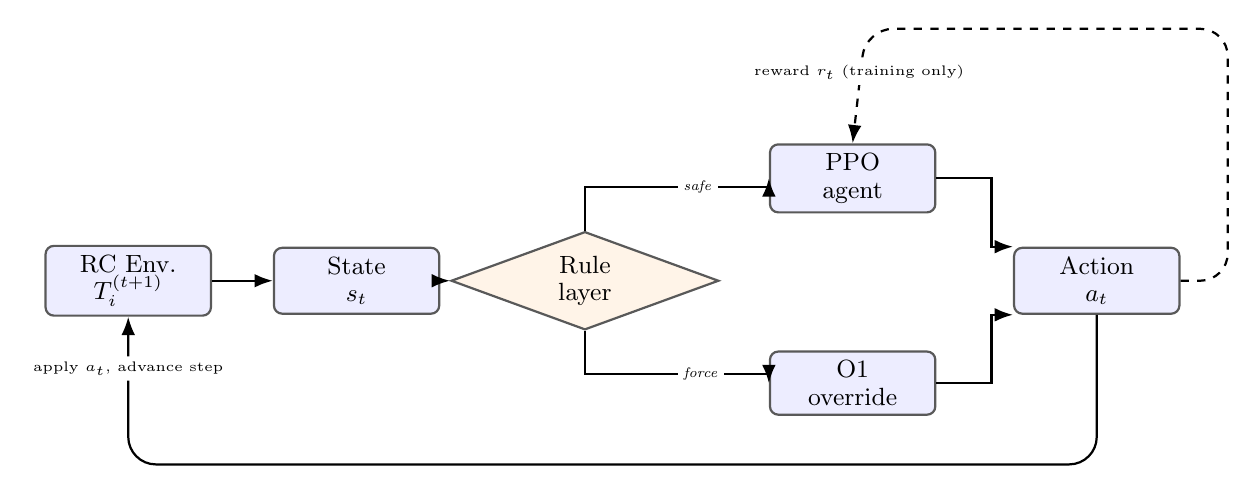
\begin{tikzpicture}[
  box/.style={rectangle,draw=black!65,rounded corners=3pt,thick,
              minimum width=2.1cm,minimum height=0.76cm,
              align=center,fill=blue!7,font=\small},
  dec/.style={diamond,draw=black!65,thick,aspect=2.4,
              fill=orange!9,align=center,font=\small,
              minimum width=3.4cm,minimum height=0.72cm},
  arr/.style={-Latex,thick},
  note/.style={font=\tiny,inner sep=2pt,fill=white,draw=none}]
%%
%% Nodes
\node[box](env)   at ( 0.0,  0  ) {RC Env.\\[-1pt]$T_i^{(t+1)}$};
\node[box](state) at ( 2.9,  0  ) {State\\[-1pt]$s_t$};
\node[dec](rule)  at ( 5.8,  0  ) {Rule\\[-1pt]layer};
\node[box](rl)    at ( 9.2,  1.3) {PPO\\[-1pt]agent};
\node[box](ovr)   at ( 9.2, -1.3) {O1\\[-1pt]override};
\node[box](act)   at (12.3,  0  ) {Action\\[-1pt]$a_t$};
%%
%% Main pipeline: env → state → rule
\draw[arr](env) -- (state);
\draw[arr](state) -- (rule);
%%
%% Branch from rule.north → PPO (safe path, above)
\draw[arr](rule.north) -- ++(0,0.55) -| node[note,right,pos=0.25]{\textit{safe}} (rl.west);
%%
%% Branch from rule.south → override (force path, below)
\draw[arr](rule.south) -- ++(0,-0.55) -| node[note,right,pos=0.25]{\textit{force}} (ovr.west);
%%
%% PPO → action (upper path)
\draw[arr](rl.east) -- ++(0.7,0) |- (act.north west);
%%
%% Override → action (lower path)
\draw[arr](ovr.east) -- ++(0.7,0) |- (act.south west);
%%
%% Smooth feedback loop: action → env (routed below override)
\draw[arr,rounded corners=10pt] (act.south)
  -- ++(0,-1.9)                 % go below the diagram
  -- ++(-12.3,0)                % move left under all boxes
  -- ++(0,0.9)                  % go up toward env
  -- (env.south)
  node[note,below,midway]{apply $a_t$, advance step};
%%
%%
%% Smooth reward loop: action → PPO (dashed)
\draw[arr,dashed,rounded corners=10pt] (act.east)
  -- ++(0.6,0)                % move right of Action
  -- ++(0,3.2)                % go vertically above PPO
  -- ++(-4.6,0)               % move left toward PPO
  -- (rl.north)               % connect from above
  node[note,above,midway]{reward $r_t$ (training only)};
\end{tikzpicture}}% end resizebox
\caption{RBRL architecture. The rule layer routes to the PPO agent when no
comfort boundary is threatened (\emph{safe}) and overrides it with the
O1-enforcing action when one is imminent (\emph{force}); the dashed reward
loop is used in training only.}
\label{fig:framework}
\end{figure*}
 
\subsection{State Space}
\label{subsec:state}
 
The numerical study controls a single zone, and at interval $t$ the agent
observes eight features:
\begin{equation}
\begin{split}
  s_t=\Bigl(&T^{(t)},\;u^{(t-1)},\;\Tout^{(t)},\;\Tout^{(t+4)},\;I^{(t)},\\
  &\sin\tfrac{2\pi h_t}{24},\;\cos\tfrac{2\pi h_t}{24},\;t/N\Bigr)\in\Rset^{8},
\end{split}
  \label{eq:state}
\end{equation}
namely the zone temperature, the previous action, the outdoor temperature now
and one hour ahead, the south-vertical irradiance, the hour of day as a
sine--cosine pair, and the fraction $t/N$ of the episode elapsed, each scaled
to order one (scalings in the repository). The one-hour outdoor value is a
perfect forecast. The effective inter-zone temperature $\Tiz{i}$
(equation~\eqref{eq:tiz}) is not observed, because there is no neighbouring
zone, and neither is $E_{\mathrm{cum}}$: under the in-force two-block tariff
this dwelling never leaves the first block (Remark~\ref{rem:current_tariff}),
so the cost rate does not depend on it. A learned multi-zone or
stepped-tariff policy would need both; none is trained here.

\subsection{Rules and Action Space}
\label{subsec:rules}
 
\begin{definition}[Rule-based overrides]
\label{def:rules}
\begin{align}
  &\textbf{R1}\;(\text{hard, force on:})\;
    T_i^{(t)}\ge\Tmax-\epsilon_{\mathrm{hot}}
    \;\Rightarrow\;u_i^{(t)}\leftarrow1. \label{eq:R1}\\
  &\textbf{R2}\;(\text{hard, force off:})\;
    T_i^{(t)}\le\Tmin+\epsilon_{\mathrm{cold}}
    \;\Rightarrow\;u_i^{(t)}\leftarrow0. \label{eq:R2}
\end{align}
\end{definition}

The guard bands are \emph{asymmetric} and are derived, not assumed. Each
must absorb the temperature excursion of one actuation interval in its own
direction:
\begin{equation}
\begin{aligned}
  \epsilon_{\mathrm{cold}}&\ge\frac{\Qhvac\Delta t}{\Cth},\\
  \epsilon_{\mathrm{hot}}&\ge\frac{\Delta t}{\Cth}\max_t\!\left[\Lambda_i(\Tout^{(t)}{-}\Tmax)+Q_{\mathrm{sol}}^{(i,t)}\right].
\end{aligned}
  \label{eq:guard}
\end{equation}
The two differ because cooling is driven by the plant and warming by the load.
At the parameters of Table~\ref{tab:params} the cooling excursion is
$0.375\,^\circ$C; the peak seasonal load of $690$, $664$ and $513\,$W across the
three cities gives warming excursions of $0.129$, $0.125$ and
$0.096\,^\circ$C. Cooling is about $2.9$ times the fastest warming, so
$\epsilon_{\mathrm{cold}}=0.40$ and $\epsilon_{\mathrm{hot}}=0.20\,^\circ$C are
adopted, so the agent acts on $(22.40,23.80)$ rather than the $(22.5,23.5)$ a
symmetric $0.5\,^\circ$C guard would leave. Even so,
the rule layer can exclude the tuned thermostat's own switch points
($23.71/22.36$, $23.70/22.34$ and $23.64/22.32\,^\circ$C in Riyadh, Jeddah
and Taif, all with an off point below R2): that exclusion is a property of the
method, since any fixed guard band forbids some members of the family it
guards.

The rule layer contains no pre-cooling rule, because
Proposition~\ref{prop:path} and Remark~\ref{rem:energy_identity} rule it out
under every cost model used here. Pre-cooling would pay only under a physical
condition, not a tariff one: shifting cooling from $t_2$ back to
$t_1$ pays only if the price of \emph{delivered} cooling falls by more than the
store leaks over the interval, which at $\tau=\Cth/\Lambda_i=56.1\,$h is
$3.5\%$ over a four-hour shift and $6.8\%$ over eight, averaged over the
shift; the end-point figures $1-e^{-\Delta t/\tau}$ are $6.9\%$ and
$13.3\%$. A cumulative-block tariff
supplies none of that. A temperature-dependent coefficient of performance would
supply $15$--$20\%$ across a typical diurnal swing and is the route by which a
pre-cooling rule could be reinstated (Section~\ref{subsec:limits}). R1 and R2 enforce
O1 by construction, not by training.
The action is $a_t=(u_1^{(t)},\ldots,u_{N_z}^{(t)})\in\{0,1\}^{N_z}$.
A single PPO head is used.
 
\subsection{Reward Function and PPO Architecture}
\label{subsec:reward}
 
The per-step reward is the negative interval cost minus a linear
degree-hour comfort penalty:
\begin{equation}
  r_t=-c^{(t)}-\alpha\Bigl[\max\!\bigl(0,T^{(t+1)}-\Tmax\bigr)
       +\max\!\bigl(0,\Tmin-T^{(t+1)}\bigr)\Bigr]\Delta t,
  \label{eq:reward}
\end{equation}
with $\alpha=50\,\SAR$ per $^\circ$C\,h, and at the last step of an episode the
terminal thermal state is priced exactly as the dynamic programme and the
simulator price it. Under the rule layer the penalty is zero except on
plant-limited cold drift.
The policy and value networks are separate, each with two fully connected
layers (256--128 units, $\tanh$); the policy outputs the logits of a
categorical distribution over $u\in\{0,1\}$. Training uses Stable-Baselines3
v2.9.2 \citep{Raffin2021} with Adam at a constant learning rate of
$3\times10^{-4}$, $\gamma=0.999$, clip coefficient $0.2$, entropy coefficient
$0$, rollouts of $1{,}344$ steps (two episodes) with minibatches of $336$, and
otherwise default settings; no hyperparameter search was made. Training runs
for $2\times10^{5}$ environment steps (about $298$ episodes of $672$ steps, one
$168\,$h window at $\Delta t=15\,$min) with five seeds ($42$--$46$), none
discarded, a fixed budget and no checkpoint selection; each episode draws its
start date from the six tuning windows of Section~\ref{subsec:protocol}. During
training the ceiling is the band edge, $\overline{T}=\Tmax$, so R1 fires at
$23.80\,^\circ$C and R2 at $22.40\,^\circ$C.

No convergence claim is made. With the rules on and a flat price, the
training reward, which has no term in the mean temperature, is nearly
minimised by holding the previous action until a rule fires (within $0.4$,
$1.4$ and $2.3\%$ of the exact $\lambda=0$ dynamic-programming optimum inside
the rules, called E1; Section~\ref{subsec:abl_component}). In Riyadh and Jeddah the seeds learn that
policy: eight of ten runs reproduce the guard hysteresis's pooled saving to
$10^{-5}$, and the other two differ by less than $0.004$ points; in Taif four
of five seeds fall below it. That shortfall is one of generalisation, not of
training length: scored with the training cost at the training rules, three of
those four seeds are within $0.05\%$ of the hold policy on the six tuning weeks
(the fourth $1.4\%$) and $0.5$--$2.5\%$ above it only on the held-out weeks, so
a longer run on the same weeks has almost nothing left to gain.
A second variant, E2, tests whether this is a property of the reward: it adds
the stage term $(\lambda/n_{\mathrm{occ}})\max(T^{(t+1)},\Tmin)$ of the
receding-horizon controller, with $\lambda$ taken from the in-rules $6\,$h
controller, and a perfect outdoor forecast at $+1$, $+2$, $+3$ and $+6\,$h and
irradiance at $+1$ and $+3\,$h to the state; it is trained in Riyadh with three
seeds, an entropy coefficient of $0.01$ and reward normalisation, under the
same rules in training and evaluation, with no Rule~A selection. It stays
close to the rules' hold policy (Section~\ref{subsec:abl_component}).
Algorithm~\ref{alg:rbrl} sets out training and schedule extraction together; the
policy $\pi_\theta$ it returns is the one evaluated in every RBRL row of
Section~\ref{sec:results}.
 
\begin{algorithm}[H]
\caption{RBRL: training, ceiling selection and evaluation}
\label{alg:rbrl}
\begin{algorithmic}[1]
\Require simulator~\eqref{eq:rc_scalar}; tuning windows $\mathcal{W}_{\mathrm{tune}}$
  and held-out windows $\mathcal{W}_{\mathrm{eval}}$ (start dates $d_0$, $N=672$
  steps each); price $p$; $\csw$; budget $B=2\times10^{5}$ steps; guard
  margins $\epsilon_{\mathrm{hot}},\epsilon_{\mathrm{cold}}$; ceiling grid
  $\mathcal{C}=\{23.50,23.51,\dots,24.00\}\,^\circ$C
\Ensure policy $\pi_\theta$, ceiling $\overline{T}^{*}$, held-out costs
  $\{J_w\}_{w\in\mathcal{W}_{\mathrm{eval}}}$
\Statex \textbf{Phase 1: training} ($\overline{T}=\Tmax$)
\State Initialise $\pi_\theta$; $n\leftarrow0$
\While{$n<B$} \Comment{fixed budget; no early stopping}
  \State Draw $d_0\in\mathcal{W}_{\mathrm{tune}}$; $T^{(0)}\leftarrow23\,^\circ$C, $u^{(-1)}\leftarrow0$
  \For{$t=0$ \textbf{to} $N-1$}
    \State observe $s_t$~\eqref{eq:state}; $a_t\sim\pi_\theta(\cdot\,|\,s_t)$
    \State $u^{(t)}\leftarrow\mathcal{R}(a_t,T^{(t)};\overline{T})$ \Comment{R1--R2, eq.~\eqref{eq:guard}}
    \State step~\eqref{eq:rc_scalar}; $r_t$ by~\eqref{eq:reward}; $n\leftarrow n+1$
  \EndFor
  \State add the terminal price of $T^{(N)}$ to $r_{N-1}$
  \State every $1{,}344$ steps: PPO update (clipped surrogate, GAE)
\EndWhile
\Statex \textbf{Phase 2: R1-ceiling selection on the tuning windows (Rule~A)}
\For{$\overline{T}\in\mathcal{C}$}
  \State run $\arg\max_a\pi_\theta$ with $\mathcal{R}(\cdot;\overline{T})$ on every $w\in\mathcal{W}_{\mathrm{tune}}$
\EndFor
\State $\overline{T}^{*}\leftarrow$ admissible $\overline{T}$ (Rule~A) of least
  equalised tuning cost ratio
\Statex \textbf{Phase 3: held-out evaluation (frozen $\pi_\theta$, $\overline{T}^{*}$)}
\For{$w\in\mathcal{W}_{\mathrm{eval}}$}
  \State run $\arg\max_a\pi_\theta$ with $\mathcal{R}(\cdot;\overline{T}^{*})$; record $J_w$ and $\tilde{\bar T}_w$
\EndFor
\State\Return $\pi_\theta$, $\overline{T}^{*}$, $\{J_w\}$ \Comment{compared by Rule~C, Section~\ref{subsec:protocol}}
\end{algorithmic}
\end{algorithm}
 
\subsection{Competing Methods}
\label{subsec:compete}
 
\textbf{THERM (unoptimised baseline)} models the automatic remote-controller thermostat common in Saudi residential buildings \citep{Alotaibi2024}: on when $T_i\ge\Tmax-0.5$, off when $T_i\le\Tmin+0.5$, with no tariff awareness.
On the occupied band adopted here this is a $1\,^\circ$C deadband centred on
$23\,^\circ$C, assumed, not measured, to represent the split units in this
stock (Section~\ref{subsec:abl_component}). Every optimising controller gains
over THERM by using more of the $2\,^\circ$C band under the same comfort
obligation.

\textbf{TUNED (rule-based comparator)} is the same hysteresis family with its two
switch points free. They are searched on a $0.05\,^\circ$C grid and then
refined iteratively on a $0.01\,^\circ$C grid around the best admissible pair;
a row at the $0.1\,^\circ$C resolution of typical hardware is in the
supplement. Without TUNED, any gap attributed to learning or planning may in
fact be obtainable by commissioning the thermostat properly.

\textbf{Guard hysteresis} is the hysteresis at the rule layer's own thresholds,
R1 and R2, with no learned policy: on at $\overline{T}-\epsilon_{\mathrm{hot}}$,
off at $\Tmin+\epsilon_{\mathrm{cold}}$, with the ceiling $\overline{T}$ fitted
like every other parameter. \textbf{D1} is a one-step model shield on a latch
that holds the previous action and has no R1/R2 guard bands: it forces the
unit on when the exact one-step prediction with the unit off would end above
$\overline{T}-\sigma$, and off when the prediction with it on would end below
$\Tmin+\sigma$, with its own ceiling $\overline{T}\le\Tmax$ fitted for each
margin $\sigma\in\{0,0.05,0.10\}\,$K; on the trained PPO policies it replaces
the rule layer. It needs the plant model and the current outdoor temperature and
irradiance, where TUNED needs only the zone temperature. D1 separates what an exact one-step model buys from what a longer
horizon buys.

\textbf{MPC (causal receding-horizon comparator, also ``the planner'').} At every step the
controller solves, by dynamic programming over a temperature grid with the
first step taken from the exact state, the horizon problem with stage cost
$c^{(t)}+(\lambda/n_{\mathrm{occ}})\max(T^{(t+1)},\Tmin)$ over occupied steps,
applies the first action and re-solves. Cooling steps that would end below
$\Tmin$ are infeasible, as for every optimiser here. The multiplier $\lambda$
is the comfort device: one value per city, horizon and forecast mode, fitted on
the tuning windows by Rule~A of Section~\ref{subsec:protocol} and then frozen.
If no multiplier is admissible even at the $0.10\,$K fallback, the planner's
occupied ceiling is lowered by a back-off $b$ fitted by the same rule (cells
marked $\dagger$); the order is $\lambda$ at $0.03\,$K, then $\lambda$ at
$0.10\,$K, then $b$. For the $6$ and $24\,$h perfect-forecast controllers the
fitted values lie within $2.5\%$ of
$\lambda^\ast=\Lambda_i\,(168\,\mathrm{h})\,p/\mathrm{COP}$, the marginal
envelope cost of $1\,$K over a window, at which the Lagrangian is indifferent
to the temperature level; the controller therefore minimises on-commands and
its comfort level is set by the Rule~A selection of $\lambda$. Close to
$\lambda^\ast$ the result is sensitive to $\lambda$: in Riyadh, neighbouring
admissible multipliers give $24\,$h savings that differ by $1.4$--$1.8$ points
at both grid resolutions, so the fitted $\lambda/\lambda^\ast$ is reported in
Section~\ref{subsec:ladder}. The horizon problem is closed by a rollout terminal cost: the
cost, including the on-command charge and the $\lambda$ term, of running TUNED
for $24\,$h from the terminal state on a persistence forecast, plus the price
of the stored heat. This is a truncated rollout of a base
policy \citep{Bertsekas2020}; the classical guarantee of closed-loop cost no
greater than the base policy's does not carry over, because the tail is
truncated, uses persistence weather and is evaluated on a grid, so any
improvement over TUNED is an empirical finding. Horizons of $0.25$, $1$, $2$,
$6$, $24$ and $48\,$h are run with two forecast modes: \emph{perfect}, the
true in-horizon weather, and \emph{persistence}, in which the forecast for
step $j$ is the observation one day earlier, with the current outdoor
temperature measured. In both modes the controller plans on the plant's own
model with the exact state. The \emph{in-rules} variant restricts every action to the training rule
set, R1/R2 at $23.80/22.40\,^\circ$C; its terminal rollout still uses TUNED,
whose off point lies below R2. The value grid has $1{,}601$ nodes;
at the fitted $\lambda$, refining it to $3{,}201$ nodes changes the $24\,$h
saving by $0.10$, $0.45$ and $0.29$ points in Riyadh, Jeddah and Taif; the
grid uncertainty is therefore taken as at most $0.5$ points, below the
$3$-point resolution rule.

\textbf{CLV (clairvoyant reference)} is a dynamic programme over the exact
dynamics~\eqref{eq:rc_disc} that sees the whole window's weather. Its
multiplier is set per held-out window, by bisection (with an occupied-ceiling
cap as a second knob where needed), aiming at a clipped mean
within $0.002\,$K of THERM's. At the critical multiplier the optimal
schedule's mean jumps by $0.1$--$0.3\,$K, so the target is met in only $2$ of
$7$ windows in Riyadh, $1$ of $7$ in Jeddah and none in Taif;
elsewhere the closest schedule no warmer than THERM is kept, and its residual
is recorded (per window in the supplement).

\emph{End-of-window convention.} The simulator, and so every causal arm,
prices the terminal thermal state at the electricity needed to return it to
the initial temperature $T_0$ at rated COP. A programme that knows where the
window ends could exploit that price, because it omits the on-command the
return would need. The oracles (CLV, the bound and $B_a$) therefore use
$V_N=\bigl[p\,\Cth/(3.6\times10^{6}\,\mathrm{COP})+\csw/(1\,\mathrm{K})\bigr](T_N-T_0)$:
heat left above $T_0$ is charged its re-cooling energy plus the fraction
$(T_N-T_0)/1\,$K of one on-command, that is, one on-command per kelvin, which
is a convention. The savings of the causal arms in Table~\ref{tab:main} use the
simulator terminal, the bracket and $B_a$ use $V_N$, and $B^\ast$ is also
reported under the simulator terminal for Riyadh and Jeddah. E1 keeps the
simulator terminal, which is PPO's own objective. CLV and the bound of Section~\ref{subsec:bound}
bracket what a schedule no warmer than the baseline could save; the gap between
TUNED and that bracket is the headroom any controller could in principle
occupy.

Genetic-algorithm and simulated-annealing schedulers \citep{ElMakroum2023,Bandarra2025}
are not run. Both are day-ahead offline solvers, and the bound
of~\eqref{eq:dual_bound} applies to them as to every other schedule at the
baseline's mean, so it answers the question they would be introduced to
answer. No third-party learned comparator (SAC, DQN) is run inside the rule
layer either. A relaxed bound restricted to the training rule set
($14.9$, $15.6$ and $16.2\%$ in Riyadh, Jeddah and Taif) caps what any such
learner could attain, but whether another learner would come closer to it than
PPO is untested, as is any learner acting outside R1--R2.
 
The framework is applied to the three climates characterised next.
 
%% ============================================================
\section{Case Studies: Riyadh, Jeddah and Taif}
\label{sec:casestudy}

Three sites are used, chosen to span the conditions under which a Saudi dwelling
is cooled, not to represent the Kingdom: hot-arid inland (Riyadh),
hot-humid coastal (Jeddah) and mild highland (Taif).
 
\subsection{Climate Profiles}
\label{subsec:climate}
 
Riyadh (BWh, $24.7^\circ$N, $635\,$m) is an inland desert city with summer highs
reaching $46.6\,^\circ$C and a cooling-season diurnal swing of $12.7\,$K, the
largest of the three sites (CDD$_{18}=3{,}693$; cf. \citep{Haddad2024}).
Jeddah (BSh, $21.7^\circ$N, $15\,$m) is a Red Sea coastal city, classified
hot-humid \citep{Rodrigues2025}; in the record used here its annual mean
relative humidity is $58.5\%$ with $17.5\%$ of hours above $70\%$, and it has a
compressed diurnal swing of $8.4\,$K and little overnight relief
(CDD$_{18}=4{,}260$; the ordering of the two totals depends on the
typical-year record, and what distinguishes the sites here is the diurnal
swing).
Taif (BSh, $21.5^\circ$N, $1{,}478\,$m) is a highland site whose altitude lowers
both the peak and the mean: over the cooling season its mean outdoor temperature
is $28.6\,^\circ$C against Riyadh's $35.0$ and Jeddah's $32.7$; its peak
$39.4\,^\circ$C against $46.6$ and $44.0$; and its CDD$_{18}=2{,}277$ against
$3{,}693$ and $4{,}260$. Its diurnal swing, $11.7\,$K, is
close to Riyadh's. The load is therefore the smallest of the three while the
headroom is not, which is why Taif leaves the least to schedule in absolute
terms; the lower air density at that altitude is
also why the infiltration conductance is evaluated per city
(Section~\ref{subsec:sbc}); monthly and diurnal profiles are in the repository.
All three simulations use
TMYx typical-year records from
\texttt{climate.onebuilding.org}, WMO~404380 (Riyadh, period of record
2009--2022, $12$ years of data), 410240 (Jeddah, 2009--2023, $15$ years) and
410360 (Taif, 2009--2023, $15$ years); hourly dry-bulb temperature
and the direct-normal and diffuse-horizontal irradiances are read from
fields~7, 15 and~16, and the glazing gain is the plane-of-array irradiance on a
south-facing vertical surface under an isotropic sky with ground albedo
$0.30$.
 
 
\subsection{Building Code, Tariff, Humidity, and Comfort Standard}
\label{subsec:sbc}
 
SBC~2018 mandates opaque-wall U-value $\le0.45\,\text{W\,m}^{-2}\text{K}^{-1}$ and window SHGC $\le0.25$ in both Climate Zone~A (Jeddah) and Zone~B (Riyadh) \citep{Alayed2021}. Table~\ref{tab:params} meets both at assembly level: $U_{\mathrm{wall}}=0.45$ and $\mathrm{SHGC}=0.25$ exactly, with $U_{\mathrm{win}}=2.8\,\text{W\,m}^{-2}\text{K}^{-1}$ consistent with double glazing.
The multi-tier step-wise tariff follows equation~\eqref{eq:stepwise}; for Models~L and~E, $c_r^{\mathrm{L}}=0.12\,\SAR/\kWh$ is adopted as an illustrative flat rate, below the post-2018 first-block price of $0.18\,\SAR/\kWh$. It is \emph{not} the consumption-weighted average of~\eqref{eq:stepwise} over this account, which at ${\approx}884\,\kWh$ is the first-block rate of $0.05\,\SAR/\kWh$ exactly.
The occupied comfort band $[22,24]\,^\circ$C is consistent with the \emph{thermal} criterion of ASHRAE~55-2023 \citep{ASHRAE55_2023} for mechanically conditioned residential spaces (the standard's humidity criterion is not evaluated here; Section~\ref{subsec:disc_limits}). \citet{Bienvenido2024} validate this use, and its upper limit reflects Saudi practice: \citet{Krarti2020occ} recommends $23$--$25\,^\circ$C for Kingdom dwellings and observes setpoints as low as $18\,^\circ$C in the stock.
\citet{Lamsal2023} review adaptive thermal comfort models and find wider deadbands appropriate for energy-efficient design in hot climates; the narrower band adopted here raises the reported saving through the baseline's cycling (Section~\ref{subsec:disc_band}) and was not swept.
A fixed band is adopted because Saudi residential buildings are predominantly mechanically cooled; ASHRAE~55 Section~5.3 restricts adaptive comfort to naturally ventilated spaces.
The saving does not transfer across band widths, because the actuation condition~\eqref{eq:deadband_condition} and the baseline's cycling rate both depend on the width.
 
 
%% ============================================================
\section{Simulation Setup}
\label{sec:sim}
 
The controllers of Section~\ref{sec:method} are evaluated on the sites of
Section~\ref{sec:casestudy} under one protocol, set out here.
All simulations run in Python~3.13.18 with NumPy~2.5.3, integrating
equation~\eqref{eq:rc_disc} exactly at $\Delta t=15\,$min, the interval that
satisfies~\eqref{eq:deadband_condition} with a factor of $2.7$
(Remark~\ref{rem:rc}). Solar gain is
$Q_{\mathrm{sol}}^{(i,t)}=\text{SHGC}\times A_{gl}\times I^{(t)}$, with
$I^{(t)}$ the plane-of-array irradiance of Section~\ref{subsec:climate}; hourly
weather values are held constant over the intervals of each hour, without
interpolation. The RC model has no occupancy or internal gains.

\paragraph{Background load and tariff.}
The tariff is levied on the whole account, so the cumulative energy
$E_{\mathrm{cum}}$ starts from a non-HVAC load of
$E_{\mathrm{base}}\approx800\,\kWh$/month \citep{AlHomoud2021}. The single
zone adds about $84\,\kWh$ a month, so the account reaches ${\approx}884\,\kWh$
and crosses no boundary of any schedule; sixteen such zones would approach the
first boundary of the historical four-tier schedule, which is why Model~S is
kept as a stress test (Remark~\ref{rem:current_tariff}).

\paragraph{Evaluation protocol.}
\label{subsec:protocol}
Evaluation is confined to the cooling season, 1~May to 31~October, because the
plant is cooling-only. Thirteen windows of $168\,$h start every $14$ days,
at zero-based day indices $121$ to $289$ (1~January is day~$0$), none
overlapping, and are assigned alternately within one TMYx year. The seven
\emph{held-out} windows start on 2~May, 30~May, 27~June, 25~July, 22~August,
19~September and 17~October; the six \emph{tuning} windows start on 16~May,
13~June, 11~July, 8~August, 5~September and 3~October. There is no separate validation set: every
parameter, including PPO's ceiling, is selected on the tuning windows alone,
PPO trains for a fixed budget with no early stopping or checkpoint selection,
and the held-out windows are touched only once, for evaluation. The seven
held-out windows span the cooling season, so the seasonal variation is carried
by the per-window tests rather than by a separate seasonal evaluation; the
inter-annual spread is measured on actual years (Section~\ref{subsec:robustness}).
One protocol, implemented in one code module, applies to every arm and oracle.

\emph{Comfort.} On every occupied step the post-step temperature must not
exceed $\Tmax$; the occupied over-temperature in degree-hours is recorded for
every arm. On the cold side, \emph{cooling may never end a step below $\Tmin$;
free-float is unrestricted}: $u^{(t)}=1$ implies $T^{(t+1)}\ge\Tmin$ at every
step, and $u^{(t)}=0$ has no lower limit. Sub-band states can therefore arise
only by free drift when the off-state equilibrium lies below the band. In the
optimisers this is a hard constraint on cooling transitions. The rule-layer
arms and D1 are designed to meet it from the nominal plant parameters, and
TUNED meets it on the tuning windows by Rule~A and threshold placement, not by
guarantee; for all of them it is measured as commanded under-temperature, the
degree-hours below $\Tmin$ at the end of cooling steps, reported beside the
free-float under-temperature of idle occupied steps.

\emph{Rule~A (selection on the tuning windows).} Each causal arm has one
parameter set per city: TUNED's two switch points, the guard's and RBRL's
ceiling, D1's margin $\sigma$, and the receding-horizon controller's $\lambda$
for each horizon and forecast mode. A candidate is admissible if, on every
tuning window, it has zero over-temperature and zero commanded
under-temperature, and if its clipped mean occupied temperature pooled over the
tuning windows lies within $0.03\,$K of THERM's. Among admissible candidates
the one with the least equalised tuning cost ratio
$\sum_wJ_w/\sum_wJ_{\mathrm{THERM}(\delta_w),w}$ (Rule~C applied to the tuning
windows) is selected and frozen. If no candidate meets the $0.03\,$K
condition, it is relaxed to $0.10\,$K, for every arm alike; each table states
which applies (\texttt{fit\_status}), and an arm with no admissible parameter
is reported as such and not tabulated. A sensitivity refit under a per-window
$0.03\,$K criterion is in the supplement.

\emph{Rule~B (clipped mean).} Occupied means are computed on
$\tilde T=\max(T,\Tmin)$ for every arm and for THERM, so a free-float cold
excursion buys no credit against warmth elsewhere.

\emph{Rule~C (equalisation per held-out window).} On each held-out window $w$
the frozen arm is compared with THERM shifted by $\delta_w$ (on at
$23.5+\delta_w$, off at $22.5+\delta_w$), with $\delta_w$ scanned over
$[-0.4,0.4]\,$K in $0.002\,$K steps. THERM's clipped mean is not monotone in
$\delta$, so the arm's mean can be reached at several shifts; the comparator
cost is the \emph{minimum} over all crossings of the piecewise-linear scan,
interpolated linearly within each bracketing segment, which credits the
baseline with its cheapest setting of equal comfort and can only understate a
saving. Scored this way, the unshifted thermostat itself saves
$-0.8$, $-0.1$ and $0.0\%$ in Riyadh, Jeddah and Taif, which is the size of the rule's
conservatism; the range between the cheapest and the dearest crossing is in
the supplement. The only saving printed is the pooled
\begin{equation}
  s=1-\frac{\sum_{w}J_{\mathrm{arm},w}}{\sum_{w}J_{\mathrm{THERM}(\delta_w),w}},
  \label{eq:saving}
\end{equation}
over the seven held-out windows; the raw saving against unshifted THERM, the
pooled and largest per-window mean differences, the comfort metrics and the
pooled end temperature are printed beside it. Per-window savings enter only
the tests. No held-out window contributes to any arm's parameters. CLV is
matched per held-out window (Section~\ref{subsec:compete}), and the bound
needs no selection (Section~\ref{subsec:bound}).

\emph{Statistics.} The unit is the per-window difference in equalised saving
between two arms on the same seven windows. Each contrast is tested with the
exact two-sided Wilcoxon signed-rank and sign tests and summarised by the
Hodges--Lehmann estimate with an exact $95.3\%$ interval (the third smallest
and largest of the $28$ Walsh averages); the estimate and interval lead, the
$p$-value is secondary. The primary families, each one contrast in three
cities with Holm's correction within the family, are TUNED against THERM, MPC
($24\,$h, perfect) against TUNED, MPC ($24\,$h, persistence) against TUNED, and
the guard against TUNED; E2 is not tested against the guard, because its
comfort is not matched to the other arms. With $n=7$ and three cities, $0.047$
is the smallest Holm-adjusted $p$ attainable, reached by a city only when all
seven of its windows agree in sign; one discordant window removes
significance, and such results are reported as counts. The horizon, capacity,
switching-charge, deadband and tariff sweeps are descriptive. Pooled
differences of less than $3$ points between arms are treated as not resolved,
whatever a test says, because the occupied-mean staircase and the tuning noise
are of that order; the threshold does not absorb comfort offsets between arms
(Section~\ref{subsec:limits}). The held-out weeks come from
one TMYx year, so the tests describe those weeks. Estimates, intervals,
$p$-values and comfort offsets for every family are in Supplementary Table~S8.

\emph{Switching charge.} For a split unit of ${\sim}2{,}500\,\SAR$ installed
cost, a start life of order $10^{5}$ gives $0.025\,\SAR$ per start, and a
$15$-year life at about $1{,}460$ on-commands a year (four a day all year)
gives about $0.114\,\SAR$; counting only the $184$-day cooling season at
THERM's $4.10$ a day would give about $0.22\,\SAR$. The range
$0.025$--$0.114\,\SAR$ per on-command is therefore a convention, not a measured
wear cost; none was found for Saudi split units \citep{Pang2011}. The tables use
$\csw=0.15\,\SAR$ as the computational reference, because the PPO policies were
trained at it; it lies above the derived range and overstates the saving
against it, since the saving rises with $\csw$. Results at $0.025$ and $0.114\,\SAR$ are
reported beside it (Section~\ref{subsec:abl_component}). The cost figures are
therefore a pricing of the on-command reduction, which is the quantity
actually measured.
 
%% ============================================================
\section{Results}
\label{sec:results}

Results are reported on the seven held-out windows at the tariff in force,
$\csw=0.15\,\SAR$, $\Delta t=15\,$min and $\Cth=4{,}800\,\text{kJ/K}$, with
the receding-horizon controller on a $1{,}601$-node grid. Every fitted
single-zone arm records zero occupied over-temperature on the held-out windows;
the two fixed
setback arms do not (Section~\ref{subsec:consumption}). Commanded
under-temperature (Supplementary Table~S4) is zero for every optimiser,
rule-layer and D1 arm except the Riyadh $6\,$h persistence controller, whose
plan meets the cold rule on the forecast but not on the realised weather
($0.0006\,^\circ$C$\cdot$h over the seven windows). The multi-zone controller,
which plans each room against its neighbours' plans of the previous step, records
$0.0001\,^\circ$C$\cdot$h of occupied over-temperature in the $1\times4$ row at
$\lij=35\,$W/K and at most $0.00003\,^\circ$C$\cdot$h of commanded
under-temperature in the $2\times2$ grid. The threshold arms meet
it only on the tuning windows: on the held-out windows TUNED records $0.0007$
and $0.0066\,^\circ$C$\cdot$h in Jeddah and Taif, and TUNED-SB
$0.0102\,^\circ$C$\cdot$h in Riyadh, the largest in the headline
configuration ($0.024\,^\circ$C$\cdot$h at most in any sensitivity run). The largest free-float value, $0.96\,^\circ$C$\cdot$h, belongs to the Taif $24\,$h
persistence controller, and in Taif TUNED and the guard also free-float below
the band ($0.29$ and $0.34\,^\circ$C$\cdot$h). Section~\ref{subsec:bound} first fixes what clairvoyance is
worth; Sections~\ref{subsec:consumption}--\ref{subsec:multizone} then read the
controllers against it.
 
\subsection{What Clairvoyance Is Worth: a Bound and an Attained Schedule}
\label{subsec:bound}

The bound keeps comfort pointwise and applies the comfort match only in the
mean, so it covers every schedule no warmer than the baseline:
\begin{equation}
\begin{split}
  \min_{u}\;&J(u)\quad\text{s.t.}\quad
    T^{(t+1)}\le T^{\mathrm{hi}}_t\ \ \forall t,\\
  &u_t=1\;\Rightarrow\;T^{(t+1)}\ge\Tmin\ \ \forall t,\\
  &\tfrac{1}{|\mathcal{O}|}\textstyle\sum_{t\in\mathcal{O}}\tilde T^{(t+1)}
    \;\le\;T^{\star},\qquad \tilde T=\max(T,\Tmin),
\end{split}
\label{eq:meanconstrained}
\end{equation}
with $\mathcal{O}$ the occupied steps, $T^{\mathrm{hi}}_t=\Tmax$ while occupied
and the empty-house limit otherwise, and $T^{\star}$ the baseline's clipped
mean. A cooling step may never end below the band; a free-floating step may,
because a cooling-only plant cannot prevent it, and the clipped mean gives such
an excursion no credit. The mean constraint is an inequality because only
warmth can buy a saving, and because with binary actions on a $15\,$min grid
the attainable means form a finite set. Relaxing it alone gives
$L(u,\lambda)=J(u)+\lambda\bigl(|\mathcal{O}|^{-1}\sum_{t\in\mathcal{O}}\tilde T^{(t+1)}-T^{\star}\bigr)$,
the same dynamic programme with one additive stage cost, and for any
$\lambda\ge0$ and any $u$ feasible for~\eqref{eq:meanconstrained}
\begin{equation}
  J(u)\;\ge\;L(u,\lambda)\;\ge\;\min_{u'}L(u',\lambda)\;=\;L^{\star}(\lambda).
  \label{eq:dual_bound}
\end{equation}
The attained mean is a step function of $\lambda$, so the dual gap need not
close and no exactly mean-matched schedule need exist in the Lagrangian family.

\emph{A provable bound on a grid.} $L^{\star}(\lambda)$ is computed by dynamic
programming on a uniform temperature grid of spacing $h$, and an ordinary
discretised programme can return a minimum that is too \emph{expensive}, the
unsafe direction for a bound. The reported bound therefore uses an
optimistic-neighbour relaxation. For each node $y$, previous action and action
$u$, the exact successor $f_u(y)$ is computed; energy and on-command costs are
charged exactly; the mean term is charged at $\max(f_u(y)-h,\Tmin)$;
feasibility is tested against limits widened by $h$; the continuation is the
smaller of the values at the two nodes bracketing $f_u(y)$; the terminal value
is evaluated at $y-h$; and the initial value is the smaller of the values at
the two nodes bracketing $T^{(0)}$. The grid covers the band plus $0.1\,$K and
extends below it to the window's lowest free-float equilibrium, so no
trajectory admitted by~\eqref{eq:meanconstrained} leaves it.

\emph{Proof.} Take any feasible $u$ with true trajectory $x_t$. Let $y_0$ be
the node bracketing $x_0$ nearest to it, and $y_{t+1}$ the node bracketing
$f_{u_t}(y_t)$ nearest to $x_{t+1}$. The plant map
$f(x)=T_\infty+(x-T_\infty)a$, $a=e^{-\Delta t\Lambda/\Cth}\in(0,1)$, gives
$|f(y_t)-x_{t+1}|=a|y_t-x_t|$, so $|y_t-x_t|\le h$ implies
$|y_{t+1}-x_{t+1}|\le h$, and by induction this holds for every $t$. Along this
path each relaxed stage cost is at most the true one: the mean term because
$f(y_t)-h\le f(x_t)$ and $\lambda\ge0$; the terminal value because it increases
with $T$ and $y_N-h\le x_N$. Every true-feasible step is relaxed-feasible,
because $|f(y_t)-f(x_t)|\le h$ (and, for the rule-constrained variant, whose
masks test the current state, because $|y_t-x_t|\le h$). Because the relaxed
continuation takes the smaller value of the bracketing pair, the relaxed value
at $y_0$ is no larger than the relaxed cost along this path. Hence
$L^{\star}_h(\lambda)\le J(u)+\lambda\bigl(\overline{\tilde T}(u)-T^{\star}\bigr)\le J(u)$
for every $\lambda\ge0$ and every $u$ feasible
for~\eqref{eq:meanconstrained}, pooled over the held-out windows.
$L^{\star}_h$ is concave in $\lambda$, so $\lambda$ is maximised on an
eighteen-point grid with ternary-search refinement; an under-maximised
$\lambda$ weakens the bound without invalidating it. \hfill$\square$

The relaxation has a price. The bracketing minimum may round the successor
down by up to $h$ at every step, and the roundings accumulate over the plant's
memory, $1/(1-a)\approx225$ steps, so the slack is of order $h/(1-a)$ in
temperature and shrinks roughly in proportion to $h$: under $V_N$ the relaxed
saving bound is $21.3$, $20.6$, $20.2$ and $20.0\%$ in Riyadh at $1{,}601$,
$3{,}201$, $6{,}401$ and $12{,}801$ nodes ($21.2$, $20.5$, $20.1$ and $19.8\%$ in
Jeddah), against $19.5\%$ and $19.1$--$19.4\%$ from the ordinary programme,
which is not a bound; at $12{,}801$ nodes the slack is $0.47$ and $0.42$ points.
In Taif the relaxed bound is $23.8$, $22.2$, $21.4$ and $20.9\%$ against
$19.9$--$20.2\%$, a slack of $0.75$ points at $12{,}801$ nodes. Every
grid gives a valid bound, so the smallest is reported, rounded up to $0.1$.
The bound is a minimum over every action sequence in the window under the same
cost, so it holds for any controller whatever information it uses; the
receding-horizon controller's forecast beyond the window end cannot take it
above the bound, because post-window weather enters the cost only through the
terminal price of the stored heat.

\emph{What is reported.} The headline bound is
$B^{\ast}=1-L^{\star}(T^{\star})/\sum_wJ_{\mathrm{THERM}(0),w}$ at THERM's
pooled mean. Each arm $a$ is warmer or cooler than THERM by its own
$\Delta\tilde T$, so its bound is evaluated at its own mean,
$B_a=1-L^{\star}(\overline{\tilde T}_a)/\sum_wJ_{\mathrm{THERM}(\delta^a_w),w}$,
and $s_a\le B_a$ then holds exactly once each arm is rescored under $V_N$;
$B_a$ for the principal arms is in Supplementary Table~S5 (all $89$ rows in the
results files). The lower end of the bracket is the
\emph{best attained schedule no warmer than THERM}, scored as
$1-\sum_wJ_{\mathrm{CLV},w}/\sum_wJ_{\mathrm{THERM}(0),w}$, with the same
denominator and the same mean constraint as $B^{\ast}$; the upper end is the
provable bound under the model; the gap between them is the sum of the
duality gap, the relaxation slack and the replay's own sub-optimality. CLV's
equalised saving under Rule~C is printed only beside $B_{\mathrm{CLV}}$, the
bound at CLV's own mean, never against $B^{\ast}$.

Here the bracket is $[18.0,\,20.0]\%$ in Riyadh, $[18.4,\,19.9]\%$ in
Jeddah and $[16.7,\,21.0]\%$ in Taif, $2.0$, $1.5$ and $4.3$ points wide.
Taif's relaxation slack ($0.75$ points) explains little of its width; the rest
is duality gap and replay sub-optimality, and CLV meets the comfort target in
none of Taif's windows. In an earlier run of the bound under the simulator's
energy-only terminal $B^\ast$ was $20.0$ and $20.1\%$ in Riyadh and Jeddah
(not repeated for Taif). CLV's equalised saving is $18.3\%$ against
$B_{\mathrm{CLV}}=19.6\%$ in Riyadh, $18.5\%$ against $19.4\%$ in Jeddah and
$16.5\%$ against $20.2\%$ in Taif; end-of-window temperatures are in
Supplementary Table~S5. Every arm satisfies $s_a\le B_a$ and
every shifted per-window certificate is non-negative under $V_N$, in all
$89$ arm and seed rows checked (every causal arm, E2, the D1 shield, the
receding-horizon controller in both rule sets, and the setback arms against
the setback bound; the rule-layer arms also against the ruled bound). It is a bracket
at the instance evaluated (the tariff in force, $\csw=0.15\,\SAR$,
$\deadband=1\,^\circ$C, $\Delta t=15\,$min), not at other deadbands or tariffs.

\subsection{Cost, Energy and On-Commands}
\label{subsec:consumption}

Table~\ref{tab:main} gives every arm under the protocol of
Section~\ref{subsec:protocol}, and Table~\ref{tab:layers} reads the principal
arms in three layers. Each saving is the pooled equalised saving against THERM
shifted to the arm's own clipped mean, which removes the first-order energy
effect of the mean temperature; a residual dependence remains (comfort-offset
caveat, Section~\ref{subsec:limits}). Every parameter was fitted on the tuning
windows, so every figure is out-of-sample.

\begin{table*}[t]
\centering
\caption{Held-out results at the tariff in force, occupied band
$[22,24]\,^\circ$C, $\Delta t=15\,$min, $\csw=0.15\,\SAR$, single zone with
one exposed face. $s$: pooled equalised saving~\eqref{eq:saving} (\%);
$\Delta\tilde T$: pooled clipped-mean difference from THERM (K); on: change
in on-commands against the equalised baseline (\%). Fit status:
$^{a}$pooled $0.03\,$K; $^{b}$pooled fallback $0.10\,$K; $^{o}$oracle. Rows
whose $\Delta\tilde T$ differs by more than about $0.02\,$K carry the
comfort-offset caveat (about $1.3$ points per $0.01\,$K,
Section~\ref{subsec:limits}). MPC rows: $1{,}601$ grid nodes, perfect (p) or
persistence (s) forecast; $^{\dagger}$comfort matched by occupied-ceiling
back-off $b$, because the $\lambda$ device alone cannot reach the matched
comfort level. ``training rules'': R1/R2 at $23.80/22.40\,^\circ$C; ``guard
rules'': each city's fitted guard thresholds. D1 rows at $\sigma=0$. CLV:
\emph{raw} saving against unshifted THERM, the best attained schedule no
warmer than THERM; its Rule~C saving is paired with $B_{\mathrm{CLV}}$ in the
text. Causal arms use the simulator's energy-only terminal; the CLV and bound
rows use $V_N$ (Section~\ref{subsec:compete}); $B^\ast$ is given under both.}
\label{tab:main}
\setlength{\tabcolsep}{1.5pt}
\footnotesize
\begin{tabular*}{\textwidth}{@{\extracolsep{\fill}}lrrrrrrrrr@{}}
\toprule
 & \multicolumn{3}{c}{Riyadh} & \multicolumn{3}{c}{Jeddah} & \multicolumn{3}{c}{Taif} \\
\cmidrule(lr){2-4}\cmidrule(lr){5-7}\cmidrule(lr){8-10}
Arm & $s$ & $\Delta\tilde T$ & on & $s$ & $\Delta\tilde T$ & on & $s$ & $\Delta\tilde T$ & on \\
\midrule
THERM ($J$, on/day) & \multicolumn{3}{c}{$1.118$, $4.10$} & \multicolumn{3}{c}{$0.993$, $3.73$} & \multicolumn{3}{c}{$0.614$, $2.33$} \\
TUNED & $12.5^{a}$ & $+0.011$ & $-22.8$ & $13.6^{a}$ & $+0.029$ & $-24.2$ & $12.4^{a}$ & $+0.005$ & $-21.7$ \\
Guard hysteresis & $5.7^{a}$ & $+0.036$ & $-10.5$ & $7.6^{a}$ & $+0.035$ & $-13.6$ & $11.0^{a}$ & $+0.056$ & $-19.3$ \\
RBRL, 5 seeds & $5.7^{a}$ & $+0.036$ & $-10.5$ & $7.6^{a}$ & $+0.035$ & $-13.6$ & $8.6$--$11.0^{a}$ & --- & --- \\
D1 shield on latch & $14.0^{a}$ & $-0.009$ & $-25.4$ & $13.5^{a}$ & $+0.021$ & $-24.0$ & $12.4^{a}$ & $+0.005$ & $-21.7$ \\
D1 on PPO, 5 seeds & $12.8$--$14.1^{a}$ & --- & --- & $11.2$--$13.5^{a}$ & --- & --- & $8.0$--$12.0^{a}$ & --- & --- \\
MPC $0.25\,$h, p & $-3.9^{a}$ & $+0.058$ & $+7.1$ & $1.6^{a\dagger}$ & $+0.023$ & $-2.9$ & $1.0^{a}$ & $+0.034$ & $-1.8$ \\
MPC $1\,$h, p & $10.1^{a\dagger}$ & $+0.024$ & $-18.4$ & $10.1^{a\dagger}$ & $+0.001$ & $-17.9$ & $6.8^{a\dagger}$ & $+0.009$ & $-11.9$ \\
MPC $2\,$h, p & $7.0^{b}$ & $-0.099$ & $-12.7$ & $10.2^{a}$ & $-0.062$ & $-18.2$ & $9.2^{a\dagger}$ & $-0.003$ & $-16.2$ \\
MPC $6\,$h, p & $15.1^{a}$ & $-0.021$ & $-27.4$ & $16.3^{a}$ & $+0.022$ & $-28.9$ & $15.9^{a}$ & $-0.005$ & $-28.0$ \\
MPC $6\,$h, s & $14.4^{a}$ & $-0.004$ & $-26.3$ & \multicolumn{3}{c}{\footnotesize no admissible parameter} & $14.0^{a}$ & $+0.003$ & $-24.6$ \\
MPC $24\,$h, p & $18.3^{a}$ & $+0.014$ & $-33.3$ & $18.1^{a}$ & $-0.011$ & $-32.0$ & $16.9^{a}$ & $-0.011$ & $-29.8$ \\
MPC $24\,$h, s & $12.7^{b}$ & $-0.076$ & $-23.2$ & $14.6^{a}$ & $-0.037$ & $-25.9$ & $10.8^{b}$ & $-0.086$ & $-18.8$ \\
MPC $48\,$h, p & $17.6^{a}$ & $-0.018$ & $-32.0$ & $17.5^{a}$ & $-0.012$ & $-31.1$ & $18.9^{b}$ & $+0.089$ & $-33.4$ \\
MPC $1\,$h, training rules & $9.7^{b}$ & $+0.115$ & $-17.7$ & $-3.6^{a}$ & $-0.053$ & $+6.5$ & $-1.8^{b}$ & $-0.023$ & $+3.1$ \\
MPC $6\,$h, training rules & $10.7^{a}$ & $-0.028$ & $-19.4$ & $10.9^{a}$ & $-0.006$ & $-19.3$ & $11.1^{b}$ & $-0.016$ & $-19.4$ \\
MPC $24\,$h, training rules & $11.6^{b}$ & $-0.061$ & $-21.1$ & $14.1^{a}$ & $-0.003$ & $-24.9$ & $10.0^{b}$ & $-0.064$ & $-17.6$ \\
MPC $1\,$h, guard rules & $2.5^{a}$ & $+0.038$ & $-4.5$ & $1.5^{b}$ & $+0.051$ & $-2.8$ & $8.0^{b}$ & $+0.064$ & $-14.2$ \\
MPC $6\,$h, guard rules & $6.4^{a}$ & $+0.025$ & $-11.7$ & $7.6^{a}$ & $+0.024$ & $-13.5$ & $9.5^{b}$ & $+0.076$ & $-16.7$ \\
MPC $24\,$h, guard rules & $6.7^{a}$ & $+0.028$ & $-12.3$ & $4.4^{b}$ & $+0.068$ & $-7.7$ & $10.5^{a}$ & $+0.043$ & $-18.6$ \\
CLV, raw$^{o}$ & $18.0$ & $-0.036$ & $-31.1$ & $18.4$ & $-0.018$ & $-31.2$ & $16.7$ & $-0.025$ & $-26.1$ \\
$B^{\ast}$, energy-only / $V_N$ & \multicolumn{3}{c}{$\le20.0$ / $\le20.0$} & \multicolumn{3}{c}{$\le20.1$ / $\le19.9$} & \multicolumn{3}{c}{--- / $\le21.0$} \\
CLV in rules$^{o}$ / ruled bound & \multicolumn{3}{c}{$12.9$ / $\le14.9$} & \multicolumn{3}{c}{$13.8$ / $\le15.6$} & \multicolumn{3}{c}{$12.3$ / $\le16.2$} \\
\bottomrule
\end{tabular*}
\end{table*}

\begin{table*}[t]
\centering
\caption{The three layers of every result, held-out windows, tariff in force.
On: on-commands avoided against the comfort-equalised thermostat (\%), the
physical headline. Energy: electricity saved (\%; negative means more), about
unchanged for every arm. SAR: saving per room per cooling season,
$184\,\bigl[\csw(\bar f_{\mathrm{eq}}-\bar f_{\mathrm{arm}})+p(\bar E_{\mathrm{eq}}-\bar E_{\mathrm{arm}})\bigr]$
with $\bar f$ the mean on-commands per day and $\bar E$ the mean electricity per
day over the seven held-out windows, $p=0.18\,\SAR/\kWh$, at
$\csw=0.025$--$0.114\,\SAR$ (the derived range) and, in brackets, at the
$0.15\,\SAR$ computational reference, which overstates. Setback arms are
scored on the occupancy timetable as scheduled, against THERM without setback
equalised on the occupied steps.}
\label{tab:layers}
\setlength{\tabcolsep}{2pt}
\footnotesize
\begin{tabular*}{\textwidth}{@{\extracolsep{\fill}}lrrrrrrrrr@{}}
\toprule
 & \multicolumn{3}{c}{Riyadh} & \multicolumn{3}{c}{Jeddah} & \multicolumn{3}{c}{Taif} \\
\cmidrule(lr){2-4}\cmidrule(lr){5-7}\cmidrule(lr){8-10}
Arm & On & Energy & SAR/season & On & Energy & SAR/season & On & Energy & SAR/season \\
\midrule
TUNED & $22.8$ & $-0.3$ & $4$--$19$ (25) & $24.2$ & $+0.5$ & $5$--$19$ (25) & $21.7$ & $-0.5$ & $2$--$10$ (14) \\
Guard hysteresis & $10.5$ & $-0.4$ & $2$--$8$ (11) & $13.6$ & $0.0$ & $2$--$10$ (14) & $19.3$ & $0.0$ & $2$--$9$ (12) \\
D1 shield on latch & $25.4$ & $+0.7$ & $5$--$22$ (29) & $24.0$ & $-0.7$ & $3$--$18$ (24) & $21.7$ & $0.0$ & $2$--$11$ (14) \\
MPC $24\,$h, perfect & $33.3$ & $-0.4$ & $6$--$28$ (37) & $32.0$ & $+1.2$ & $6$--$26$ (34) & $29.8$ & $+0.8$ & $4$--$15$ (20) \\
MPC $24\,$h, persistence & $23.2$ & $-0.2$ & $4$--$20$ (26) & $25.9$ & $+0.7$ & $5$--$21$ (27) & $18.8$ & $-1.2$ & $1$--$9$ (12) \\
TUNED-SB (setback) & $33.6$ & $-0.2$ & $6$--$28$ (37) & $35.0$ & $+0.6$ & $6$--$28$ (36) & $29.2$ & $-0.8$ & $3$--$14$ (18) \\
MPC-SB (setback) & $42.3$ & $+0.6$ & $9$--$37$ (49) & $39.7$ & $+2.1$ & $8$--$33$ (42) & $39.3$ & $+3.3$ & $6$--$21$ (28) \\
\bottomrule
\end{tabular*}
\end{table*}

\emph{Three layers.} Every result is read in three layers
(Table~\ref{tab:layers}). The physical headline is the share of
on-commands avoided against the comfort-equalised thermostat, which needs no
price: $22.8$, $24.2$ and $21.7\%$ for TUNED, $29.8$--$33.3\%$ for the $24\,$h
controller with a perfect forecast, and $29.2$--$42.3\%$ with occupancy
setback; Fig.~\ref{fig:traces} shows where they come from. Beside it, electricity is about unchanged: within $\pm1.2\%$ for
every arm without setback and up to $+3.3\%$ for the setback planner, which
cools the empty house before arrival. At equal mean temperature every arm uses
the same terminal-priced energy (the identity holds to within $4\times10^{-5}$
relative), so the money saved is the charge on avoided on-commands. Priced at
the derived $0.025$--$0.114\,\SAR$ per on-command, TUNED is worth $4$--$19$,
$5$--$19$ and $2$--$10\,\SAR$ per room per cooling season, and the $24\,$h
controller $6$--$28$, $6$--$26$ and $4$--$15\,\SAR$; at the $0.15\,\SAR$
computational reference, above the derived range, the figures are $25$, $25$
and $14$ and $37$, $34$ and $20\,\SAR$. The cost difference is therefore a
charge on avoided on-commands, assumed to stand for wear, not a lower
electricity bill. The
pooled cost saving $s$ remains the protocol's ranking metric
(Table~\ref{tab:main}).

%% GENERATED by make_result_figs.py from results/T35_day_traces.csv / T2v3_timestep.csv; do not edit
% Selection: hottest held-out Riyadh week (window start_day 233), days 1-2,
%% fixed before the traces were drawn; day 0 is warm-up and is not shown.
\begin{figure*}[t]
\centering
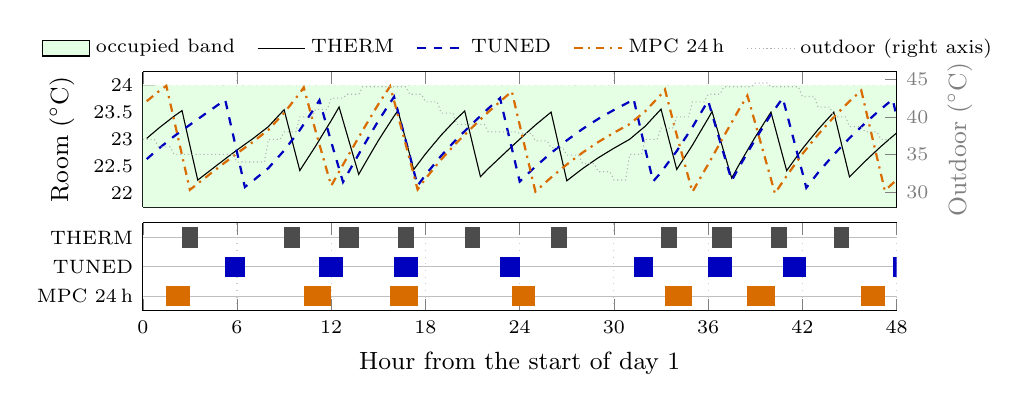
\begin{tikzpicture}
\begin{axis}[
  width=0.92\textwidth, height=3.3cm,
  xmin=0, xmax=48, ymin=21.75, ymax=24.25,
  xtick={0,6,...,48}, xticklabels={,,,,,,,,},
  ytick={22,22.5,23,23.5,24},
  ylabel={Room ($^\circ$C)},
  grid=major, grid style={dotted,gray!40},
  tick label style={font=\scriptsize}, label style={font=\small},
  legend style={font=\scriptsize, at={(0.5,1.02)}, anchor=south,
    legend columns=5, draw=none, fill=none, /tikz/every even column/.append style={column sep=6pt}},
  name=main, axis y line*=left,
]
\addplot[fill=green!10,draw=none,area legend] coordinates{(0,22)(0,24)(48,24)(48,22)}\closedcycle;
\addlegendentry{occupied band}
\addplot[black, thin] coordinates{(0.25,23.018)(0.50,23.081)(0.75,23.142)(1.00,23.204)(1.25,23.261)(1.50,23.317)(1.75,23.374)(2.00,23.430)(2.25,23.481)(2.50,23.532)(2.75,23.209)(3.00,22.887)(3.25,22.567)(3.50,22.248)(3.75,22.305)(4.00,22.361)(4.25,22.417)(4.50,22.473)(4.75,22.529)(5.00,22.584)(5.25,22.640)(5.50,22.695)(5.75,22.749)(6.00,22.804)(6.25,22.856)(6.50,22.908)(6.75,22.960)(7.00,23.011)(7.25,23.068)(7.50,23.124)(7.75,23.180)(8.00,23.236)(8.25,23.315)(8.50,23.393)(8.75,23.471)(9.00,23.548)(9.25,23.266)(9.50,22.984)(9.75,22.704)(10.00,22.425)(10.25,22.538)(10.50,22.650)(10.75,22.762)(11.00,22.874)(11.25,22.993)(11.50,23.113)(11.75,23.231)(12.00,23.349)(12.25,23.474)(12.50,23.598)(12.75,23.348)(13.00,23.099)(13.25,22.849)(13.50,22.601)(13.75,22.354)(14.00,22.482)(14.25,22.607)(14.50,22.732)(14.75,22.856)(15.00,22.979)(15.25,23.093)(15.50,23.206)(15.75,23.318)(16.00,23.430)(16.25,23.532)(16.50,23.260)(16.75,22.989)(17.00,22.719)(17.25,22.441)(17.50,22.538)(17.75,22.635)(18.00,22.731)(18.25,22.819)(18.50,22.906)(18.75,22.992)(19.00,23.079)(19.25,23.156)(19.50,23.233)(19.75,23.310)(20.00,23.387)(20.25,23.456)(20.50,23.525)(20.75,23.220)(21.00,22.916)(21.25,22.613)(21.50,22.312)(21.75,22.386)(22.00,22.460)(22.25,22.529)(22.50,22.597)(22.75,22.666)(23.00,22.734)(23.25,22.802)(23.50,22.869)(23.75,22.937)(24.00,23.003)(24.25,23.069)(24.50,23.135)(24.75,23.200)(25.00,23.265)(25.25,23.325)(25.50,23.385)(25.75,23.444)(26.00,23.504)(26.25,23.185)(26.50,22.867)(26.75,22.551)(27.00,22.236)(27.25,22.292)(27.50,22.348)(27.75,22.404)(28.00,22.459)(28.25,22.510)(28.50,22.560)(28.75,22.610)(29.00,22.660)(29.25,22.704)(29.50,22.749)(29.75,22.793)(30.00,22.837)(30.25,22.878)(30.50,22.920)(30.75,22.961)(31.00,23.002)(31.25,23.063)(31.50,23.124)(31.75,23.185)(32.00,23.245)(32.25,23.324)(32.50,23.403)(32.75,23.481)(33.00,23.559)(33.25,23.278)(33.50,22.999)(33.75,22.722)(34.00,22.445)(34.25,22.558)(34.50,22.670)(34.75,22.782)(35.00,22.894)(35.25,23.018)(35.50,23.142)(35.75,23.265)(36.00,23.387)(36.25,23.514)(36.50,23.266)(36.75,23.019)(37.00,22.773)(37.25,22.529)(37.50,22.286)(37.75,22.418)(38.00,22.550)(38.25,22.674)(38.50,22.798)(38.75,22.922)(39.00,23.044)(39.25,23.160)(39.50,23.275)(39.75,23.390)(40.00,23.504)(40.25,23.232)(40.50,22.961)(40.75,22.691)(41.00,22.422)(41.25,22.524)(41.50,22.625)(41.75,22.725)(42.00,22.826)(42.25,22.916)(42.50,23.005)(42.75,23.094)(43.00,23.183)(43.25,23.264)(43.50,23.344)(43.75,23.424)(44.00,23.503)(44.25,23.203)(44.50,22.903)(44.75,22.605)(45.00,22.308)(45.25,22.381)(45.50,22.453)(45.75,22.525)(46.00,22.597)(46.25,22.666)(46.50,22.734)(46.75,22.802)(47.00,22.869)(47.25,22.932)(47.50,22.995)(47.75,23.057)(48.00,23.119)};
\addlegendentry{THERM}
\addplot[blue!75!black, thick, dashed] coordinates{(0.25,22.636)(0.50,22.699)(0.75,22.763)(1.00,22.826)(1.25,22.885)(1.50,22.943)(1.75,23.001)(2.00,23.059)(2.25,23.112)(2.50,23.165)(2.75,23.217)(3.00,23.270)(3.25,23.322)(3.50,23.374)(3.75,23.425)(4.00,23.477)(4.25,23.528)(4.50,23.579)(4.75,23.630)(5.00,23.680)(5.25,23.730)(5.50,23.406)(5.75,23.084)(6.00,22.763)(6.25,22.441)(6.50,22.120)(6.75,22.176)(7.00,22.231)(7.25,22.291)(7.50,22.351)(7.75,22.410)(8.00,22.470)(8.25,22.552)(8.50,22.633)(8.75,22.714)(9.00,22.795)(9.25,22.890)(9.50,22.984)(9.75,23.078)(10.00,23.172)(10.25,23.282)(10.50,23.391)(10.75,23.499)(11.00,23.607)(11.25,23.724)(11.50,23.466)(11.75,23.209)(12.00,22.953)(12.25,22.705)(12.50,22.459)(12.75,22.213)(13.00,22.343)(13.25,22.471)(13.50,22.599)(13.75,22.726)(14.00,22.852)(14.25,22.976)(14.50,23.099)(14.75,23.221)(15.00,23.343)(15.25,23.455)(15.50,23.566)(15.75,23.677)(16.00,23.787)(16.25,23.514)(16.50,23.242)(16.75,22.970)(17.00,22.701)(17.25,22.423)(17.50,22.146)(17.75,22.244)(18.00,22.343)(18.25,22.432)(18.50,22.520)(18.75,22.609)(19.00,22.697)(19.25,22.776)(19.50,22.855)(19.75,22.933)(20.00,23.011)(20.25,23.083)(20.50,23.153)(20.75,23.224)(21.00,23.294)(21.25,23.364)(21.50,23.433)(21.75,23.502)(22.00,23.571)(22.25,23.635)(22.50,23.699)(22.75,23.763)(23.00,23.452)(23.25,23.142)(23.50,22.834)(23.75,22.527)(24.00,22.222)(24.25,22.291)(24.50,22.360)(24.75,22.429)(25.00,22.497)(25.25,22.560)(25.50,22.624)(25.75,22.687)(26.00,22.749)(26.25,22.808)(26.50,22.866)(26.75,22.924)(27.00,22.982)(27.25,23.035)(27.50,23.087)(27.75,23.140)(28.00,23.192)(28.25,23.239)(28.50,23.286)(28.75,23.333)(29.00,23.379)(29.25,23.421)(29.50,23.462)(29.75,23.503)(30.00,23.544)(30.25,23.582)(30.50,23.620)(30.75,23.658)(31.00,23.696)(31.25,23.755)(31.50,23.438)(31.75,23.123)(32.00,22.810)(32.25,22.517)(32.50,22.225)(32.75,22.308)(33.00,22.391)(33.25,22.490)(33.50,22.589)(33.75,22.687)(34.00,22.785)(34.25,22.896)(34.50,23.007)(34.75,23.117)(35.00,23.227)(35.25,23.350)(35.50,23.472)(35.75,23.594)(36.00,23.715)(36.25,23.466)(36.50,23.218)(36.75,22.971)(37.00,22.726)(37.25,22.482)(37.50,22.239)(37.75,22.372)(38.00,22.503)(38.25,22.628)(38.50,22.752)(38.75,22.876)(39.00,22.999)(39.25,23.115)(39.50,23.230)(39.75,23.345)(40.00,23.460)(40.25,23.562)(40.50,23.663)(40.75,23.764)(41.00,23.491)(41.25,23.213)(41.50,22.937)(41.75,22.662)(42.00,22.389)(42.25,22.106)(42.50,22.200)(42.75,22.292)(43.00,22.385)(43.25,22.469)(43.50,22.553)(43.75,22.636)(44.00,22.719)(44.25,22.796)(44.50,22.872)(44.75,22.948)(45.00,23.024)(45.25,23.094)(45.50,23.163)(45.75,23.232)(46.00,23.301)(46.25,23.366)(46.50,23.431)(46.75,23.496)(47.00,23.560)(47.25,23.620)(47.50,23.680)(47.75,23.739)(48.00,23.424)};
\addlegendentry{TUNED}
\addplot[orange!85!black, thick, dash dot] coordinates{(0.25,23.706)(0.50,23.765)(0.75,23.824)(1.00,23.883)(1.25,23.937)(1.50,23.990)(1.75,23.669)(2.00,23.350)(2.25,23.028)(2.50,22.707)(2.75,22.387)(3.00,22.069)(3.25,22.126)(3.50,22.184)(3.75,22.241)(4.00,22.297)(4.25,22.354)(4.50,22.410)(4.75,22.466)(5.00,22.522)(5.25,22.577)(5.50,22.632)(5.75,22.687)(6.00,22.742)(6.25,22.794)(6.50,22.847)(6.75,22.899)(7.00,22.950)(7.25,23.007)(7.50,23.064)(7.75,23.121)(8.00,23.177)(8.25,23.256)(8.50,23.334)(8.75,23.412)(9.00,23.490)(9.25,23.582)(9.50,23.673)(9.75,23.764)(10.00,23.854)(10.25,23.961)(10.50,23.693)(10.75,23.426)(11.00,23.160)(11.25,22.905)(11.50,22.650)(11.75,22.396)(12.00,22.144)(12.25,22.274)(12.50,22.404)(12.75,22.533)(13.00,22.661)(13.25,22.788)(13.50,22.914)(13.75,23.040)(14.00,23.165)(14.25,23.287)(14.50,23.408)(14.75,23.529)(15.00,23.650)(15.25,23.760)(15.50,23.870)(15.75,23.980)(16.00,23.715)(16.25,23.442)(16.50,23.170)(16.75,22.899)(17.00,22.629)(17.25,22.352)(17.50,22.075)(17.75,22.174)(18.00,22.273)(18.25,22.362)(18.50,22.451)(18.75,22.540)(19.00,22.628)(19.25,22.708)(19.50,22.787)(19.75,22.866)(20.00,22.944)(20.25,23.015)(20.50,23.086)(20.75,23.157)(21.00,23.228)(21.25,23.298)(21.50,23.367)(21.75,23.437)(22.00,23.506)(22.25,23.570)(22.50,23.635)(22.75,23.698)(23.00,23.762)(23.25,23.825)(23.50,23.888)(23.75,23.577)(24.00,23.267)(24.25,22.957)(24.50,22.649)(24.75,22.342)(25.00,22.036)(25.25,22.102)(25.50,22.167)(25.75,22.232)(26.00,22.297)(26.25,22.358)(26.50,22.418)(26.75,22.478)(27.00,22.537)(27.25,22.592)(27.50,22.647)(27.75,22.701)(28.00,22.756)(28.25,22.805)(28.50,22.854)(28.75,22.902)(29.00,22.951)(29.25,22.994)(29.50,23.037)(29.75,23.080)(30.00,23.123)(30.25,23.163)(30.50,23.203)(30.75,23.243)(31.00,23.283)(31.25,23.343)(31.50,23.402)(31.75,23.462)(32.00,23.521)(32.25,23.599)(32.50,23.676)(32.75,23.753)(33.00,23.830)(33.25,23.922)(33.50,23.640)(33.75,23.360)(34.00,23.080)(34.25,22.816)(34.50,22.553)(34.75,22.292)(35.00,22.031)(35.25,22.159)(35.50,22.287)(35.75,22.414)(36.00,22.540)(36.25,22.670)(36.50,22.800)(36.75,22.929)(37.00,23.058)(37.25,23.187)(37.50,23.315)(37.75,23.443)(38.00,23.570)(38.25,23.690)(38.50,23.809)(38.75,23.554)(39.00,23.300)(39.25,23.040)(39.50,22.782)(39.75,22.525)(40.00,22.269)(40.25,22.002)(40.50,22.110)(40.75,22.218)(41.00,22.326)(41.25,22.428)(41.50,22.529)(41.75,22.630)(42.00,22.731)(42.25,22.821)(42.50,22.911)(42.75,23.001)(43.00,23.090)(43.25,23.171)(43.50,23.252)(43.75,23.332)(44.00,23.412)(44.25,23.486)(44.50,23.559)(44.75,23.632)(45.00,23.705)(45.25,23.771)(45.50,23.838)(45.75,23.904)(46.00,23.595)(46.25,23.285)(46.50,22.976)(46.75,22.669)(47.00,22.363)(47.25,22.054)(47.50,22.120)(47.75,22.186)(48.00,22.252)};
\addlegendentry{MPC $24\,$h}
\addlegendimage{gray!60, thin, densely dotted}\addlegendentry{outdoor (right axis)}
\end{axis}
\begin{axis}[
  width=0.92\textwidth, height=3.3cm, at={(main.south west)}, anchor=south west,
  xmin=0, xmax=48, ymin=28, ymax=46,
  axis y line*=right, axis x line=none,
  ytick={30,35,40,45}, ylabel={Outdoor ($^\circ$C)},
  tick label style={font=\scriptsize, gray}, label style={font=\small, gray},
]
\addplot[gray!60, thin, densely dotted] coordinates{(0.00,37.000)(0.25,37.000)(0.50,37.000)(0.75,37.000)(1.00,36.000)(1.25,36.000)(1.50,36.000)(1.75,36.000)(2.00,35.000)(2.25,35.000)(2.50,35.000)(2.75,35.000)(3.00,35.000)(3.25,35.000)(3.50,35.000)(3.75,35.000)(4.00,35.000)(4.25,35.000)(4.50,35.000)(4.75,35.000)(5.00,35.000)(5.25,35.000)(5.50,35.000)(5.75,35.000)(6.00,34.000)(6.25,34.000)(6.50,34.000)(6.75,34.000)(7.00,34.000)(7.25,34.000)(7.50,34.000)(7.75,34.000)(8.00,37.000)(8.25,37.000)(8.50,37.000)(8.75,37.000)(9.00,38.000)(9.25,38.000)(9.50,38.000)(9.75,38.000)(10.00,40.000)(10.25,40.000)(10.50,40.000)(10.75,40.000)(11.00,41.000)(11.25,41.000)(11.50,41.000)(11.75,41.000)(12.00,42.500)(12.25,42.500)(12.50,42.500)(12.75,42.500)(13.00,43.000)(13.25,43.000)(13.50,43.000)(13.75,43.000)(14.00,44.000)(14.25,44.000)(14.50,44.000)(14.75,44.000)(15.00,44.000)(15.25,44.000)(15.50,44.000)(15.75,44.000)(16.00,44.000)(16.25,44.000)(16.50,44.000)(16.75,44.000)(17.00,43.000)(17.25,43.000)(17.50,43.000)(17.75,43.000)(18.00,42.000)(18.25,42.000)(18.50,42.000)(18.75,42.000)(19.00,40.500)(19.25,40.500)(19.50,40.500)(19.75,40.500)(20.00,39.000)(20.25,39.000)(20.50,39.000)(20.75,39.000)(21.00,39.000)(21.25,39.000)(21.50,39.000)(21.75,39.000)(22.00,38.000)(22.25,38.000)(22.50,38.000)(22.75,38.000)(23.00,38.000)(23.25,38.000)(23.50,38.000)(23.75,38.000)(24.00,37.800)(24.25,37.800)(24.50,37.800)(24.75,37.800)(25.00,36.800)(25.25,36.800)(25.50,36.800)(25.75,36.800)(26.00,35.900)(26.25,35.900)(26.50,35.900)(26.75,35.900)(27.00,34.900)(27.25,34.900)(27.50,34.900)(27.75,34.900)(28.00,33.800)(28.25,33.800)(28.50,33.800)(28.75,33.800)(29.00,32.700)(29.25,32.700)(29.50,32.700)(29.75,32.700)(30.00,31.600)(30.25,31.600)(30.50,31.600)(30.75,31.600)(31.00,35.000)(31.25,35.000)(31.50,35.000)(31.75,35.000)(32.00,37.000)(32.25,37.000)(32.50,37.000)(32.75,37.000)(33.00,38.500)(33.25,38.500)(33.50,38.500)(33.75,38.500)(34.00,40.000)(34.25,40.000)(34.50,40.000)(34.75,40.000)(35.00,42.000)(35.25,42.000)(35.50,42.000)(35.75,42.000)(36.00,43.000)(36.25,43.000)(36.50,43.000)(36.75,43.000)(37.00,44.000)(37.25,44.000)(37.50,44.000)(37.75,44.000)(38.00,44.000)(38.25,44.000)(38.50,44.000)(38.75,44.000)(39.00,44.500)(39.25,44.500)(39.50,44.500)(39.75,44.500)(40.00,44.000)(40.25,44.000)(40.50,44.000)(40.75,44.000)(41.00,44.000)(41.25,44.000)(41.50,44.000)(41.75,44.000)(42.00,42.700)(42.25,42.700)(42.50,42.700)(42.75,42.700)(43.00,41.300)(43.25,41.300)(43.50,41.300)(43.75,41.300)(44.00,40.000)(44.25,40.000)(44.50,40.000)(44.75,40.000)(45.00,38.700)(45.25,38.700)(45.50,38.700)(45.75,38.700)(46.00,38.000)(46.25,38.000)(46.50,38.000)(46.75,38.000)(47.00,37.000)(47.25,37.000)(47.50,37.000)(47.75,37.000)};
\end{axis}
\begin{axis}[
  at={(main.south west)}, anchor=north west, yshift=-2mm,
  width=0.92\textwidth, height=2.7cm, xmin=0, xmax=48, ymin=0, ymax=3,
  xtick={0,6,...,48}, xlabel={Hour from the start of day 1},
  ytick={0.5,1.5,2.5}, yticklabels={MPC $24\,$h,TUNED,THERM},
  y tick style={draw=none}, axis y line*=left,
  grid=none, xmajorgrids, grid style={dotted,gray!40},
  tick label style={font=\scriptsize}, label style={font=\small},
]
\addplot[draw=gray!50,thin] coordinates{(0,2.5)(48,2.5)};
\fill[black!70] (axis cs:2.5,2.15) rectangle (axis cs:3.5,2.85);
\fill[black!70] (axis cs:9,2.15) rectangle (axis cs:10,2.85);
\fill[black!70] (axis cs:12.5,2.15) rectangle (axis cs:13.75,2.85);
\fill[black!70] (axis cs:16.25,2.15) rectangle (axis cs:17.25,2.85);
\fill[black!70] (axis cs:20.5,2.15) rectangle (axis cs:21.5,2.85);
\fill[black!70] (axis cs:26,2.15) rectangle (axis cs:27,2.85);
\fill[black!70] (axis cs:33,2.15) rectangle (axis cs:34,2.85);
\fill[black!70] (axis cs:36.25,2.15) rectangle (axis cs:37.5,2.85);
\fill[black!70] (axis cs:40,2.15) rectangle (axis cs:41,2.85);
\fill[black!70] (axis cs:44,2.15) rectangle (axis cs:45,2.85);
\addplot[draw=gray!50,thin] coordinates{(0,1.5)(48,1.5)};
\fill[blue!75!black] (axis cs:5.25,1.15) rectangle (axis cs:6.5,1.85);
\fill[blue!75!black] (axis cs:11.25,1.15) rectangle (axis cs:12.75,1.85);
\fill[blue!75!black] (axis cs:16,1.15) rectangle (axis cs:17.5,1.85);
\fill[blue!75!black] (axis cs:22.75,1.15) rectangle (axis cs:24,1.85);
\fill[blue!75!black] (axis cs:31.25,1.15) rectangle (axis cs:32.5,1.85);
\fill[blue!75!black] (axis cs:36,1.15) rectangle (axis cs:37.5,1.85);
\fill[blue!75!black] (axis cs:40.75,1.15) rectangle (axis cs:42.25,1.85);
\fill[blue!75!black] (axis cs:47.75,1.15) rectangle (axis cs:48,1.85);
\addplot[draw=gray!50,thin] coordinates{(0,0.5)(48,0.5)};
\fill[orange!85!black] (axis cs:1.5,0.15) rectangle (axis cs:3,0.85);
\fill[orange!85!black] (axis cs:10.25,0.15) rectangle (axis cs:12,0.85);
\fill[orange!85!black] (axis cs:15.75,0.15) rectangle (axis cs:17.5,0.85);
\fill[orange!85!black] (axis cs:23.5,0.15) rectangle (axis cs:25,0.85);
\fill[orange!85!black] (axis cs:33.25,0.15) rectangle (axis cs:35,0.85);
\fill[orange!85!black] (axis cs:38.5,0.15) rectangle (axis cs:40.25,0.85);
\fill[orange!85!black] (axis cs:45.75,0.15) rectangle (axis cs:47.25,0.85);
\end{axis}
\end{tikzpicture}
\caption{A two-day operating trace: the held-out Riyadh week with the highest mean outdoor temperature, days~1--2, fixed before the traces were drawn (day~0 is not shown). It is the held-out week in which TUNED's saving is lowest ($11.1\%$); the MPC margin over it there is $6.3$ points. Upper: room temperature at the end of each $15$-min step under THERM (unshifted), TUNED and the $24\,$h MPC (perfect forecast), with the occupied band $[22,24]\,^\circ$C shaded and the outdoor temperature (31.6--44.5$\,^\circ$C) on the right axis. Lower: cooling command (filled: on). THERM, TUNED and MPC issue 10, 8 and 7 on-commands over the two days and 34, 27 and 23 over the week. TUNED's switch points (23.71/22.36$\,^\circ$C) widen THERM's $1\,^\circ$C deadband, so it cycles less; MPC uses the full band (22.00--23.99$\,^\circ$C).}
\label{fig:traces}
\end{figure*}


\emph{The tuned thermostat.} Commissioning the two switch points avoids
$22.8$, $24.2$ and $21.7\%$ of on-commands and saves $12.5$, $13.6$ and
$12.4\%$ of cost in Riyadh, Jeddah and Taif, in every held-out
window of every city (family F1: Hodges--Lehmann $+12.6$, $+13.7$ and
$+11.8$ points, Holm-adjusted $p=0.047$ in each city), with no model, no
forecast and no state beyond the zone temperature. The mechanism is a wider
deadband: the fitted switch points (Section~\ref{subsec:rules}) widen THERM's
$1\,^\circ$C deadband to $1.35$, $1.36$ and $1.32\,^\circ$C, close to the
widest that the band and the $15$-min excursion admit (Remark~\ref{rem:rc}),
and the share of on-commands avoided is roughly
$1-\delta_{\mathrm{THERM}}/\delta_{\mathrm{TUNED}}$. The saving is therefore
a statement about the comparator's assumed $1\,^\circ$C deadband as much as
about tuning (Section~\ref{subsec:abl_component}). At the charges the wear
derivation supports, $0.025$ and $0.114\,\SAR$, it saves $3.8$--$11.0\%$,
$4.3$--$12.0\%$ and $3.9$--$10.9\%$. These switch points are fitted on a
$0.01\,^\circ$C grid. A real thermostat sets its thresholds in steps of about
$0.1\,^\circ$C, and on that grid the tuned rule avoids $10.5$, $13.2$ and
$14.7\%$ of on-commands and saves $5.7$, $7.4$ and $8.4\%$
(at $23.6/22.4\,^\circ$C in every city, which in Riyadh is the guard
hysteresis, so on that grid the guard's shortfall F4 vanishes in Riyadh and the
guard exceeds TUNED in Taif); under a per-window $0.03\,$K admission criterion
it saves $9.7$, $12.2$ and $4.0\%$, $8.4$ points less in Taif, where the guard
then exceeds it (Supplementary Table~S2). The headline TUNED figures are
therefore an upper estimate of what a commissioned thermostat delivers. Any
claim for a learned or model-based controller is measured against TUNED, not
THERM.

\emph{Taif.} The lower load does not leave less to win in percentage terms:
TUNED saves $12.4\%$ against a bracket of $16.7$--$21.0\%$, the widest of the
three, with the lowest lower end and the highest upper end. The $24\,$h controller's $16.9\%$
uses the simulator terminal; under $V_N$ its equalised saving is $16.3\%$,
below CLV's $16.5\%$.

Under the schedule announced for January 2027 ($0.21\,\SAR/\kWh$) TUNED saves
$11.6$, $12.7$ and $11.6\%$, and $18.6$, $19.9$ and $18.0\%$ at the pre-2018
first-block price, while the on-commands it avoids are unchanged, because a
higher energy price dilutes a saving whose mechanism is a fixed charge per
on-command.

\emph{Occupancy setback.} With the dwelling empty from 08:00 to 14:00 on
working days and an away limit of $30\,^\circ$C, a tuned setback rule
(TUNED-SB, with a fitted pre-arrival lead of $2$, $1.25$ and $1\,$h) saves
$18.6$, $20.1$ and $17.0\%$ ($\Delta\tilde T=+0.058$, $+0.027$, $+0.001\,$K),
and a $24\,$h receding-horizon controller with the timetable (MPC-SB) saves
$24.0$, $23.3$ and $23.2\%$ ($\Delta\tilde T=-0.030$, $-0.019$, $-0.076\,$K),
against setback bounds of $27.8$, $27.6$ and $28.8\%$ and raw setback
clairvoyant schedules of $25.3$, $25.3$ and $23.9\%$. Both are compared with
THERM without setback, equalised on the occupied steps, so the saving includes
letting the empty house float. The pre-arrival lead is not pre-cooling: it is
the latest start that meets the $24\,^\circ$C ceiling at arrival, and no
cooling is banked beyond it.

Switching off at departure
and on at arrival with no lead (MANUAL) is a reference, not an admitted arm:
it leaves $21.8$, $9.8$ and $3.3$ occupied degree-hours above the band after
arrival, and its nominal saving ($14.6$, $13.0$ and $13.7\%$) is bought with
that over-temperature; THERM with the setback away limit
coincides with it, because the away limit never binds (the empty zone peaks at
$24.8$--$25.9\,^\circ$C). The mechanism is on-commands avoided while the house
is empty: TUNED-SB avoids $33.6$, $35.0$ and $29.2\%$ of the equalised
baseline's on-commands while energy moves by $-0.2$, $+0.6$ and $-0.8\%$, and
MPC-SB avoids $42.3$, $39.7$ and $39.3\%$ with energy $+0.6$, $+2.1$ and
$+3.3\%$ (vacation weeks: Supplementary Section~S8). MPC-SB plans on the timetable it is given, and the model has no
internal gains and a constant capacity, both of which flatter the recovery.


\subsection{Where the Receding-Horizon Margin Comes From}
\label{subsec:ladder}

The receding-horizon controller differs from TUNED in three ways at once: it
has an exact model of the plant, it sees a forecast, and it plans over a
horizon. The arms of Table~\ref{tab:main} form a ladder that separates them:
THERM, TUNED, the D1 shield (an exact one-step model with no horizon), MPC at
$0.25$, $1$, $2$, $6$, $24$ and $48\,$h with a perfect forecast, MPC with a
persistence forecast, MPC confined to the rule set, E2-PPO, and finally CLV
and the bound.

\emph{Against TUNED.} With a perfect in-horizon forecast the $24\,$h
controller avoids $33.3$, $32.0$ and $29.8\%$ of on-commands against TUNED's
$22.8$, $24.2$ and $21.7\%$, and its cost saving exceeds TUNED's in every
held-out window of every city, by
Hodges--Lehmann estimates of $+6.0$, $+4.2$ and $+4.6$ points (family F2,
$95.3\%$ intervals $[+3.8,+7.5]$, $[+3.8,+5.3]$ and $[+2.0,+8.0]$). With a persistence forecast the difference is $-0.1$,
$+0.9$ and $-1.9$ points, with intervals that include zero and pooled
differences under $3$ points: not resolved (F3). With the one imperfect
forecast tested, the margin over the tuned thermostat is therefore not
resolved; forecasts between persistence and perfect were not tested. The
persistence arms run $0.09$, $0.07$ and $0.09\,$K cooler than TUNED, in
Riyadh and Taif at the $0.10\,$K fallback, which by the comfort-offset caveat
penalises them; the back-off knob is tried only when no $\lambda$ is
admissible at $0.10\,$K, so it was not applied to these cells.

\emph{Horizon and model.} The horizon sweep is descriptive
(Table~\ref{tab:main}, with its back-off and fallback marks). Savings rise
with the horizon up to $6\,$h, and differences of less than $3$ points beyond
it are not resolved; the Taif $48\,$h cell, fitted at the fallback and
$0.09\,$K warmer than THERM, exceeds the clairvoyant lower end. The
$0.25\,$h controller saves at most $2\%$ and costs more than the baseline in
Riyadh ($-3.9\%$). The one-step D1 shield on a latch saves
$14.0$, $13.5$ and $12.4\%$, within $1.4$ points of TUNED in every city, while
the $24\,$h controller exceeds it by $4.3$, $4.6$ and $4.5$ points: an exact
one-step model reaches the tuned thermostat, and the margin beyond it needs
the horizon and the forecast.

\emph{Forecast.} At $6\,$h a persistence forecast costs $0.7$ points in
Riyadh and $1.9$ in Taif, leaving $14.4$ and $14.0\%$, $1.9$ and $1.6$ points
above TUNED (not resolved); in Jeddah no multiplier or back-off is admissible
at $6\,$h. At $24\,$h it costs $5.5$, $3.4$ and $6.2$ points, partly at a
cooler matched comfort (Table~\ref{tab:main}). Both modes plan on the plant's own model with the
exact state, so neither measures model mismatch.

\emph{Thermal capacity.} The single-node capacity is assumed, and the capacity
effective at the cycle period is below the ISO~13786 value
(Remark~\ref{rem:rc}). In Riyadh, refitted at each capacity, TUNED saves
$-2.8$, $12.5$, $16.0$ and $15.8\%$ at $2{,}400$, $4{,}800$, $7{,}200$ and
$9{,}600\,\text{kJ/K}$, and the $24\,$h controller $12.2$, $18.3$, $19.8$ and
$16.2\%$, so its margin over TUNED is $15.0$, $5.7$, $3.8$ and $0.4$ points
(Table~\ref{tab:sensitivity}); in Jeddah and Taif TUNED moves from $-1.4$ and
$-1.3\%$ to $15.8$ and $16.0\%$ ($16.7$ and $17.7\%$ at $7{,}200\,\text{kJ/K}$).
The on-commands TUNED avoids rise monotonically with capacity in every city (Riyadh $-4.0$,
$22.8$, $34.6$ and $39.8\%$). Its cost saving does not: the $7{,}200$ and
$9{,}600\,\text{kJ/K}$ figures differ by less than $3$ points in every city,
and at $7{,}200\,\text{kJ/K}$ TUNED sits $0.033$, $0.040$ and $0.121\,$K warmer
than THERM against $-0.019$, $+0.029$ and $-0.018\,$K at $9{,}600$, so their
order is not resolved. The planner's drop from $19.8$ to $16.2\%$ comes with a
$0.044\,$K cooler matched mean and $2.5\%$ more electricity at
$9{,}600\,\text{kJ/K}$, while the on-commands it avoids barely move ($42.4$
and $40.7\%$). On the light plant tested ($2{,}400\,\text{kJ/K}$) the
commissioned thermostat does not beat a $1\,^\circ$C deadband: each on-step
overshoots by $0.75\,$K, TUNED's fitted deadband shrinks to $0.96\,^\circ$C,
and THERM's own fails~\eqref{eq:deadband_condition} narrowly; THERM's
self-score under Rule~C was not computed there, so the small negative savings
are not resolved from zero. On a heavy plant TUNED captures almost all of what
the planner does. The ordering and its size therefore depend on the assumed
capacity, and because the capacity acting over a cycle is probably below the
reference (Remark~\ref{rem:rc}), the reference results lean towards the end
favourable to TUNED.

\emph{Robustness of the comfort device.} The fitted multipliers of the $6$ and
$24\,$h perfect-forecast controllers lie at $\lambda/\lambda^\ast=1.002$--$1.024$.
In the following cells the fitted multiplier lies far above $\lambda^\ast$:
$\lambda/\lambda^\ast=1.226$ and $4.577$ at $48\,$h in Riyadh and Jeddah,
$13.094$, $2.326$ and $6.218$ for the $24\,$h persistence controller, and
$2.089$ and $1.801$ in rules at $24\,$h in Riyadh and Taif. Near
$\lambda^\ast$ the saving is sensitive to $\lambda$: neighbouring admissible multipliers
move the Riyadh $24\,$h saving by $1.4$--$1.8$ points. Runs at fixed
$\lambda^\ast\cdot\{0.99,1.01,1.05\}$ are not comfort-matched and are given,
with their $\Delta\tilde T$, in Supplementary Table~S2 only; grid refinement is
reported in Section~\ref{subsec:compete}.

\emph{Inside the rules.} Confined to the training rule set
($23.80/22.40\,^\circ$C) the $24\,$h controller saves $11.6$, $14.1$ and
$10.0\%$, below relaxed bounds in those rules of $14.9$, $15.6$ and $16.2\%$.
Confined to each city's
\emph{fitted} guard thresholds, the rules the guard hysteresis itself uses, it
saves $6.7$, $4.4$ and $10.5\%$ against $5.7$, $7.6$ and $11.0\%$ for the
guard: it does not beat the guard by a resolved margin in any city, and in
Jeddah it falls $3.3$ points short at a $0.03\,$K warmer mean, in a cell fitted
at the $0.10\,$K fallback with $\lambda/\lambda^\ast=0.60$. Inside the wider
training rules, whose on threshold is $0.14$--$0.20\,$K higher, the $24\,$h
controller exceeds the fitted guard by $5.9$ and $6.4$ points in Riyadh and
Jeddah despite a $0.10$ and $0.04\,$K cooler mean, which penalises it; this
compares different rule sets. Replacing the guard's fixed margins by the D1
shield's one-step prediction lifts the latch to TUNED's level ($14.0$, $13.5$
and $12.4\%$). Applied to the trained PPO policies in place of their rule
layer, D1 gives $12.8$--$14.1$ and $11.2$--$13.5\%$ in Riyadh and Jeddah, the
latch's level, but $8.0$--$12.0\%$ in Taif, below the latch's $12.4\%$, and
for three of the five seeds below their own rule-layer results (seed~42: $8.0$
against $8.6\%$).
Inside the guard's own fitted thresholds, then, neither lookahead nor learning
adds a resolved margin, and the one-step shield sets the level
(Remark~\ref{rem:cor_scope}).

\subsection{Multi-Zone Dwellings}
\label{subsec:multizone}
\label{subsec:res_all}

%% Gate (RULING §12.1): J-MZ by Sat 14 Nov 20:00. If missed, replace this
%% subsection by one body sentence pointing to Table S-MZ and the repository.
Whether the single-zone ordering survives in a dwelling of several rooms is
tested in Riyadh for four layouts: the single zone, a $1\times2$ row, a
$2\times2$ grid and a $1\times4$ row, each with the glazed faces at the fixed
azimuths of Table~S-MZ and $\lij=12.5\,$W/K, with $35\,$W/K as a sensitivity.
Every room has its own unit, so there is no shared capacity limit; rooms are
coupled only through the shared walls. The arms are THERM, TUNED, the guard
hysteresis and a multi-zone receding-horizon controller, all under the
protocol of Section~\ref{subsec:protocol} applied to the dwelling's mean
occupied temperature, with each room's mean and the spread between rooms
reported beside it. The multi-zone controller is a non-cooperative distributed
MPC with one-step-delayed plan exchange \citep{Scattolini2009} (Supplementary
Section~S7), with no optimality guarantee and no bound, because the joint
dynamic programme is intractable (Section~\ref{subsec:abl_cost}).

With rules alone, TUNED on the dwelling mean saves $12.5\%$ in the single
zone, $12.4\%$ in the $1\times2$ row, $11.7\%$ in the $2\times2$ grid and
$13.6\%$ in the $1\times4$ row ($12.2$, $12.9$ and $13.3\%$ at
$\lij=35\,$W/K), and the guard hysteresis $5.7$, $7.2$, $8.3$ and $7.7\%$; the
mean spread of the room temperatures is $0.03$--$0.08\,$K. The multi-zone
receding-horizon controller ($24\,$h, perfect forecast) saves $16.0$, $15.9$ and
$15.7\%$ ($15.8$, $16.1$ and $16.1\%$ at $\lij=35\,$W/K), avoiding
$28$--$32\%$ of the equalised baseline's on-commands with electricity within
$\pm0.7\%$; on the $1\times1$ instance it reproduces the single-zone $18.3\%$
exactly (Table~S-MZ). Its margin over TUNED is not tested for significance
in the multi-zone layouts. Every room has the
same band and timetable, so the rooms' mean temperatures differ by only
$0.03$--$0.08\,$K and little heat crosses a wall: the study tests whether the single-zone ordering transfers to a coupled
dwelling, not what coordination is worth.

\section{State-of-the-Art Comparison and Ablation Study}
\label{sec:analysis}

This section compares the figures with published ones, ablates the rule layer
and the learned component, gathers the sensitivities, and reports
computational cost.

\subsection{State-of-the-Art Comparison}
\label{subsec:sota}

Published RL-based HVAC studies differ in control type, building type,
baseline and climate; Table~\ref{tab:sota} records the basis of each figure.

\begin{table*}[t]
\centering
\caption{State-of-the-art comparison. The ``Basis'' column is essential
for interpreting saving figures.}
\label{tab:sota}
\setlength{\tabcolsep}{6pt}
\begin{tabularx}{\textwidth}{
>{\raggedright\arraybackslash}X
>{\centering\arraybackslash}X
>{\raggedright\arraybackslash}p{0.30\linewidth}
>{\centering\arraybackslash}X
>{\raggedleft\arraybackslash}p{0.22\linewidth}
}
\toprule
Reference & Year & Method & Saving & Basis \\
\midrule
\citep{Azuatalam2020} & 2020 & RL, whole commercial building & 22\% & vs.\ handcrafted rule \\
\citep{Du2021b}        & 2021 & DDPG, multi-zone residential & 15\% & vs.\ DQN \\
\citep{Biemann2021}    & 2021 & SAC/TD3, continuous    & $>$10\% & vs.\ rule-based \\
\citep{Wang2024DRL}    & 2024 & DRL, continuous VAV    & 37\%$^{a}$ & vs.\ rule-based \\
\citep{Solinas2024}    & 2024 & Online RL, white-box   & 65\%$^{b}$ & vs.\ no control \\
\citep{Xue2025}        & 2025 & GA-MADDPG hybrid       & 6.7\%  & vs.\ rule-based \\
\midrule
\textbf{This work} & 2026 & TUNED / MPC-$24\,$h / bracket, Riyadh & $12.5$ / $18.3$ / $18.0$--$20.0\%$ & vs.\ thermostat at equal mean, held out; on-commands priced at $0.15\,\SAR$, electricity ${\approx}0$ \\
\bottomrule
\multicolumn{5}{l}{\footnotesize
$^{a}$Continuous VAV modulation in a simulated office: different hardware
and building type.}\\
\multicolumn{5}{l}{\footnotesize
$^{b}$Relative to a no-HVAC baseline; saving vs.\ thermostat is
substantially lower.}
\end{tabularx}
\end{table*}

\citet{Xue2025}, whose protocol is closest to this one (a rule-based
comparator and a cost objective), report $6.7\%$. The figures here differ in
three ways. Two lower them: the comparator is shifted to the arm's own mean
temperature, and every figure is held out. One raises them: the saving is
priced on on-commands at the $0.15\,\SAR$ reference, above the derived range,
at which TUNED would save $3.8$--$11.0\%$ in Riyadh. Electricity is about
unchanged here, whereas the published figures are energy or cost savings. The larger published figures differ in scope, not degree, as the
notes record.

\subsection{Component Ablation and Sensitivity}
\label{subsec:abl_component}

\emph{The rule layer.} Without R1 and R2, PPO trained on the same reward with
a linear comfort penalty yields an admissible ceiling for one of five seeds in
Riyadh, which then saves $-3.5\%$, and for none of the five in Jeddah or Taif.
That ceiling, $23.50\,^\circ$C, is the lower edge of the search grid, so the
null for the other nine runs may partly reflect the grid's range. This shows
that this configuration fails to optimise without the rules; it does not show
that a learner needs them.

\emph{The learned component.} Under the rule layer, PPO on the cost-only
reward reproduces the guard hysteresis in Riyadh and Jeddah: four of five
seeds in each reproduce the guard's pooled saving to $10^{-5}$ ($5.745$ and
$7.624\%$) and the fifth differs by less than $0.004$ points. In Taif it does
not: one seed equals the guard ($11.0\%$) and the other four, at fitted
ceilings of $23.84$ or $23.86\,^\circ$C, save $1.0$--$2.4$ points less. Inside
the rules hold is within $0.4$, $1.4$ and $2.3\%$ of the $\lambda=0$
dynamic-programming optimum in Riyadh, Jeddah and Taif (E1), so it is nearly
optimal for the cost-only reward. E2, trained in Riyadh only with three seeds,
a comfort term and a forecast, is not selected by Rule~A and not
comfort-matched; it stays within $0.16$ on-commands per day and $2.6\%$ of
cost of the hold policy at the training rules. Because its multiplier sits near
$\lambda^\ast$, where the $\lambda$ term is flat in comfort, and hold is within
$0.4\%$ of the reward's optimum in Riyadh, E2 is consistent with, not evidence
for, a learning null; its savings are not tabulated. Applying the exact
one-step shield D1 in place of the five trained policies' rule layer gives
$12.8$--$14.1$ and $11.2$--$13.5\%$ in Riyadh and Jeddah, the latch's level,
and $8.0$--$12.0\%$ in Taif, below it; the level is set by the shield, not by
the policies, which on their tuning weeks already sit within $0.9\%$ of the
hold policy's training cost except one Taif seed ($1.4\%$;
Section~\ref{subsec:reward}).

\emph{The price of the guarantee.} Compared with TUNED, which has no guard
bands, the guard hysteresis costs $6.8$ and $6.0$ points pooled in Riyadh and
Jeddah (Hodges--Lehmann $6.6$ and $6.0$), in every window (family F4); in Taif
the difference, $-1.4$ points pooled, is not resolved, with the guard
$0.05\,$K warmer than TUNED. On the $0.1\,^\circ$C hardware grid the Riyadh
difference vanishes, and under the per-window admission criterion the guard
exceeds TUNED in Taif (Section~\ref{subsec:consumption}). What the guards buy
is a guarantee under the nominal plant parameters: nothing in TUNED's
construction prevents an over-temperature or a cooling step below the band on
unseen weather (it records the latter in Jeddah and Taif), whereas R1 and R2
exclude both by construction.

\begin{table*}[t]
\centering
\caption{Sensitivity of the pooled equalised saving, Riyadh, seven held-out
windows; descriptive, no tests. (a)~Tariff schedule at $\csw=0.15\,\SAR$.
(b)~Charge per on-command at the tariff in force; the derived range is
$0.025$--$0.114\,\SAR$. (c)~THERM's deadband at a fixed $[22,24]\,^\circ$C
band; admissibility by~\eqref{eq:deadband_condition}; the comparator is
sampled at $15\,$min. (d)~Thermal capacity, every arm refitted by Rule~A.
Every TUNED and MPC cell is fitted at pooled $0.03\,$K; $B^\ast$ under $V_N$.
On-command share: $\csw f_s/J$ of THERM. Bold: reference setting. At
$2{,}400\,\text{kJ/K}$ THERM's $1\,^\circ$C deadband fails~\eqref{eq:deadband_condition}
narrowly. TUNED is refitted at every charge; its switch points stay at
$23.71/22.36\,^\circ$C for every $\csw>0$ because the comfort limits bind, and
move to $23.54/22.39\,^\circ$C at $\csw=0$.}
\label{tab:sensitivity}
\setlength{\tabcolsep}{3pt}
\small
\begin{tabular*}{\textwidth}{@{\extracolsep{\fill}}lrrrr@{}}
\toprule
Setting & THERM on-command share & TUNED & MPC-$24\,$h & $B^\ast$ \\
\midrule
\multicolumn{5}{@{}l}{\emph{(a) Tariff} ($\SAR/\kWh$)}\\
$0.05$ (pre-2018) & $81.5\%$ & $18.6$ & --- & $\le29.6$ \\
$\mathbf{0.18}$ (in force) & $55.0\%$ & $12.5$ & $18.3$ & $\le20.0$ \\
$0.21$ (2027) & $51.2\%$ & $11.6$ & --- & $\le18.6$ \\
\multicolumn{5}{@{}l}{\emph{(b) Charge per on-command} ($\SAR$)}\\
$0$ & $0.0\%$ & $0.0$ & --- & --- \\
$0.025$ & $16.9\%$ & $3.8$ & $5.7$ & $\le6.3$ \\
$0.05$ & $29.0\%$ & $6.6$ & --- & --- \\
$0.10$ & $44.9\%$ & $10.2$ & --- & --- \\
$0.114$ & $48.2\%$ & $11.0$ & $16.1$ & $\le17.5$ \\
$\mathbf{0.15}$ & $55.0\%$ & $12.5$ & $18.3$ & $\le20.0$ \\
$0.20$ & $62.0\%$ & $14.1$ & --- & --- \\
$0.30$ & $71.0\%$ & $16.2$ & --- & --- \\
$0.60$ & $83.0\%$ & $18.9$ & --- & --- \\
\multicolumn{5}{@{}l}{\emph{(c) THERM deadband} ($^\circ$C; THERM on-commands/day)}\\
$0.50$ ($7.37$) & --- & $40.2$ & --- & --- \\
$0.75$ ($5.22$) & --- & $23.4$ & --- & --- \\
$\mathbf{1.00}$ ($4.10$) & --- & $12.5$ & $18.3$ & --- \\
$1.25$ ($3.45$) & --- & $5.7$ & --- & --- \\
$1.50$ & \multicolumn{4}{c}{inadmissible by~\eqref{eq:deadband_condition}} \\
\multicolumn{5}{@{}l}{\emph{(d) Thermal capacity} (kJ/K)}\\
$2{,}400$ (THERM $7.43$/day) & --- & $-2.8$ & $12.2$ & --- \\
$\mathbf{4{,}800}$ ($4.10$/day) & $55.0\%$ & $12.5$ & $18.3$ & $\le20.0$ \\
$7{,}200$ ($2.94$/day) & --- & $16.0$ & $19.8$ & $\le20.0$ \\
$9{,}600$ ($2.24$/day) & --- & $15.8$ & $16.2$ & --- \\
\bottomrule
\end{tabular*}
\end{table*}

\emph{Sensitivities.} Table~\ref{tab:sensitivity} gathers the economic and
physical parameters. The tariff and the charge per on-command move the
percentage through the share of the baseline's cost that on-commands carry,
as Remark~\ref{rem:csw} predicts. The comparator's deadband moves the saving
most, from $40.2\%$ at $0.5\,^\circ$C to $5.7\%$ at $1.25\,^\circ$C, because it
sets how often the baseline cycles: the reported figure is a statement about a
pair, controller and comparator. TUNED was refitted at every charge; its
switch points do not move for any positive charge, because the comfort limits
bind before the charge does. The adopted $\deadband=1\,^\circ$C is assumed,
not measured. It sits near the upper end of the interval
$[0.375,1.25]\,^\circ$C admissible when the comparator is sampled at
$15\,$min, a cap that a continuously sensing thermostat does not share, so an
installed thermostat could have a wider deadband, against which TUNED saves
less ($5.7\%$ against $1.25\,^\circ$C). Measuring the installed stock's deadband
is the field test most likely to confirm or overturn these results.

\subsection{Actuation Step}
\label{subsec:timestep}

Every figure above is tied to the $15$-min actuation step.
Table~\ref{tab:timestep} and Fig.~\ref{fig:timestep} repeat TUNED, the $24\,$h controller and the bound
at $5$ and $30\,$min, each arm refitted by Rule~A. At $5\,$min the tuned
thermostat avoids $43.1$, $41.9$ and $43.0\%$ of on-commands, against $22.8$,
$24.2$ and $21.7\%$ at $15\,$min, with electricity within $1\%$ of the
equalised baseline's; its cost saving doubles to about $25\%$ and reaches
$92\%$ of the Riyadh bound. Its difference from the Riyadh $24\,$h controller
is not resolved, and that controller ran on a coarser grid ($801$ nodes) at
the fallback, $0.11\,$K cooler than TUNED. At $30\,$min TUNED no longer beats
THERM: it issues $2.2$--$2.8\%$ more on-commands and saves $-1.2$ to
$-1.5\%$, while the $24\,$h controller avoids $12.5$, $21.0$ and $20.4\%$ and
keeps $6.6$--$11.4\%$. There THERM's own deadband fails~\eqref{eq:deadband_condition}
narrowly and THERM leaks $0.025$ occupied degree-hours in the first held-out
Riyadh week, which favours THERM. The mechanism is the deadband of
Section~\ref{subsec:consumption}: the fitted deadband is $1.78$--$1.79\,^\circ$C
at $5\,$min and $0.94$--$0.99\,^\circ$C, about THERM's own, at $30\,$min, as
the per-step excursion allows. The step also changes the sampling of the
comparator, a $1\,^\circ$C hysteresis evaluated every $\Delta t$. The headline
numbers therefore describe a $15$-min supervisory step; they are not
transferable to other control steps.

%% GENERATED by make_result_figs.py from results/T35_day_traces.csv / T2v3_timestep.csv; do not edit
\definecolor{oiBlue}{HTML}{0072B2}\definecolor{oiOrange}{HTML}{E69F00}\definecolor{oiGreen}{HTML}{009E73}\definecolor{oiVerm}{HTML}{D55E00}
\definecolor{oiSky}{HTML}{56B4E9}\definecolor{oiPurple}{HTML}{CC79A7}
\begin{figure*}[t]
\centering
\begin{tikzpicture}
\begin{groupplot}[
  group style={group size=3 by 1, horizontal sep=0.35cm, y descriptions at=edge left},
  width=0.37\textwidth, height=4.2cm,
  xmin=2, xmax=33, ymin=-5, ymax=30, ytick={0,10,20,30},
  xtick={5,15,30}, xlabel={$\Delta t$ (min)}, ylabel={Saving $s$ (\%)},
  axis on top, tick label style={font=\scriptsize}, label style={font=\small},
  title style={font=\small, yshift=-1ex},
]
\nextgroupplot[title={Riyadh}]
\fill[black!8] (axis cs:2,-3) rectangle (axis cs:33,3);
\draw[black!45, thin] (axis cs:2,0) -- (axis cs:33,0);
\fill[oiPurple!22] (axis cs:5,27.3) -- (axis cs:15,20.0) -- (axis cs:30,10.9) -- (axis cs:30,30) -- (axis cs:5,30) -- cycle;
\addplot[oiPurple, thick, densely dashed, mark=none] coordinates{(5,27.3)(15,20.0)(30,10.9)};
\fill[oiVerm!18] (axis cs:15,12.5) -- (axis cs:30,-1.2) -- (axis cs:30,6.6) -- (axis cs:15,18.3) -- cycle;
\addplot[oiVerm, thick, mark=*, mark size=1.4pt] coordinates{(5,23.8)(15,18.3)(30,6.6)};
\addplot[oiBlue, thick, mark=square*, mark size=1.3pt] coordinates{(5,25.0)(15,12.5)(30,-1.2)};
\node[font=\scriptsize, oiVerm, anchor=south west] at (axis cs:15.5,18.6) {MPC $24\,$h};
\node[font=\scriptsize, oiBlue, anchor=north east] at (axis cs:14.5,11.5) {TUNED};
\nextgroupplot[title={Jeddah}]
\fill[black!8] (axis cs:2,-3) rectangle (axis cs:33,3);
\draw[black!45, thin] (axis cs:2,0) -- (axis cs:33,0);
\fill[oiPurple!22] (axis cs:15,19.9) -- (axis cs:30,13.9) -- (axis cs:30,30) -- (axis cs:15,30) -- cycle;
\addplot[oiPurple, thick, densely dashed, mark=none] coordinates{(15,19.9)(30,13.9)};
\fill[oiVerm!18] (axis cs:15,13.6) -- (axis cs:30,-1.5) -- (axis cs:30,11.4) -- (axis cs:15,18.1) -- cycle;
\addplot[oiVerm, thick, mark=*, mark size=1.4pt] coordinates{(15,18.1)(30,11.4)};
\addplot[oiBlue, thick, mark=square*, mark size=1.3pt] coordinates{(5,24.8)(15,13.6)(30,-1.5)};
\node[font=\scriptsize, oiVerm!80!black, anchor=center] at (axis cs:24.5,9.6) {$\ge3$\,pt};
\nextgroupplot[title={Taif}]
\fill[black!8] (axis cs:2,-3) rectangle (axis cs:33,3);
\draw[black!45, thin] (axis cs:2,0) -- (axis cs:33,0);
\fill[oiPurple!22] (axis cs:15,21.0) -- (axis cs:30,14.7) -- (axis cs:30,30) -- (axis cs:15,30) -- cycle;
\addplot[oiPurple, thick, densely dashed, mark=none] coordinates{(15,21.0)(30,14.7)};
\fill[oiVerm!18] (axis cs:15,12.4) -- (axis cs:30,-1.2) -- (axis cs:30,11.3) -- (axis cs:15,16.9) -- cycle;
\addplot[oiVerm, thick, mark=*, mark size=1.4pt] coordinates{(15,16.9)(30,11.3)};
\addplot[oiBlue, thick, mark=square*, mark size=1.3pt] coordinates{(5,25.7)(15,12.4)(30,-1.2)};
\node[font=\scriptsize, oiPurple!80!black, anchor=center, align=center] at (axis cs:23,25.3) {above $B^\ast$:\\unreachable};
\node[font=\scriptsize, black!65, anchor=west] at (axis cs:2.6,-1.4) {$|s|<3$: not resolved};
\end{groupplot}
\end{tikzpicture}
\caption{Pooled equalised saving against actuation step, one panel per city (values of Table~\ref{tab:timestep}): TUNED (blue squares), the $24\,$h MPC with a perfect forecast (vermillion circles) and the bound $B^\ast$ ($V_N$, rounded up; dashed), with the region above the bound shaded. The gap between MPC and TUNED is shaded where it is resolved under the $3$-point rule, and the grey band marks savings within $3$ points of zero. MPC and $B^\ast$ at $5\,$min were run for Riyadh only; that MPC ran on $801$ grid nodes at the pooled $0.10\,$K fallback, and the Riyadh MPC at $30\,$min is the conservative protocol value of note~$c$ there. At $5\,$min TUNED ($25.0\%$) and the Riyadh MPC ($23.8\%$) are not resolved; the MPC's margin, $4.4$--$5.7$ points at $15\,$min and $7.8$--$13.0$ at $30\,$min, is resolved; TUNED's $-1.2$ to $-1.5\%$ at $30\,$min is not resolved from zero.}
\label{fig:timestep}
\end{figure*}


\begin{table}[t]
\centering
\caption{Saving $s$ (\%) against actuation step and capacity: TUNED, MPC-$24\,$h
(perfect forecast) and $B^\ast$ ($V_N$, rounded up), every arm refitted by
Rule~A at pooled $0.03\,$K unless marked. Bold: headline step. ---: not run;
MPC and $B^\ast$ at $5\,$min and at $7{,}200\,\text{kJ/K}$ were run for
Riyadh only, by design. At $30\,$min THERM's deadband fails~\eqref{eq:deadband_condition}
narrowly.
$^{b}$$801$ grid nodes (headline $1{,}601$), pooled $0.10\,$K fallback,
$\Delta\tilde T=-0.078\,$K. $^{c}$$\lambda/\lambda^\ast=6.27$: for
$\lambda\le0.21$ the controller holds the room about $0.2\,$K warmer than THERM
on the tuning windows (pooled $23.12$--$23.14$ against $22.91\,^\circ$C,
inadmissible), and at $\lambda\ge0.29$ the mean jumps to $22.88\,^\circ$C; the
coarse step widens the sensitivity to $\lambda$ of Section~\ref{subsec:ladder}, the cheapest
admissible $\lambda$ is $1.51$ (tuning cost $0.972$ against $0.932$ at the
inadmissible $0.21$), and the $6.6\%$ is the protocol result, a conservative
value. At $7{,}200\,\text{kJ/K}$ TUNED is $0.033$, $0.040$ and $0.121\,$K
warmer than THERM, so the comfort-offset caveat applies.}
\label{tab:timestep}
\setlength{\tabcolsep}{2pt}
\footnotesize
\begin{tabular*}{\columnwidth}{@{\extracolsep{\fill}}llrrr@{}}
\toprule
$\Delta t$, $\Cth$ & Arm & Riyadh & Jeddah & Taif \\
\midrule
$5\,$min, $4{,}800$ & TUNED & $25.0$ & $24.8$ & $25.7$ \\
 & MPC-$24\,$h & $23.8^{b}$ & --- & --- \\
 & $B^\ast$ & $\le27.3$ & --- & --- \\
$\mathbf{15}\,$\textbf{min}, $4{,}800$ & TUNED & $12.5$ & $13.6$ & $12.4$ \\
 & MPC-$24\,$h & $18.3$ & $18.1$ & $16.9$ \\
 & $B^\ast$ & $\le20.0$ & $\le19.9$ & $\le21.0$ \\
$30\,$min, $4{,}800$ & TUNED & $-1.2$ & $-1.5$ & $-1.2$ \\
 & MPC-$24\,$h & $6.6^{c}$ & $11.4$ & $11.3$ \\
 & $B^\ast$ & $\le10.9$ & $\le13.9$ & $\le14.7$ \\
$15\,$min, $7{,}200$ & TUNED & $16.0$ & $16.7$ & $17.7$ \\
 & MPC-$24\,$h & $19.8$ & --- & --- \\
 & $B^\ast$ & $\le20.0$ & --- & --- \\
\bottomrule
\end{tabular*}
\end{table}

\subsection{Scalability}
\label{subsec:abl_cost}

No claim is made about training cost, decision time or embedded
deployability; the single-zone dynamic programme of the receding-horizon
controller has $1{,}601$ grid states and two actions per step.

What is settled here is structural. A clairvoyant programme over $N_z$ coupled
zones with $G$ grid points per zone carries $G^{N_z}2^{N_z}$ states (the
on-command charge makes each zone's cost depend on its previous action) and
$2^{N_z}$ joint actions, so the backward pass touches $G^{N_z}4^{N_z}$
transitions per interval: $4.1\times10^{7}$ at two zones and $G=1{,}601$,
$2.6\times10^{11}$ at three, $8.0\times10^{60}$ at sixteen. That is why the
bracket of Section~\ref{subsec:bound} is a single-zone result and why the
multi-zone study has no bound. Multi-zone results for a learned policy under
the same tariff, with a larger unit, a $[23,25]\,^\circ$C band and Jeddah
profiles, are in \citep{Faraj2026} and are not directly comparable.

\section{Discussion}
\label{sec:discussion}

This section interprets the city differences
(Section~\ref{subsec:disc_precool}), the robustness of the results
(Section~\ref{subsec:robustness}) and the factors that govern the saving
(Section~\ref{subsec:disc_band}), and states the limitations
(Section~\ref{subsec:limits}).

\subsection{Climate and Headroom}
\label{subsec:disc_precool}

The difference between the cities reflects load, diurnal swing and the
baseline's cycling rate more than any algorithm. A low and variable load, as
in Taif, does not mean little to win; it means that the switch points that win
it may move from week to week, which a fixed pair cannot follow and a planner
with a perfect forecast can (TUNED $12.4\%$, the $24\,$h controller $16.9\%$,
with persistence $10.8\%$, against a bracket of $16.7$--$21.0\%$). Riyadh's
$12.7\,$K diurnal swing lets the zone free-float further before the band forces
the unit on; Jeddah's $8.4\,$K swing gives less. No schedule computed here
pre-cools (Remark~\ref{rem:energy_identity}).

\subsection{Robustness of the Reported Results}
\label{subsec:robustness}

Five seeds per city were run and none was discarded; in Riyadh and Jeddah they
reproduce the same policy, so their spread says nothing about robustness. The
weather is varied through seven interleaved held-out weeks and three actual
years per city (the mildest, median and hottest of fifteen by cooling
degree-days at base $24\,^\circ$C, from ERA5 reanalysis, which is not the
station record behind TMYx, so the spread mixes year-to-year variation with
dataset differences). TUNED's thresholds transferred unchanged from the
typical year save $12.0$--$12.8$, $13.2$--$13.4$ and $10.5$--$12.0\%$, and
re-tuned within each year $11.5$--$14.4$, $12.3$--$14.8$ and
$13.7$--$14.4\%$; in Taif's two milder years TUNED free-floats below the band
for $2.6$--$6.9\,^\circ$C$\cdot$h. Turning the Riyadh façade to north, east or
west gives $13.3$, $12.7$ and $12.2\%$ against $12.5\%$ facing south
(Supplementary Section~S5).
On calibration, no metered data exist for a dwelling of this description, so the
model is an uncalibrated reference parameterised from the Saudi Building Code
and rated equipment data; the ASHRAE Guideline~14 fit criteria cannot be
computed, and no calibration claim is made. Absolute figures are not
predictions for a real dwelling. Relative comparisons on one model are not
immune to a shared bias either: the margin of the receding-horizon controller
over TUNED moves with the assumed capacity, and TUNED has no resolved saving at
half the reference capacity (Section~\ref{subsec:ladder}), so the parameters
to which the ordering is sensitive are swept rather than assumed.

\subsection{What Governs the Saving}
\label{subsec:disc_band}
\label{subsec:disc_tariff}
\label{subsec:disc_modele}

%% fig_tariff is withheld until regenerated from T4v3 (J2); stale data otherwise.
%% %% GENERATED by rbrl/gen_figs.py from results/T4_tariff.csv.
%% Do not edit by hand; regenerate.
\begin{figure}[t]
\centering
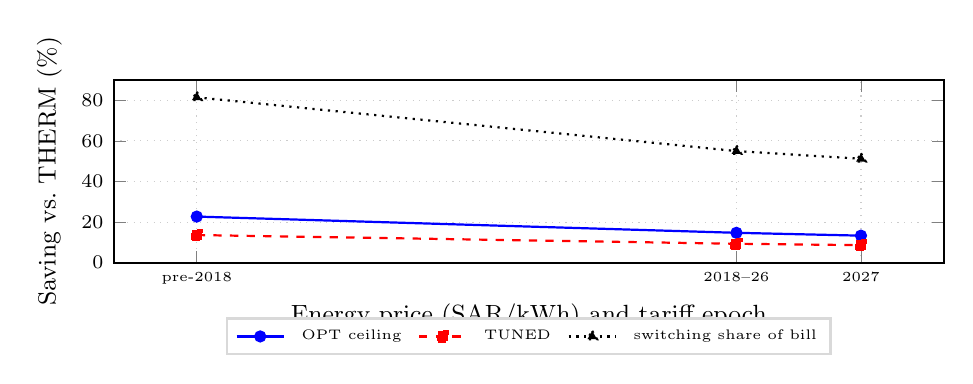
\begin{tikzpicture}
\begin{axis}[
  width=\linewidth, height=3.9cm,
  grid=major, grid style={dotted,gray!40},
  tick label style={font=\scriptsize},
  label style={font=\small},
  legend style={at={(0.5,-0.30)},anchor=north,legend columns=3,
                font=\tiny,draw=gray!30,column sep=4pt},
  thick,
  xtick={0.05,0.18,0.21}, xticklabels={pre-2018,2018--26,2027},
  xticklabel style={font=\tiny},
  xmin=0.03, xmax=0.23,
  xlabel={Energy price (\SAR/\kWh) and tariff epoch},
  ylabel={Saving vs.\ THERM (\%)},
  ymin=0, ymax=90,
]
\addplot[blue,thick,mark=*,mark size=1.8pt]
  coordinates{(0.05,22.7)(0.18,14.7)(0.21,13.3)};
\addlegendentry{OPT ceiling}
\addplot[red,thick,dashed,mark=square*,mark size=1.8pt]
  coordinates{(0.05,13.6)(0.18,9.3)(0.21,8.6)};
\addlegendentry{TUNED}
\addplot[black,dotted,thick,mark=triangle*,mark size=2pt]
  coordinates{(0.05,81.5)(0.18,55.0)(0.21,51.2)};
\addlegendentry{switching share of bill}
\end{axis}
\end{tikzpicture}
\caption{The reported saving is a function of the tariff, not only of the
controller. As the energy price rises, the switching component's share of the
baseline's bill falls from $81.5\%$ to $51.2\%$, and the percentage saved by
the tuned rule and by a clairvoyant schedule falls with it. What the $2018$
reform changed is the denominator, not the quantity recovered: the
\emph{absolute} saving is almost invariant across the three prices
(Section~\ref{subsec:disc_tariff}), so what a scheduler recovers here is a fixed
amount of deferred compressor wear and the percentage moves only because the
bill it is divided into grows. A saving quoted against a pre-reform price is
therefore not comparable with one quoted against the price in force, which
bears directly on the comparison with earlier studies in
Table~\ref{tab:sota}. Held-out
protocol, Riyadh, $\csw=0.15\,\SAR$; identical to
Table~\ref{tab:sensitivity}(a).}
\label{fig:tariff}
\end{figure}


In Riyadh the comparator's deadband moves the saving by $35$ points across
its admissible range, the controller class by $13$ (guard $5.7$, TUNED $12.5$,
$24\,$h controller $18.3\%$), the charge per on-command by $7$ across the
derived range and the tariff by $7$ across the three epochs (Table~\ref{tab:sensitivity}).
Only the controller class is algorithmic. The actuation step moves the saving
further (Section~\ref{subsec:timestep}).

The band acts mainly through the baseline. Narrowing it gives an optimising
controller \emph{less} room, but THERM, which switches $0.5\,^\circ$C inside
each edge, cycles more often on a narrower band, so the saving rises; the band
was not swept under the protocol, so no figure is given. The narrower band is
appropriate for this stock (Section~\ref{subsec:sbc}), but any percentage
reported for binary scheduling must be read with the band it was measured on.

What does move electricity is the comfort target. Along THERM's own
equalisation curve on the held-out windows, inside the $24\,^\circ$C ceiling,
raising THERM's switching thresholds by $0.1\,$K (a $0.10$--$0.12\,$K warmer
occupied mean) lowers its electricity by about $0.9$, $1.4$ and $2.3\%$ in
Riyadh, Jeddah and Taif, at the price of a warmer room;
at matched comfort no switching policy changes it.

The tariff acts through the denominator. At matched mean temperature
scheduling cannot change the energy delivered, only the number of on-commands,
each worth $\csw$; TUNED avoids the same $22.8\%$ of the equalised baseline's
on-commands in Riyadh under all three epochs, and the percentage falls as the
bill grows ($18.6$, $12.5$ and $11.6\%$). A percentage quoted against one tariff
epoch is not comparable with one quoted against another. With a constant
marginal price (Remark~\ref{rem:current_tariff}) and no time-of-use element,
the store the dwelling holds ($0.89\,\kWh$ electrical equivalent across the
band) has nothing to be sold into; a time-varying price would change that.

Where, then, could a controller save money rather than on-commands? The
receding-horizon controller and the clairvoyant bound already choose the whole
temperature path inside the band at every step, coupled rooms included, and
they do not pre-cool: with a single-speed unit, a constant COP and a flat price,
cooling earlier only adds the energy the store leaks. Electricity at matched
comfort becomes policy-dependent only when the cost of \emph{delivered} cooling
varies over the day, through a COP that rises at night (the $15$--$20\%$ of
Section~\ref{subsec:rules}), a time-of-use price, or a multi-speed or
inverter unit whose part-load efficiency differs from full load. None of these
is modelled here, so the conclusions hold for single-speed on/off units under a
flat tariff; a controller that chooses speed and timing jointly across coupled
rooms under those conditions, with setback in every room, is the natural next
study.

The same distinction governs what the work offers the national targets. At
matched comfort the controllers studied here change on-commands, not
electricity, so their contribution to emission cuts is indirect, through fewer
compressor cycles. Electricity, and with it emissions at a given generation mix,
moves with the comfort target and with the outdoor air: lowering Riyadh's
outdoor temperature by $1.5$ and $2\,$K, the Green Riyadh aim, cuts THERM's
cooling electricity on the held-out weeks by $10.5$ and $13.7\%$, while TUNED's
raw saving stays at $12.8$--$13.6\%$, so a cooler city and better switching add
rather than compete. The shift is applied to an airport weather year with the
plant and thresholds unchanged; it is a first-order sensitivity, not a model of
the urban heat island.

\subsection{Limitations}
\label{subsec:limits}
\label{subsec:disc_limits}

Supplementary Table~S6 gives the direction in which each idealisation biases
the reported percentage.
\begin{itemize}[leftmargin=*,itemsep=1pt,topsep=2pt]
\item \emph{The saving is specific to six modelling choices.} The comparator's
deadband, the actuation interval, the charge per on-command, the tariff, the
assumed thermal capacity and the thermostat's setpoint resolution each move
the headline by more than the resolution of the comparisons
(Tables~\ref{tab:sensitivity} and~\ref{tab:timestep}; Supplementary
Tables~S1 and~S2), and the comfort band, which was not swept, acts on it
through the baseline (Section~\ref{subsec:disc_band}); any figure quoted
from this paper should be quoted with all of them. The deadband sweep is capped
at $1.25\,^\circ$C by sampling the comparator at $15\,$min, and the
comparator's $1\,^\circ$C deadband is assumed, not measured.
\item \emph{Tied to the $15$-min step.} The savings depend on the actuation
step and the resolution at which the unit can be switched: TUNED saves about
$25\%$ at $5\,$min and $-1.2$ to $-1.5\%$ at $30\,$min
(Section~\ref{subsec:timestep}).
The comparator is a $1\,^\circ$C hysteresis evaluated at the actuation step; a
thermostat that senses continuously is not represented, and the saving
against it is not established. The headline numbers are not transferable to
other control steps.
\item \emph{On-commands, not compressor starts.} The model issues supervisory
on-commands to a lumped node; whether each is a compressor start depends on
the unit's own thermostat, and the model's on-command rate is an artefact of that interface, not a field
prediction.
\item \emph{Single-node thermal network and assumed capacity.} Air and fabric
share one capacitance. \citet{Bacher2011}, whose
identification framework is followed, rejected the single-state model for the
building they measured, because its residuals were not white, and selected a
four-state grey-box model; a plant with a separate air node would cycle faster
than this one. The capacity is assumed, and both results depend strongly on it
(Section~\ref{subsec:ladder}). ISO~13786's value is a $24\,$h quantity; the
capacity acting at the period of THERM's cycle is probably lower, towards
$2{,}400\,\text{kJ/K}$, where TUNED has no resolved saving, so the reference
results lean towards the end favourable to TUNED.
\item \emph{Thermostat resolution.} TUNED's switch points are fitted on a
$0.01\,^\circ$C grid; restricted to the $0.1\,^\circ$C steps of a real
thermostat it saves $5.7$, $7.4$ and $8.4\%$ instead of $12.5$, $13.6$ and
$12.4\%$, so the commissioning gain depends on hardware that can resolve the
thresholds. The guard and RBRL ceilings are fitted on the same fine grid.
Comfort matching to hundredths of a kelvin and every switch point assume
noise-free sensing for every arm, whereas typical thermistors err by a few
tenths of a kelvin.
\item \emph{Perfect model and forecast.} The receding-horizon controller plans
on the plant's own model with the exact state and, in its perfect mode, the
true in-horizon weather; the persistence mode removes the second idealisation
but not the first, and model mismatch is untested. Its terminal rollout uses
persistence weather and the TUNED rule, so no closed-loop dominance over TUNED
is guaranteed. The PPO agent's one-hour outdoor value is also exact.
\item \emph{Window-end terminal effect.} The terminal store is priced at
re-cooling energy without an on-command charge, so an oracle that knows the
window end can save up to one on-command per window, and in an earlier run
under that terminal CLV ended its windows markedly warmer than THERM. The
oracles therefore use $V_N$, which charges one on-command per kelvin left
above the start temperature; that rate is a convention.
\item \emph{Plant data.} The $2\,$kW capacity and the COP of $2.985$ are
assumed, not taken from a rated unit. The COP lies below the SASO~2663:2018
minimum for split units at the T1 rating condition (about $3.46$) though above
its T3 minimum (about $2.43$) \citep{SASO2663}. A higher COP lowers the energy term and so
raises the on-command share of cost and the percentage saving. Capacity and
COP are constant, whereas a split unit loses capacity and efficiency at high
outdoor temperatures; lower capacity acts in the hottest hours like a higher
$\Cth$ in the actuation ratio. An outdoor-dependent COP
(capacity held constant) is implemented in the repository but not reported;
the effect of either derating on the comparison is not established.
\item \emph{No per-start energy and no internal gains.} An on-command costs
money but no energy, so it cannot register as an energy saving; a transient
start-up loss of $10$--$25\,$Wh would turn TUNED's energy difference into a
saving of $0.33$--$0.80\%$ in Riyadh, $0.37$--$0.90\%$ in Jeddah and
$0.34$--$0.83\%$ in Taif. Occupancy, lighting and appliance gains, of order
$150$--$300\,$W in an occupied room and so comparable with the modelled
envelope load, are omitted, as is solar gain on opaque walls (an
intermediate-floor room is modelled). They shorten free-float and lengthen
on-phases, which is the mechanism the capacity and step sweeps act through;
their effect on the headline savings is not established, and they flatter
any setback's recovery.
\item \emph{Comfort offsets.} Rule~C does not cancel a difference in comfort
between arms: along the guard family a $0.01\,$K warmer mean is worth about
$1.3$ points, so the $3$-point resolution rule corresponds to about $0.02\,$K,
below Rule~A's $0.03\,$K tolerance. Arms whose $\Delta\tilde T$ differs by
more than about $0.02\,$K, including those fitted at the $0.10\,$K fallback,
are compared with that caveat. The admission rule itself matters: refitting
under a per-window $0.03\,$K criterion moves TUNED by up to $8.4$ points and
reverses F4 in Taif (Supplementary Table~S2); the receding-horizon controllers
were not refitted under it, so the robustness of F2 and F3 to the admission
rule is untested. Where the $\lambda$ device cannot reach the matched comfort level, the
receding-horizon controller is matched by backing off its occupied ceiling,
and a negative saving there is a finding about the device, not a failure of
the protocol.
\item \emph{Latent load.} The model is sensible-only. The latent axis was not
tested at adequate fidelity, so for Jeddah, whose infiltration load is
majority latent, this paper reports cost at matched dry-bulb comfort only, and
not compliance with the ASHRAE~55 humidity criterion.
\item \emph{Scope of the learner.} PPO is tested only inside the rule layer and,
in E2 (Riyadh, three seeds), with one comfort-aware reward; learners acting
outside R1--R2 are untested; longer training is not run, but on the tuning
weeks the trained policies already sit within $0.9\%$ of the hold policy's
training cost, except one Taif seed ($1.4\%$), so it has little to gain. R1 and R2 impose no minimum
dwell, so the complete-cycle structure is not enforced; a minimum-dwell rule
set is required work.
\item \emph{One year, one zone type, simulation only.} The held-out weeks are
interleaved within one TMYx year; the headline is a single zone with one
exposed face; the multi-zone study is one city, independent units, the same
band in every room and no bound, and a shared capacity-limited plant is not
studied. Time-of-use or demand tariffs, minimum on- or off-times, a
temperature-dependent COP and multi-speed or inverter units are not evaluated,
and the conclusions do not extend to them; setback is evaluated in the single
zone only. No result is reported on
a community benchmark such as
BOPTEST \citep{Blum2021}, and co-simulation and hardware-in-the-loop tests are
required before any deployment.
\end{itemize}

\section{Conclusions}
\label{sec:conclusion}

Binary on/off cooling of Saudi residential split units was formulated as a
constrained optimisation with hard comfort constraints, a charge per
on-command and an energy cost, and every controller was selected and evaluated
under one protocol in Riyadh, Jeddah and Taif. Four findings emerge.

First, commissioning a two-parameter thermostat widens its deadband from the
assumed $1\,^\circ$C to $1.32$--$1.36\,^\circ$C and avoids $22$--$24\%$ of
on-commands in every held-out window, with electricity within $\pm0.5\%$;
priced at the derived $0.025$--$0.114\,\SAR$ per on-command this is worth
$2$--$19\,\SAR$ per room per cooling season. The gain is a statement about the
comparator as much as about tuning: against a $1.25\,^\circ$C deadband the
tuned thermostat saves $5.7\%$ in Riyadh instead of $12.5\%$, on a
$0.1\,^\circ$C setpoint grid it avoids $11$--$15\%$ of on-commands, and at its
own mean temperature it attains $62$--$65\%$ of the provable bound.

Second, the comparison depends strongly on the plant and the step. A $24\,$h
receding-horizon controller avoids $30$--$33\%$ of on-commands and adds
$4$--$6$ points of cost saving with a perfect in-horizon forecast; with a
persistence forecast, the only imperfect one tested, its margin is not
resolved. In Riyadh the tuned thermostat has no resolved saving at half the
reference capacity and saves $15.8\%$ at twice it, while the controller's
margin falls from $15.0$ to $0.4$ points; because the capacity acting over a
cycle is probably below the reference, the reference results lean towards the
end favourable to the tuned thermostat. At a $5$-min step it saves about
$25\%$ and at $30\,$min $-1.2$ to $-1.5\%$, so every figure here holds for a
$15$-min step only.

Third, PPO trained under hard rules reproduces the rules' hold policy in
Riyadh and Jeddah and falls below it in Taif, and a comfort-aware variant,
tested in Riyadh only, stays close to hold. Inside the guard's own fitted
thresholds neither lookahead nor learning adds a resolved margin; an exact
one-step shield in place of the rules' fixed margins reaches the tuned
thermostat's level on a latch, and inside the wider training rules a $24\,$h
controller gains about $6$ points over the guard in Riyadh and Jeddah. The
guarantee the guards give costs $6.8$ and $6.0$ points in Riyadh and Jeddah.

Fourth, at matched mean temperature every arm uses about the same electricity,
by an identity of the model, so the cost difference is a charge on avoided
on-commands, assumed to stand for wear; electricity follows the comfort
target, each $0.1\,$K warmer mean lowering THERM's by $0.9$--$2.3\%$, and with
the outdoor air, which $1.5$--$2\,$K cooler (the Green Riyadh aim) lowers it
by $10.5$--$13.7\%$ in Riyadh. The money
saved depends on the six modelling choices of Section~\ref{subsec:limits} and
on the comfort band, which was not swept. Occupancy setback raises the on-commands the tuned rule
avoids to $29$--$35\%$ and its cost saving to $17$--$20\%$. In Riyadh
dwellings of two and four rooms with independent units the tuned thermostat
saves $11.7$--$13.6\%$, against $12.5\%$ in the single zone, differences that
are not resolved, and a non-cooperative distributed receding-horizon controller
saves $15.7$--$16.1\%$, against $18.3\%$ in the single zone.

For this model instance three recommendations follow. (i)~Judge any learner or
planner against a thermostat whose deadband has been widened to what the band
and the actuation step admit, not against the factory deadband. In practice
such commissioning assumes a supervisory $15$-min control layer and thresholds
resolved to $0.01\,^\circ$C (on a $0.1\,^\circ$C grid the saving is
$5.7$--$8.4\%$), and no commissioning or hardware cost is set here against the
$2$--$19\,\SAR$ per season. (ii)~Check both sides of the actuation
condition~\eqref{eq:deadband_condition} and derive guard bands from the
per-interval excursion in each direction before trusting any reported saving.
(iii)~Report a saving with the band, the comparator's deadband, the charge per
on-command and the on-commands avoided, and do not present it as a bill
saving. Every figure is simulated, and field validation, with the installed
stock's deadband measured, is required before any deployment claim.

\backmatter

\bmhead{Funding}
This work was funded by the Deanship of Graduate Studies and Scientific Research, Taif University.

\bmhead{Author contributions}
\textbf{Hamzah Faraj:} Conceptualization, Methodology, Software,
Validation, Formal analysis, Investigation, Writing -- original draft, Writing
-- review \& editing, Visualization.

\bmhead{Data availability}
\emph{What is released.} The code is available at
\href{https://github.com/drhamzahfaraj/Hybrid-Rule-Constrained-PPO-for-Cost-Effective-Binary-HVAC-Scheduling-in-Saudi-Residential-Buildings}{\textcolor{blue}{the project repository on GitHub}},
archived on Zenodo at
\href{https://doi.org/10.5281/zenodo.24199676}{\textcolor{blue}{doi:10.5281/zenodo.24199676}}
(release v4.0-round4); the trained PPO models ($29\,$MB) are not in the archive,
are available from the author on request, and can be retrained from the code with
the stated seeds. It comprises
the thermal model, every controller and oracle, the protocol module that
applies Rules~A--C to every arm, the statistics, and the scripts that generate
every table from the results files, each of which records the code version
that produced it. A gate
of $188$ numerical invariants in nine classes (physical sanity, bound
consistency, accounting identities, parameter provenance, monotonicity,
decomposition closure, feasibility, the deadband actuation condition, and the
protocol checks on every results file) runs before any table is produced and exits non-zero on any failure;
the feasibility class retains some checks written for the band of an earlier
version of the model. The time-step and capacity comfort records of THERM in
Supplementary Table~S1 come from a separate THERM run on the first held-out
Riyadh week.
Code paths that the paper does not report (an outdoor-dependent COP, a
behaviour-cloning variant, a shared-plant multi-zone arbitration) are in the
repository and marked as unreported.

\emph{What is not available.} An exploratory pipeline that preceded this
study is archived in the repository (\texttt{archive/withdrawn-pipeline}) for
transparency only; it does not reproduce, and is not the source of, any number
or figure reported here.

\emph{Weather data.} All three records are TMYx files from
climate.onebuilding.org: Riyadh (WMO~404380, 2009--2022), Jeddah
(WMO~410240, 2009--2023) and Taif
(WMO~410360, 2009--2023) \citep{EPW2023}.
The source reserves its rights, so the EPW files are not redistributed;
\texttt{fetch\_weather.py} names each station file and verifies the downloaded
copy by SHA-256. The actual-year series of the inter-annual study are ERA5
reanalysis \citep{Hersbach2020} retrieved through the Open-Meteo archive API,
redistributed in the repository under CC~BY~4.0 with attribution (weather data
by Open-Meteo.com; contains modified Copernicus Climate Change Service
information).

\section*{Declarations}

\bmhead{Ethics approval and consent to participate}
This research does not involve human participants, animal subjects or sensitive data. Ethics approval and consent to participate are not applicable; consent for publication is not applicable.

\bmhead{Competing interests}
The author declares no competing interests.

\bmhead{Use of generative AI}
During the preparation of this work the author used Claude (Anthropic) for
language editing, code assistance and simulated peer review of the manuscript.
All analyses, results and conclusions were checked by the author, who reviewed
and edited the content as needed and takes full responsibility for the
publication.

\bibliography{references}


\end{document}